\documentclass[12pt, oneside, a4paper]{ctexart}
% Shared preamble and layout helpers for 实习日记本-模板.tex.
% This file is loaded immediately after \documentclass.
% chktex-file 1
% chktex-file 8

\usepackage{amsmath}
\usepackage{amssymb}
\usepackage{caption}
\usepackage{float}
\usepackage[{top=25.4mm, bottom=25.4mm, left=31.8mm, right=31.8mm}]{geometry}
\usepackage{graphicx}
\usepackage[breaklinks, colorlinks=false, hidelinks, bookmarks=false, pdfpagelabels=false]{hyperref}
\usepackage{newtxtext,newtxmath}
\usepackage{xcolor}
\usepackage{xeCJK}
\usepackage{tikz}

\pagestyle{empty}
\AtBeginDocument{
  \setCJKfamilyfont{zh}[Path=C:/Windows/Fonts/,Extension=.ttc,FontIndex=0,AutoFakeBold={2}]{simsun}
  \renewcommand{\CJKrmdefault}{zh}
  \renewcommand{\CJKfamilydefault}{zh}
  \newCJKfontfamily\diarySong[Path=C:/Windows/Fonts/,Extension=.ttc,FontIndex=0]{simsun}
  \newCJKfontfamily\diaryHei[Path=C:/Windows/Fonts/,Extension=.ttf,AutoFakeBold={2}]{simhei}
  \newCJKfontfamily\diaryFang[Path=C:/Windows/Fonts/,Extension=.ttf]{simfang}
  \newCJKfontfamily\diaryShu[Path=C:/Windows/Fonts/,Extension=.TTF]{FZSTK}
}
\newcommand{\sourcecite}[1]{\textsuperscript{\color{red}[#1]}}
\newcommand{\pagecanvas}[1]{
  \thispagestyle{empty}
  \begin{tikzpicture}[remember picture, overlay]
    #1
  \end{tikzpicture}
  \null{}
}
\newcommand{\basewest}[3]{
  \node[anchor=base west, inner sep=0pt] at
    ([xshift=#1, yshift=-#2]current page.north west) {#3};
}
\newcommand{\basecenter}[3]{
  \node[anchor=base, inner sep=0pt] at
    ([xshift=#1, yshift=-#2]current page.north west) {#3};
}
\newcommand{\northwest}[3]{
  \node[anchor=north west, inner sep=0pt] at
    ([xshift=#1, yshift=-#2]current page.north west) {#3};
}
\newcommand{\northcenter}[3]{
  \node[anchor=north, inner sep=0pt] at
    ([xshift=#1, yshift=-#2]current page.north west) {#3};
}
\newcommand{\ruleline}[3]{
  \draw[line width=0.45pt]
    ([xshift=#1, yshift=-#3]current page.north west) --
    ([xshift=#2, yshift=-#3]current page.north west);
}
\newcommand{\diaryFormFont}{\diaryFang\fontsize{18pt}{20pt}\selectfont}
\newcommand{\diaryBodyFont}{\diarySong\fontsize{14pt}{19pt}\selectfont}
\newcommand{\diaryJournalBodyFont}{\diarySong\fontsize{12pt}{15pt}\selectfont}
\newcommand{\diaryTableFont}{\diaryFang\fontsize{15pt}{17pt}\selectfont}
\newcommand{\diaryPageFont}{\diarySong\fontsize{16pt}{18pt}\selectfont}
\ctexset{
  section = {format = {\centering\diaryHei\bfseries\Large}},
  subsection = {format = {\diaryHei\bfseries\large}},
  subsubsection = {format = {\diaryHei\bfseries\normalsize}}
}
\newcommand{\fixedline}[1]{\noindent\makebox[0pt][l]{#1}\\}
\newcommand{\diaryDateRuleSegments}{%
  \draw[line width=0.45pt, line cap=butt]
    ([xshift=37.0mm, yshift=-54.35mm]current page.north west) --
    ([xshift=50.0mm, yshift=-54.35mm]current page.north west)
    ([xshift=55.8mm, yshift=-54.35mm]current page.north west) --
    ([xshift=65.1mm, yshift=-54.35mm]current page.north west)
    ([xshift=69.8mm, yshift=-54.35mm]current page.north west) --
    ([xshift=80.7mm, yshift=-54.35mm]current page.north west)
    ([xshift=95.0mm, yshift=-54.35mm]current page.north west) --
    ([xshift=108.0mm, yshift=-54.35mm]current page.north west)
    ([xshift=112.6mm, yshift=-54.35mm]current page.north west) --
    ([xshift=121.8mm, yshift=-54.35mm]current page.north west)
    ([xshift=126.6mm, yshift=-54.35mm]current page.north west) --
    ([xshift=137.5mm, yshift=-54.35mm]current page.north west);
}
\newcounter{journalpagecounter}
\setcounter{journalpagecounter}{0}
\newcommand{\journalpage}{
  \stepcounter{journalpagecounter}
  \pagecanvas{
    \basewest{147mm}{20mm}{\diaryPageFont 实\hspace{0.25em}习\hspace{0.25em}日\hspace{0.25em}记}
    \ruleline{31.5mm}{179mm}{26.5mm}
    \ruleline{32mm}{177mm}{273mm}
    \basewest{158mm}{280mm}{\diaryPageFont 第\hspace{0.4em}\thejournalpagecounter\hspace{0.4em}页}
  }
}

% chktex-file 1
% chktex-file 8

\begin{document}

\pagecanvas{
  \northwest{60mm}{45mm}{
\includegraphics[width=90mm]{assets/tongji-diary-logo.png}}
  \basecenter{105mm}{99mm}{\diaryShu\fontsize{56pt}{45pt}\selectfont 实习日记本}
  \basewest{42mm}{143mm}{\diaryFormFont 学\hspace{2.1em}院}
  \ruleline{78mm}{176mm}{147mm}
  \basecenter{127mm}{143mm}{\diaryFormFont 交通学院}
  \basewest{42mm}{158mm}{\diaryFormFont 专\hspace{2.1em}业}
  \ruleline{78mm}{176mm}{162mm}
  \basecenter{127mm}{158mm}{\diaryFormFont 车辆工程}
  \basewest{42mm}{173mm}{\diaryFormFont 学\hspace{2.1em}号}
  \ruleline{78mm}{176mm}{177mm}
  \basecenter{127mm}{173mm}{\diaryFormFont 2352670}
  \basewest{42mm}{188mm}{\diaryFormFont 学生姓名}
  \ruleline{78mm}{176mm}{192mm}
  \basecenter{127mm}{188mm}{\diaryFormFont 肖哲夫}
  \basewest{42mm}{203mm}{\diaryFormFont 接受单位}
  \ruleline{78mm}{176mm}{207mm}
  \basecenter{127mm}{203mm}{\diaryFormFont 中车南京浦镇车辆有限公司~等}
  \basewest{42mm}{218mm}{\diaryFormFont 地\hspace{2.1em}址}
  \ruleline{78mm}{176mm}{222mm}
  \basecenter{127mm}{218mm}{\diaryFormFont 南京市江北新区浦珠北路68号~等}
  \basewest{35mm}{233mm}{\diaryFormFont 指导教师姓名}
  \ruleline{78mm}{176mm}{237mm}
  \basecenter{127mm}{233mm}{\diaryFormFont 周凯、季元进、吉文、潘宇}
}

\newpage
\pagecanvas{}

\newpage
\pagecanvas{
  \basecenter{105mm}{42mm}{\diaryHei\fontsize{22pt}{22pt}\selectfont 大学生校外实习守则}
  \northcenter{105mm}{62mm}{
    \begin{minipage}{155mm}
      \diaryBodyFont
      \setlength{\parindent}{2em}
      \setlength{\parskip}{0pt}
      \par{}
      一、高校校外实习是高等教育同社会主义建设相结合的重要环节，是培养合格人才的重要保证，每个学生必须按照教学计划的要求，认真参加各种形式的校外实习活动，并自觉遵守本守则。\par{}
      二、严格遵守实习单位的有关规章制度。如有违反，学校应会同实习单位按有关规定严肃处理。\par{}
      三、自觉遵守劳动纪律、尊重实习带教人员，服从安排，严格执行安全操作规程。\par{}
      四、妥善保管实习需要而借阅的图纸、资料，严格遵守保密制度，防止泄密。\par{}
      五、认真写好实习日记，客观记录实习的内容、问题及心得。\par{}
      六、独立完成实习报告，系统总结、综合分析实习中的问题以及解决问题的方法和建议。\par{}
      七、实习结束时，必须如数归还所借用的劳防用品、工具、仪器、资料及生活用品，如有损坏或遗失应按规定赔偿。\par{}
      八、学生在实习期间造成伤残和死亡的，可按“大学生团体平安保险”有关规定给予赔偿。
    \end{minipage}
  }
}

\newpage
\pagecanvas{
  \draw[line width=0.45pt]
  ([xshift=29mm, yshift=-31mm]current page.north west)
  rectangle
  ([xshift=180mm, yshift=-249mm]current page.north west);
  \ruleline{29mm}{180mm}{44mm}
  \ruleline{29mm}{180mm}{57mm}
  \ruleline{29mm}{180mm}{70mm}
  \ruleline{29mm}{180mm}{197mm}
  \basecenter{105mm}{40mm}{\diaryTableFont 实习起迄日期}
  \basewest{32mm}{53mm}{\diaryTableFont 自}
  \basewest{50.2mm}{53mm}{\diaryTableFont 年}
  \basewest{65.1mm}{53mm}{\diaryTableFont 月}
  \basewest{80mm}{53mm}{\diaryTableFont 日起至}
  \basewest{107mm}{53mm}{\diaryTableFont 年}
  \basewest{121.9mm}{53mm}{\diaryTableFont 月}
  \basewest{136.8mm}{53mm}{\diaryTableFont 日止}
  \basecenter{43.5mm}{53mm}{\diaryTableFont 2026}
  \basecenter{60.45mm}{53mm}{\diaryTableFont 7}
  \basecenter{75.25mm}{53mm}{\diaryTableFont 6}
  \basecenter{101.45mm}{53mm}{\diaryTableFont 2026}
  \basecenter{117.2mm}{53mm}{\diaryTableFont 7}
  \basecenter{132.05mm}{53mm}{\diaryTableFont 16}
  \diaryDateRuleSegments
  \basecenter{105mm}{66mm}{\diaryTableFont 实\hspace{0.5em}习\hspace{0.5em}内\hspace{0.5em}容}
  \node[anchor=north, align=left, text width=134mm, inner sep=0pt] at
  ([xshift=105mm, yshift=-81mm]current page.north west) {
    \diaryTableFont
    \hspace*{2em}赴中车南京浦镇车辆有限公司、申通中车轨道交通车辆有限公司、上海地铁梅陇基地、上海阿尔斯通及上海动车段等单位开展现场认知实习，其中南京浦镇共5天，其他均为1天。\\
    \hspace*{2em}主要学习城轨车辆车体制造、转向架制造与检修、总装调试、动车组高级检修等工艺流程，了解车辆段运维组织及安全生产规范；同时认识轨道交通装备制造与检修企业的组织架构、业务范围、生产管理和企业文化等基本知识。
  };
  \basewest{31mm}{203mm}{\diaryTableFont 指导教师批阅意见：}
  \basewest{71mm}{246mm}{\diaryTableFont 指导教师签名}
  \basewest{151mm}{246mm}{\diaryTableFont 月\hspace{1.5em}日}
}

\newpage
\thispagestyle{empty}
\vspace*{-10mm}
\section*{目录}
\vspace{4mm}
\newcommand{\diarytocdots}{\nobreak\leaders\hbox{\(\mkern1.5mu\cdot\mkern1.5mu\)}\hfill\nobreak}
{\diaryJournalBodyFont
  \noindent\hyperlink{journal-day-0706}{\diaryHei 7月6日}\quad{}\hyperlink{journal-day-0706}{\diaryHei 星期一}\diarytocdots\hyperlink{journal-day-0706}{第1页}\par\vspace{3mm}
  \noindent\hyperlink{journal-day-0707}{\diaryHei 7月7日}\quad{}\hyperlink{journal-day-0707}{\diaryHei 星期二}\diarytocdots\hyperlink{journal-day-0707}{第5页}\par\vspace{3mm}
  \noindent\hyperlink{journal-day-0708}{\diaryHei 7月8日}\quad{}\hyperlink{journal-day-0708}{\diaryHei 星期三}\diarytocdots\hyperlink{journal-day-0708}{第9页}\par\vspace{3mm}
  \noindent\hyperlink{journal-day-0709}{\diaryHei 7月9日}\quad{}\hyperlink{journal-day-0709}{\diaryHei 星期四}\diarytocdots\hyperlink{journal-day-0709}{第12页}\par\vspace{3mm}
  \noindent\hyperlink{journal-day-0710}{\diaryHei 7月10日}\quad{}\hyperlink{journal-day-0710}{\diaryHei 星期五}\diarytocdots\hyperlink{journal-day-0710}{第14页}\par\vspace{3mm}
  \noindent\hyperlink{journal-day-0713}{\diaryHei 7月13日}\quad{}\hyperlink{journal-day-0713}{\diaryHei 星期一}\diarytocdots\hyperlink{journal-day-0713}{第15页}\par\vspace{3mm}
  \noindent\hyperlink{journal-day-0714}{\diaryHei 7月14日}\quad{}\hyperlink{journal-day-0714}{\diaryHei 星期二}\diarytocdots\hyperlink{journal-day-0714}{第18页}\par\vspace{3mm}
  \noindent\hyperlink{journal-day-0715}{\diaryHei 7月15日}\quad{}\hyperlink{journal-day-0715}{\diaryHei 星期三}\diarytocdots\hyperlink{journal-day-0715}{第21页}\par\vspace{3mm}
  \noindent\hyperlink{journal-day-0716}{\diaryHei 7月16日}\quad{}\hyperlink{journal-day-0716}{\diaryHei 星期四}\diarytocdots\hyperlink{journal-day-0716}{第23页}\par\vspace{3mm}
  \noindent\hyperlink{references}{\diaryHei 参考文献}\diarytocdots\hyperlink{references}{第26页}\par}

\newpage
\pagecanvas{}

\newpage
\journalpage
\vspace{-7.5mm}
\hypertarget{journal-day-0706}{}
\section*{7月6日\quad{}星期一}
\diaryJournalBodyFont\vspace{-3mm}\par{}
第一天我们来到浦镇厂报告厅听讲座，主要是介绍创新与研发体系、城轨车体制造工艺技术、转向架工艺设计流程与相关智能产线、城轨车辆总装工艺技术等；其中还穿插了安全教育，提醒大家在厂区内必须戴上安全帽、不要玩手机、不要在重物下停留、不能拍照等。\par{}
下文主要摘录讲座上记录的主要内容：\par{}
\vspace{-5mm}\subsection*{一、 创新与研发体系介绍}
\vspace{-2mm}\subsubsection*{1.1\quad{}基本概况}\vspace{-2mm}
{\bf{}组织架构：}技术中心下设7部门，分别为科技管理部、总体研发部、转向架研发部、结构研发部、电气研发部、设备研发部和试验中心等。\par{}
{\bf{}主要职能：}新造、加改、科研、支持。\par{}
{\bf{}部门职责：}科技管理部总管各研发部，总体研发部牵头整车项目设计等。\par{}
{\bf{}研发能力：}包括车体、转向架、TCMS等关键系统与产品的研发，网络软件的研发，静强度、碰撞、动应力、模态等的多学科仿真设计，系统工程设计，工业设计，基础研究及试验等能力，涵盖车辆设计生产制造全流程的研发任务。\par{}
\textcolor{gray}{{\bf{}tips: }这一部分中有相当一些知识是学过的，如仿真设计涉及轨道车辆设计课程中的有限元分析等知识，系统工程设计中包含了RAMS、LCC等可靠性核心概念，这些都是本学期必修或选修课的相关内容，学了之后就不再陌生了。}\par{}
\vspace{-5mm}\subsubsection*{1.2\quad{}技术创新成果}\vspace{-2mm}
{\bf{}产品平台：}动车组，如系列化动集（CR200J-A/B/C/D）、动分（CR300AF、CRH2G、CRH6）；客车，除常规客车外还有轨检车、隧检车、电检车、多功能后勤保障车等；城轨车辆，包括系列化地铁、市域铁路、中低运量列车，以及各类工程车产品。\par{}
{\bf{}专项技术：}包含车体轻量化、新材料、先进制造技术、服役寿命的研究，多种干线铁路客车、城轨车辆、城际市域车辆、胶轮车辆转向架的研发，一体化智慧列车运行系统TCSI、多系统/多网多屏融合技术、无线通信技术的专利等等。\par{}
{\bf{}研发体系：}通过数字化手段赋能研发设计业务，建立数据贯通、业务协同、管理规范的研发体系；对设计文件、表单、联系书等进行统型与规范化，制定文档模板等等。\par{}
{\bf{}专利获奖（略）}\par{}
\textcolor{gray}{{\bf{}tips: }同样有某些内容上课学过，如车体轻量化就可以通过采用中空铝型材等新材料，以及先进设计制造方法等方式进行。}\par{}

\newpage
\journalpage
\vspace{-7.5mm}\subsubsection*{1.3\quad{}研发未来展望}\vspace{-2mm}
新制式车辆平台建设（新产品）、新型轻量化材料应用（新材料）、新型设计方法应用（新方法）、新型电气架构（新架构）；设计能力提升与关键技术/系统应用，如模块化自主化设计、TCSI系统在中低运量列车上的运用、灵活编组技术的应用等；AI技术应用与智能运维赋能提升等。\par{}
\vspace{-5mm}\subsection*{二、 城轨车辆车体制造工艺技术概述}
\vspace{-2mm}\subsubsection*{2.1\quad{}车体结构简述}\vspace{-2mm}
{\bf{}车辆基本类型：}从车体材料上分，有铝合金铆接、铝合金焊接、不锈钢、碳钢等几种，从车辆形制上分，有低地板车辆、空轨车辆、跨座式单轨车辆、普通地铁列车/动车组等，{\bf{}车辆类型繁多，且每种车辆批量较小}。\par{}
{\bf{}材料：}车体主材大多采用铝合金，原因是其储量大、可回收、轻量化、能耗/磨耗小。铝合金中主要使用6000系（Al-Mg-Si）和7000系（Al-Zn）的热处理强化铝合金，如某型地铁列车大量采用6005A-T6牌号的铝合金做底架、侧墙、车顶、端墙、司机室等结构。此外还有焊接用材料，包括电焊条、焊丝、保护气等，其中保护气采用纯度高于$99.999\%$的氩气；焊接后还要对焊接前后的力学性能进行对比检验等。\par{}
{\bf{}车体结构：}$\mathrm{T_c}$车有驾驶室，无牵引电机；$\mathrm{M}$/$\mathrm{M_p}$车无驾驶室，有牵引电机；对于列车而言，车体就是轻量化骨架，转向架是行走的脚步，内装就是血肉，而铆接的密封性不如焊接，因此车体大都采用焊接的方式，部分列车或列车的某些部分仍然采用铆接；底架分为头部底架和中间车底架，对应头车和中间车，按有无司机室划分；底架使用铆钉连接至横梁，下挂电池、配重等；车顶也分为头车用和中间车用；侧墙有的分块安装，有的整块安装，各有优缺点；端墙上应预留贯通道的位置；司机室有防爬器等装置，部分还配备了逃生门等；车辆的编组连挂形式也多种多样。\par{}
\vspace{-5mm}\subsubsection*{2.2\quad{}车体制造工艺流程}\vspace{-2mm}
{\bf{}工艺流程：}底架、车顶、侧墙、端墙分别制造，成型后直接进行车体预组，再整车焊接、检查、交验等（图略）。具体而言主要分为底架组装、侧墙组装、端角柱组装、端墙组装、车顶组装、车顶定位焊、预组尺寸检测、车体焊接与检验等步骤。其中有一大特点就是焊接的数字化、自动化，不知此后几日是否可以观察到自动焊接的过程。\par{}
\vspace{-5mm}\subsubsection*{2.3\quad{}车体制造工艺方法}\vspace{-2mm}
{\bf{}基础工艺：}原则是保障安全、保证功能、保证美观，由于常用焊接、粘接、铆接、螺纹连接、电气压接等方式进行连接作业，因此对于粘接等环境要求较高\par{}

\newpage
\journalpage\par\noindent
的方式，需要进行严格环境把控，防止对列车的安全、功能、美观造成影响；螺栓连接也是，连接后应当进行防松和紧固处理，并对螺栓和接触部件做标记处理，可以显示其是否松动旋转。\par{}
{\bf{}焊接工艺：}铝合金除了常用的电弧焊等，还常用搅拌摩擦焊、激光焊、激光-电弧复合焊等新型焊接方式，各有优缺点和适用场景。搅拌摩擦焊就是通过搅拌工具的轴肩平面与板材的旋转摩擦，使得焊缝金属热塑化，又受压力的影响被挤压与锻造，从而形成接头。\par{}
{\bf{}激光清洗：}将高亮、高方向性的连续/脉冲激光照射至工件表面，振动、熔化、燃烧甚至气化表面的油污、锈蚀、涂层等，在不损坏材料本身的情况下使得污染物剥离，具有绿色环保、效率高、效果强、成本低等优点。\par{}
{\bf{}激光投影：}通过激光在短时间内快速投影线迹，避免人为因素影响，做到有方法可依。\par{}
\vspace{-5mm}\subsubsection*{2.4\quad{}数智制造工艺}\vspace{-2mm}
事后检→事前算，由于浦镇厂小批量生产居多且不断增加，因此需要进行数智化转型，减少换型时间；构建一车一档的数字履历，并把数据记录变为生产资本。\par{}
\vspace{-5mm}\subsection*{三、 转向架工艺设计流程介绍与焊接、组装智能产线介绍}
\vspace{-2mm}\subsubsection*{3.1\quad{}工艺流程}\vspace{-2mm}
{\bf{}构架工艺：}侧梁焊接工艺、横梁焊接工艺、构架组焊工艺、打磨工艺、尺寸检查工艺、构架探伤工艺、构架热处理工艺、构架加工工艺、构架涂装工艺等。\par{}
{\bf{}轮对工艺：}车轮轮毂孔加工工艺、车轴车削与磨削工艺、车轴油漆工艺、轮对压装工艺、轴承轴箱组装工艺等。\par{}
{\bf{}转向架总装工艺：}子部件预组工艺、挂件组装工艺、转向架落轮工艺、转向架交验工艺等。
\vspace{-5mm}\subsubsection*{3.2\quad{}工艺设计介绍}\vspace{-2mm}
包含投标支持、工艺策划、工艺性审查、工艺方案设计、工艺试验、工艺设计、模拟生产线、试制与总结、批量与售后等步骤。\par{}
\vspace{-5mm}\subsubsection*{3.3\quad{}智能产线介绍}\vspace{-2mm}
传统产线面临设备自动化率低、产品质量稳定性低、人工劳动强度高、过程数据孤立分散的问题，而智能产线可以解决这些问题。场内有构架焊接智能产线、转向架组装智能产线等。

\newpage
\journalpage
\vspace{-7.5mm}\subsection*{四、 城轨车辆总装生产工艺技术概述}
\vspace{-2mm}\subsubsection*{4.1\quad{}轨道车辆种类}\vspace{-2mm}
{\bf{}铁路干线客车：}25B/G/T、双层客车、内燃动车组、电动车组、高原客车、各类特种车辆等。\par{}
{\bf{}城轨/地铁列车：}A/B/C型地铁、低地板城轨、空轨等。\par{}
\vspace{-5mm}\subsubsection*{4.2\quad{}总装流程}\vspace{-2mm}
首先进行车体、转向架生产，并进行涂装（不再赘述），最后进行总装、精调、动调。\par{}
具体流程为：车体安装地板→玻璃粘接→地板布铺装→高站流水线（14台位）→预落轮→落车与连接→称重试验→电调门→限界试验→门边立罩与侧顶板调节→外部标识安装→静调→动调→内部标识粘接。\par{}
\vspace{-5mm}\subsubsection*{4.3\quad{}基础工艺方法}\vspace{-2mm}
包含螺栓、铆接、粘接、电气连接等，不再赘述。\par{}
\vspace{-5mm}\subsubsection*{4.4\quad{}数智制造工艺}\vspace{-2mm}
这一部分的数智生产线主要包含车体焊接产线、自动化涂装产线、玻璃粘接产线、数字化总装产线、数字化调试产线等；员工还可以使用智能扭力扳手进行作业，以记录数据、进行监测等，还有智能工具箱可以对工具进行管理；设计方面可以使用DFM进行三维工艺设计等。\par{}
未来总装智能产线的发展方向主要有机器人与自动化、AI、大数据分析、VR/AR协同、柔性与个性协同、绿色生产等（略）。\par{}
\subsection*{小结}
总的来说，今天主要了解了浦镇厂的基本情况，同时也对列车部件的生产制造工序有了一定的了解，为日后的参观实习打下了基础。另外值得一提的是厂里饭堂口味还不错，才16块一顿，就有两大荤一小荤一素+米饭+汤+饮料，量大管饱，味道也挺好。\par{}

\newpage
\journalpage
\vspace{-7.5mm}
\hypertarget{journal-day-0707}{}
\section*{7月7日\quad{}星期二}
\diaryJournalBodyFont\vspace{-3mm}\par{}
今天主要参观了企业文化展厅和转向架分厂。\par{}
\vspace{-5mm}\subsection*{一、 参观企业文化展厅}\vspace{-2mm}
上午在企业文化展厅主要了解了厂区的历史、布局和产品，下面是一些图片：\par{}
\begin{figure}[H]
  \centering
  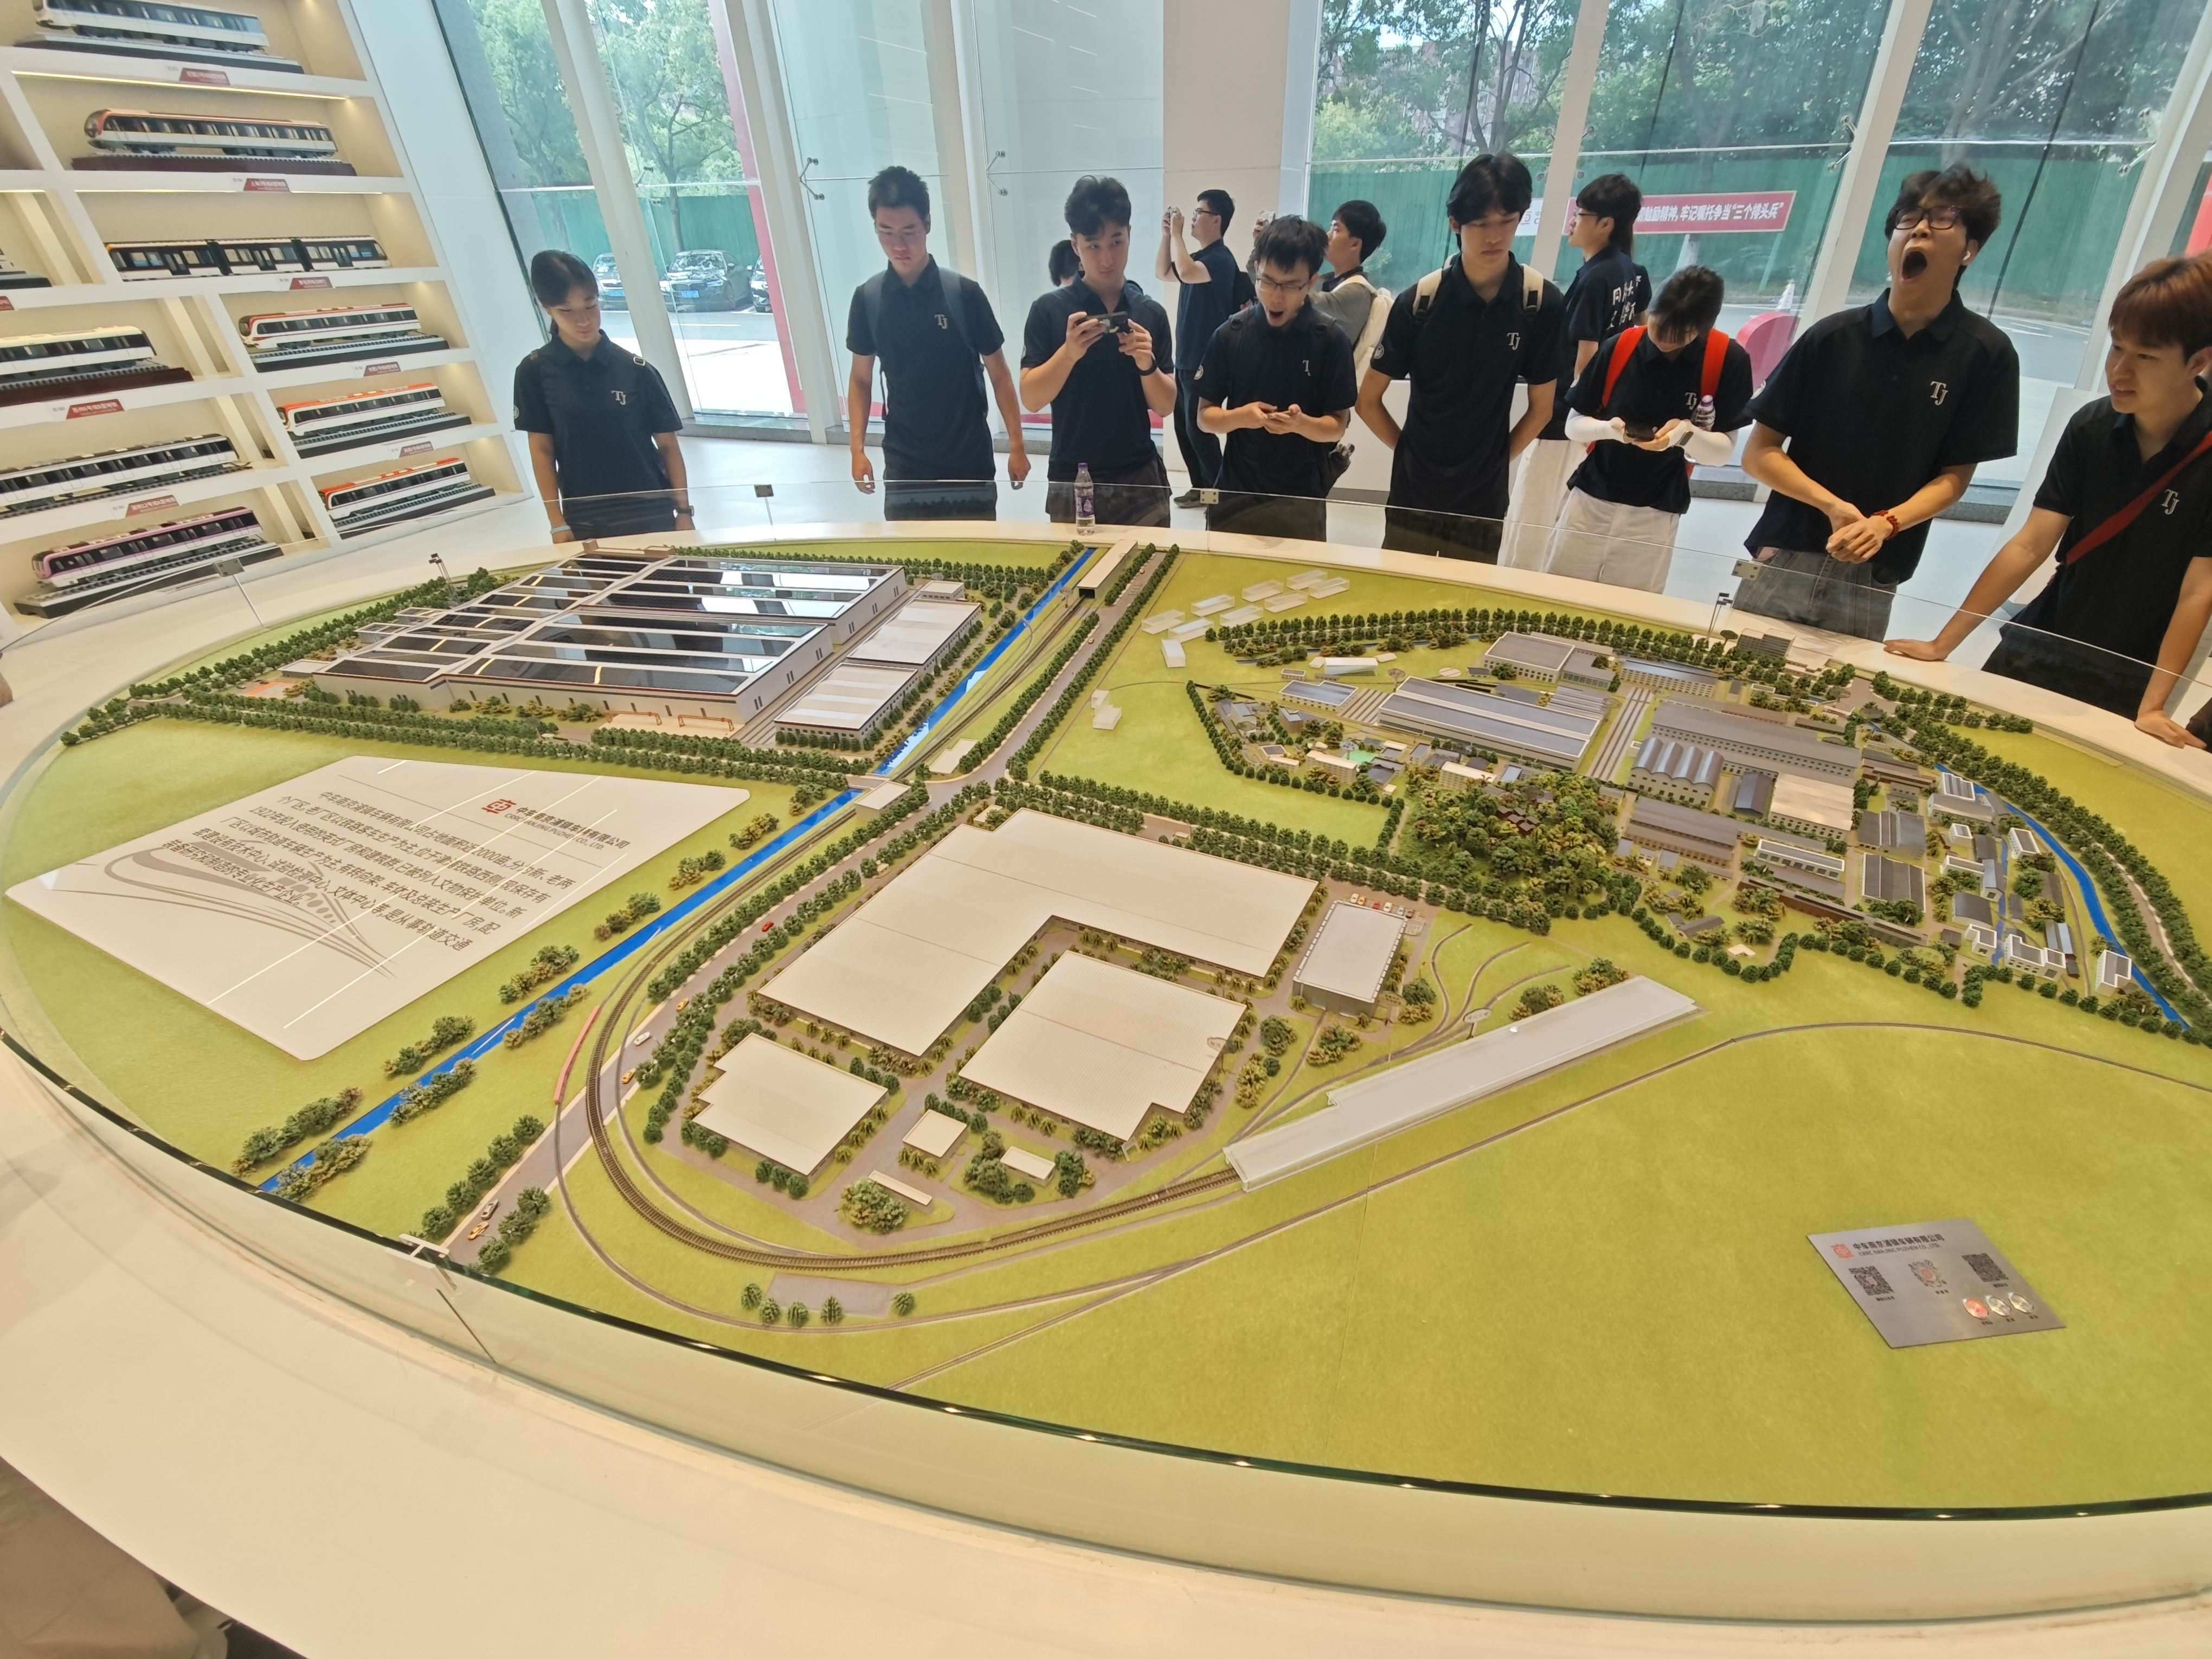
\includegraphics[width=0.8\textwidth]{assets/20260709_122254.jpg}
  \vspace{-2.5mm}
  \caption*{\small{}图1\quad{}厂区模型}
  \vspace{2.5mm}
  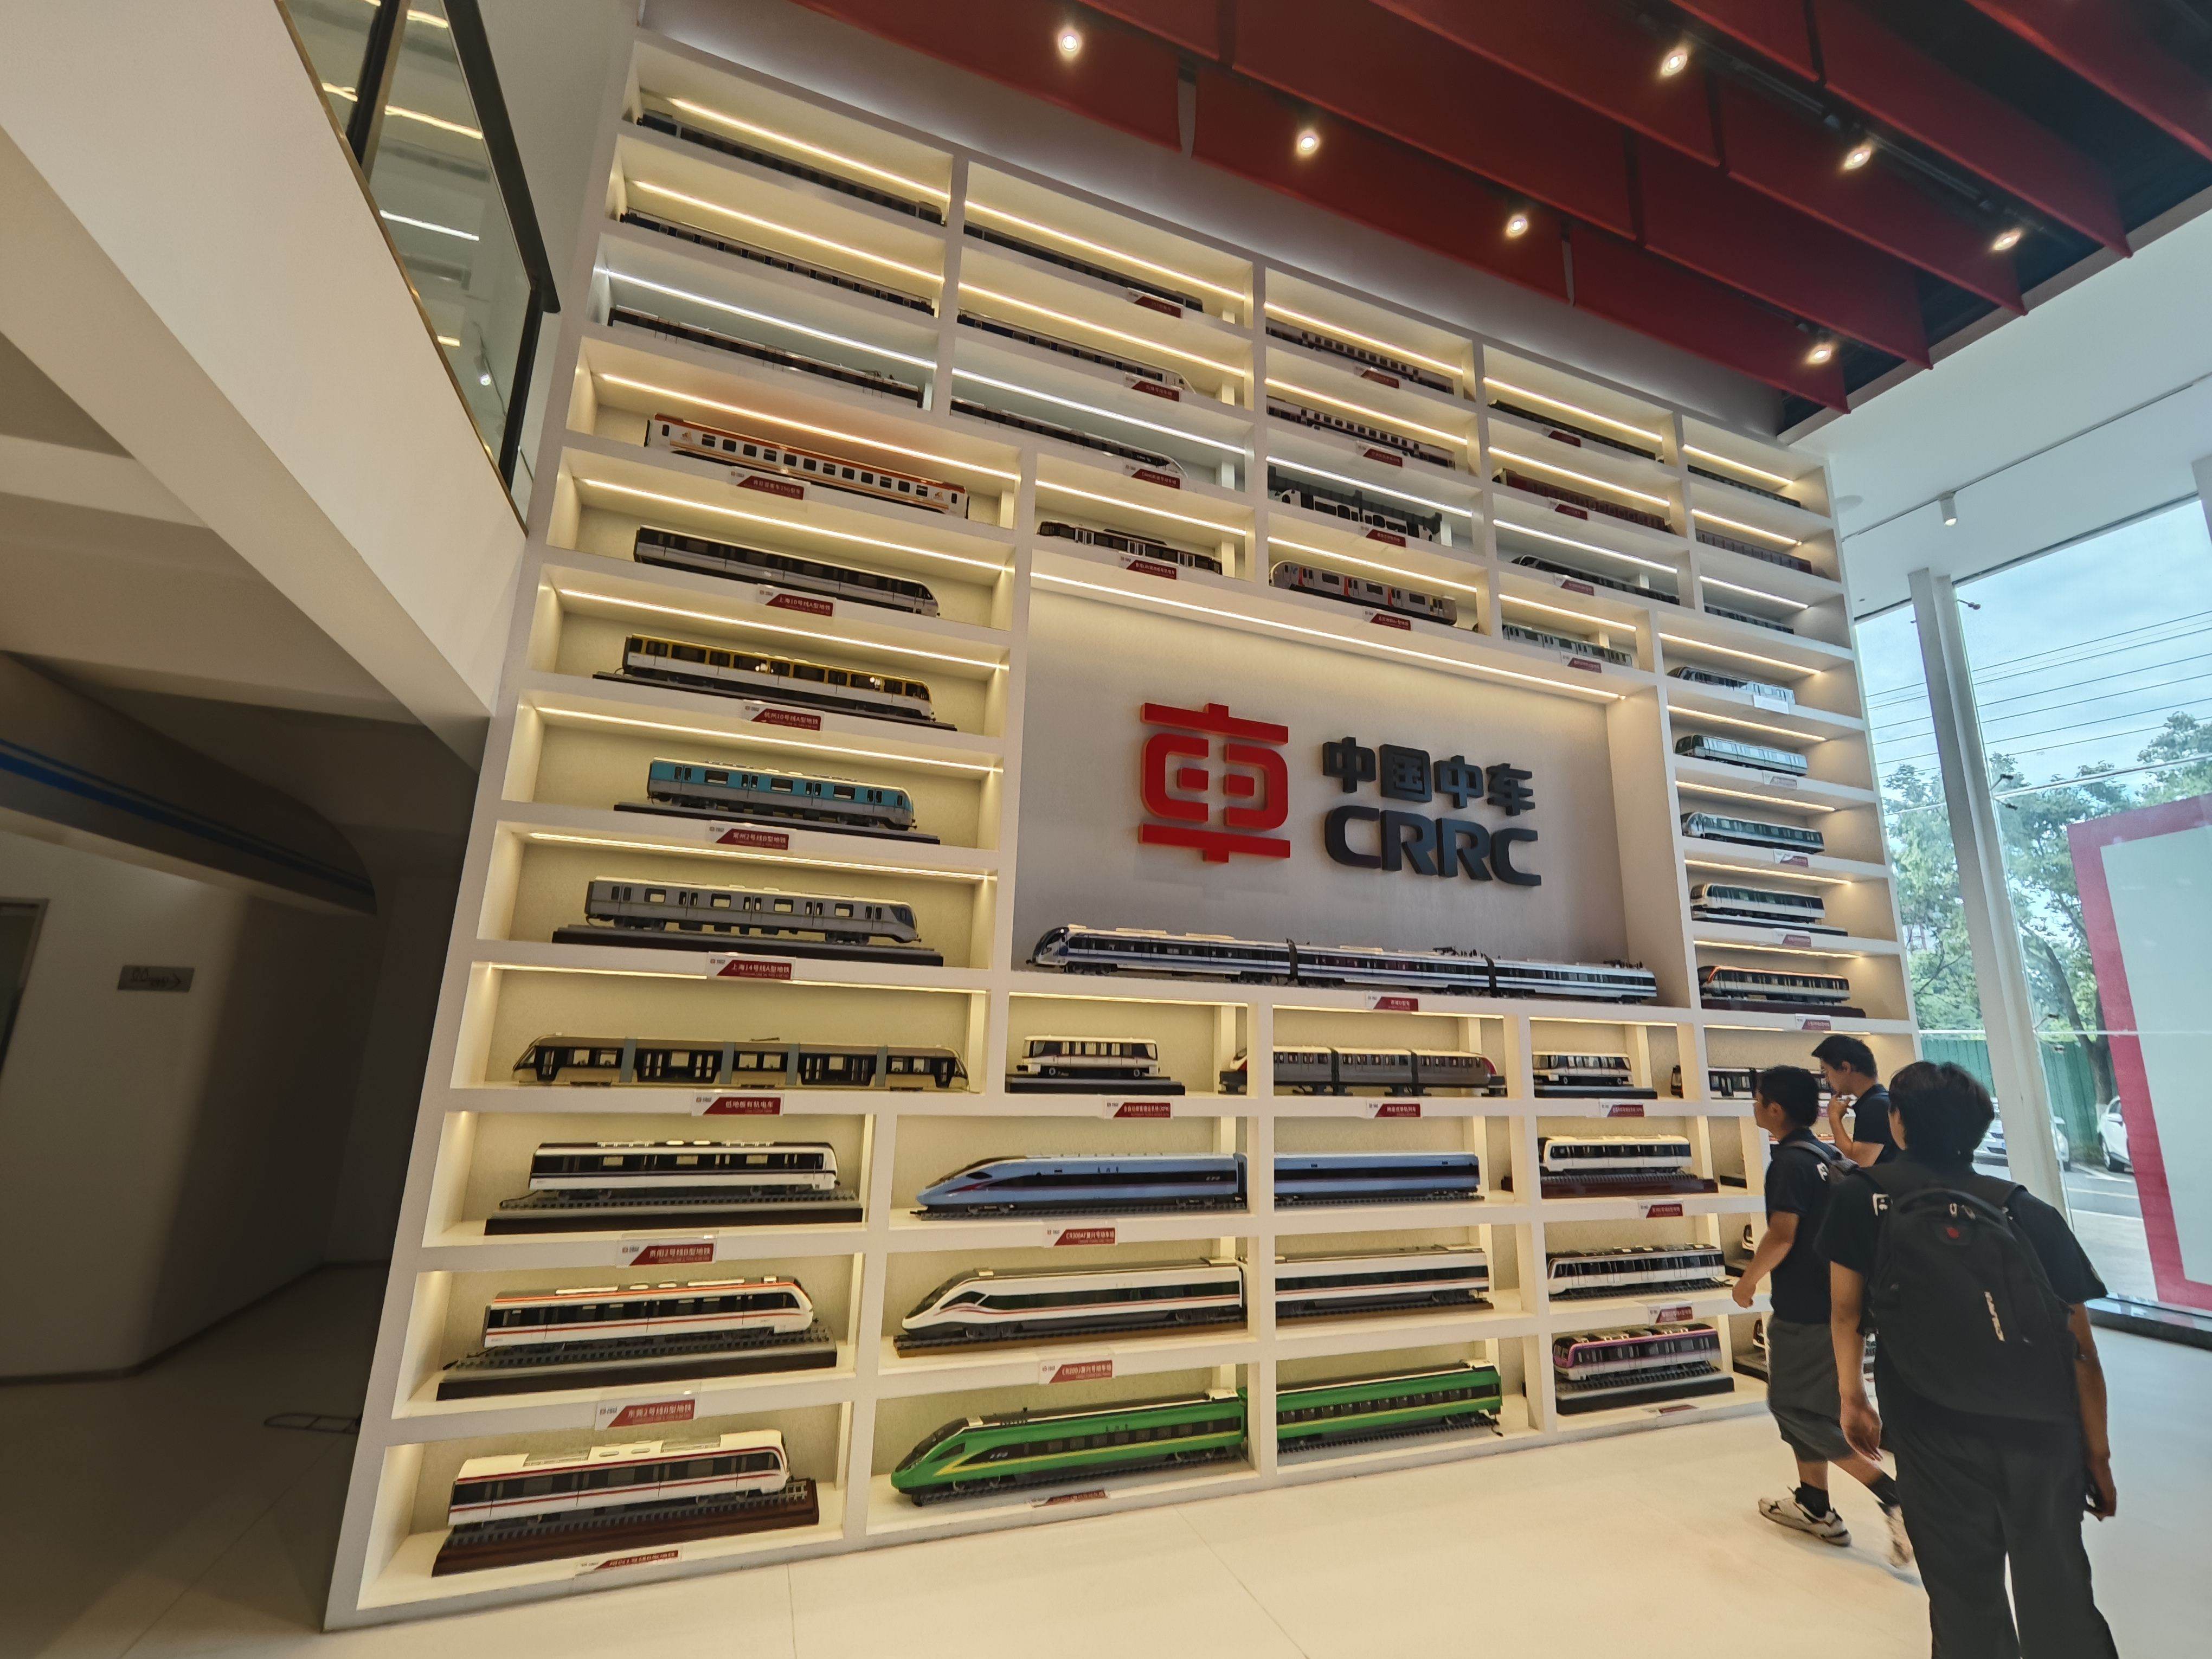
\includegraphics[width=0.8\textwidth]{assets/20260709_122305.jpg}
  \vspace{-2.5mm}
  \caption*{\small{}图2\quad{}浦镇产各式车辆模型}
\end{figure}

\newpage
\journalpage\par\noindent
\begin{figure}[H]
  \centering
  \vspace{20mm}
  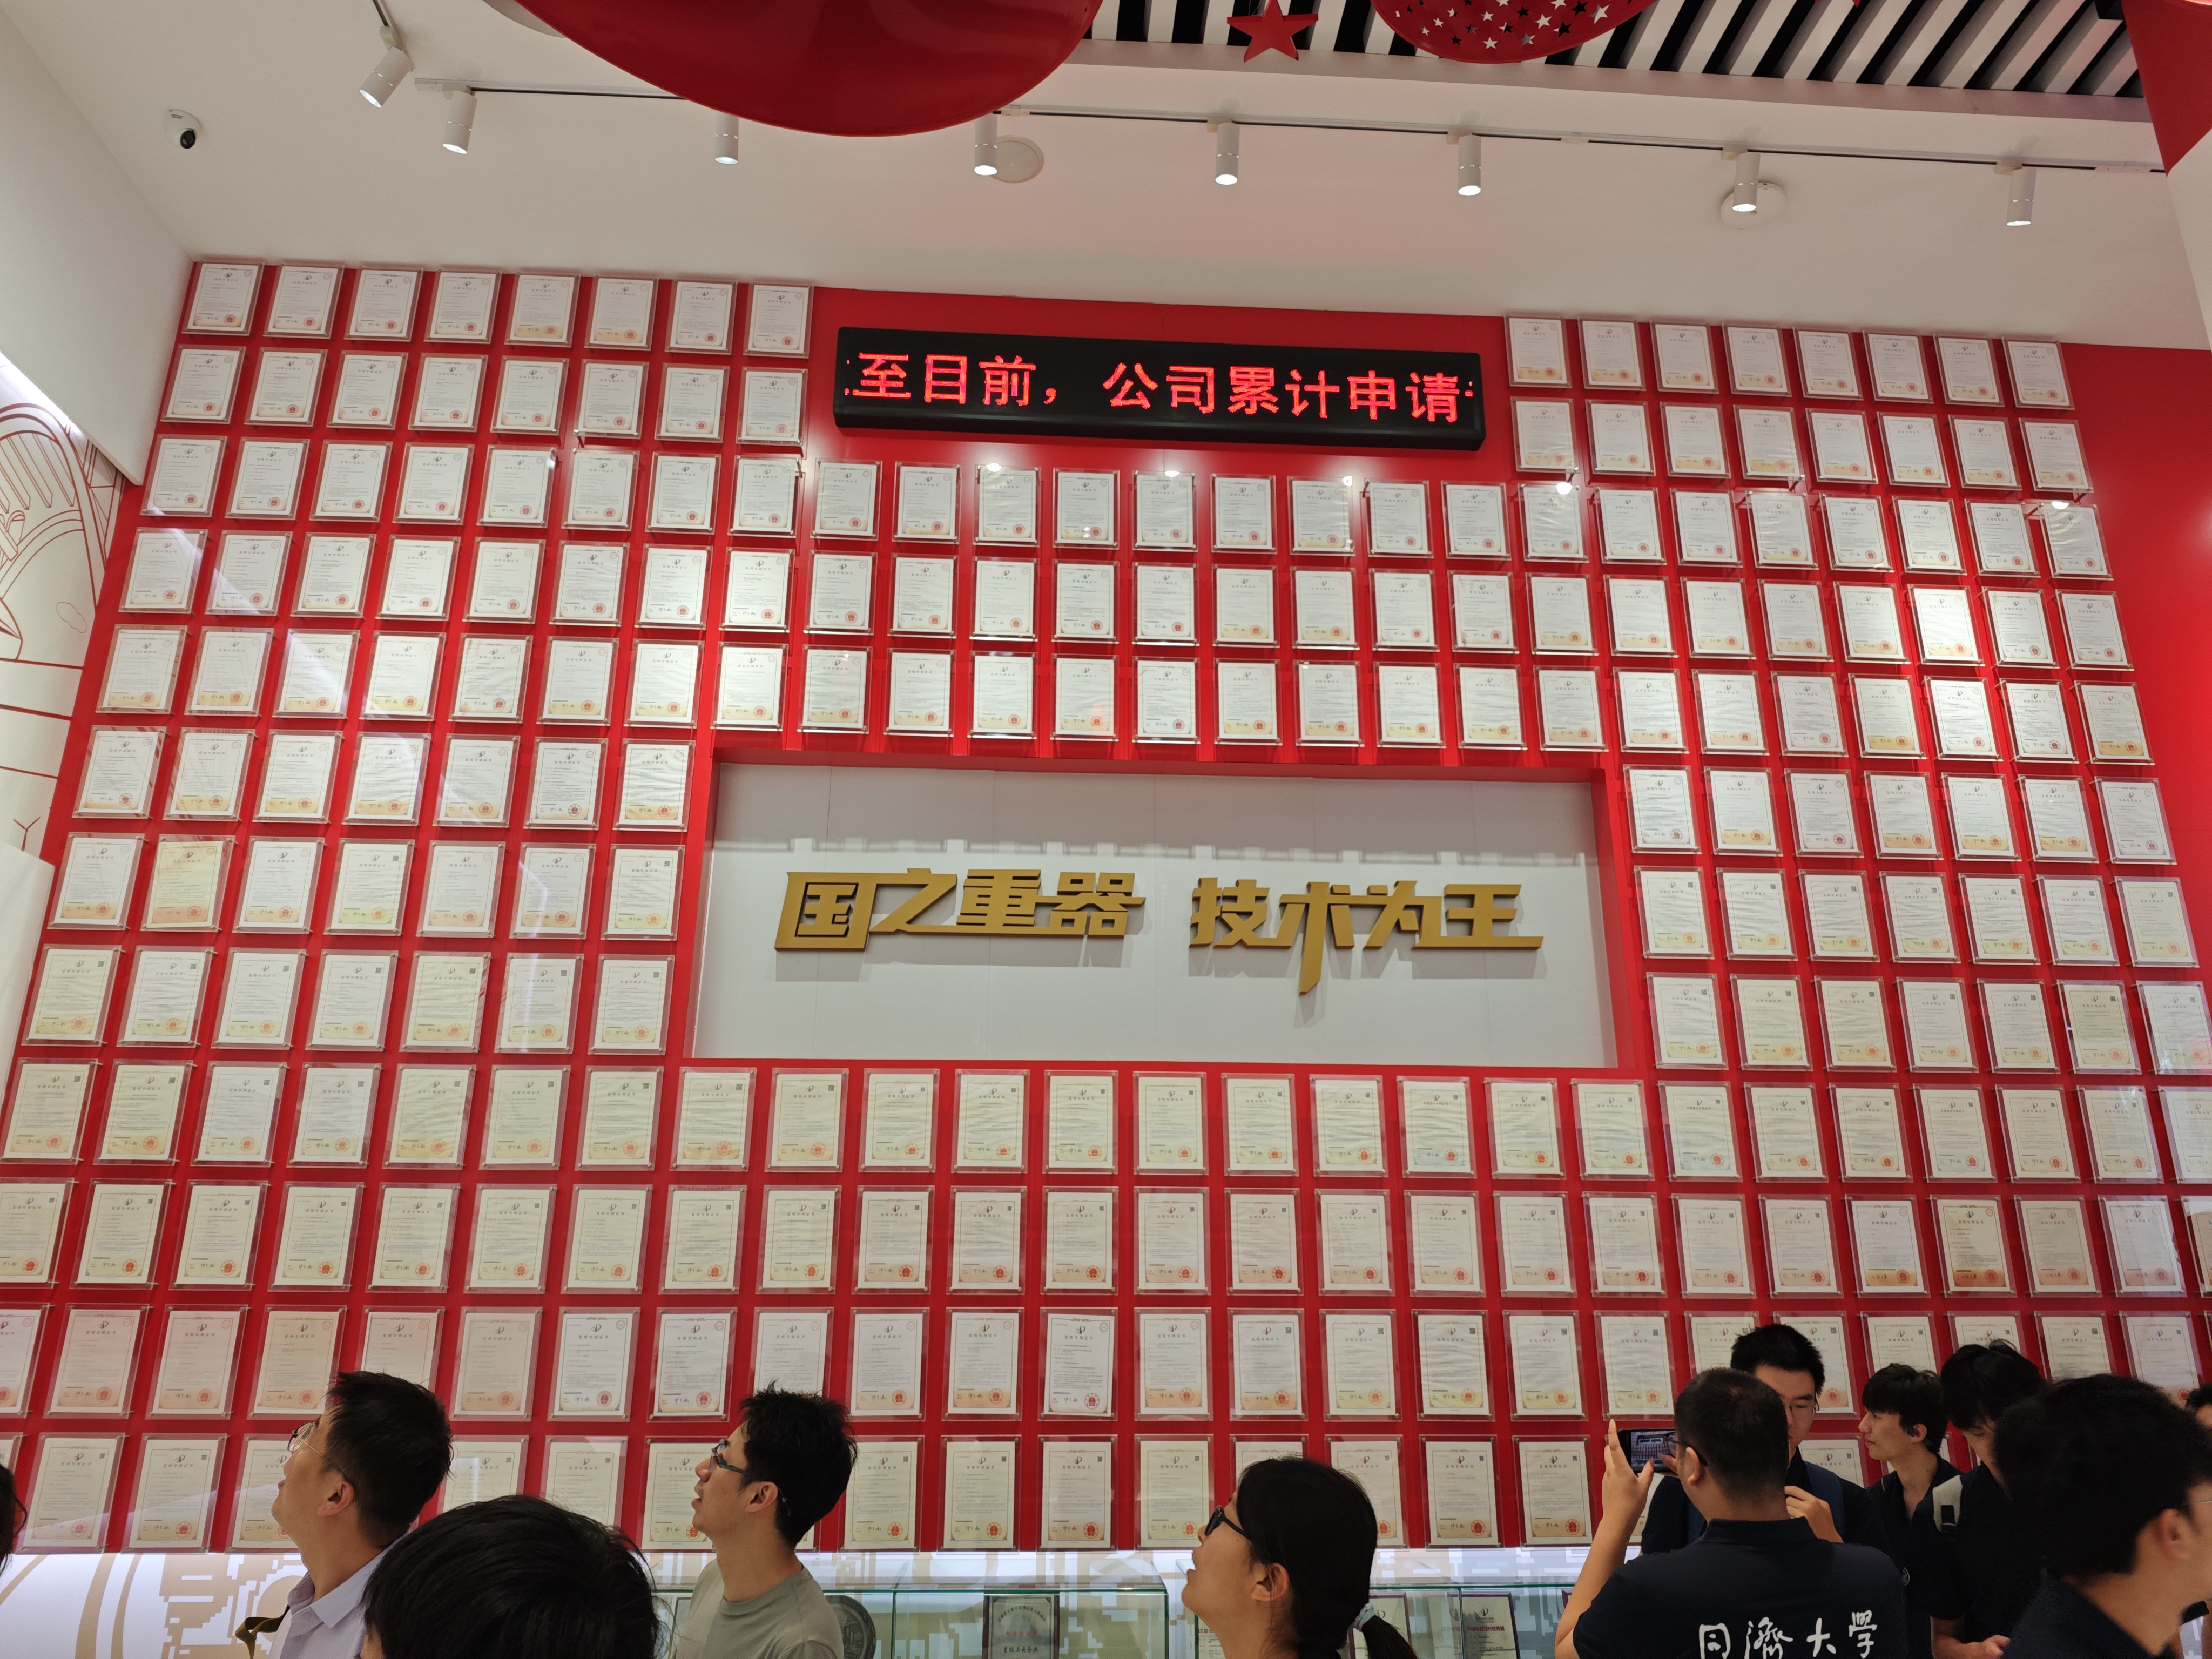
\includegraphics[width=0.8\textwidth]{assets/20260709_122307.jpg}
  \vspace{-2.5mm}
  \caption*{\small{}图3\quad{}浦镇厂获得的各类专利证书}
  \vspace{2.5mm}
  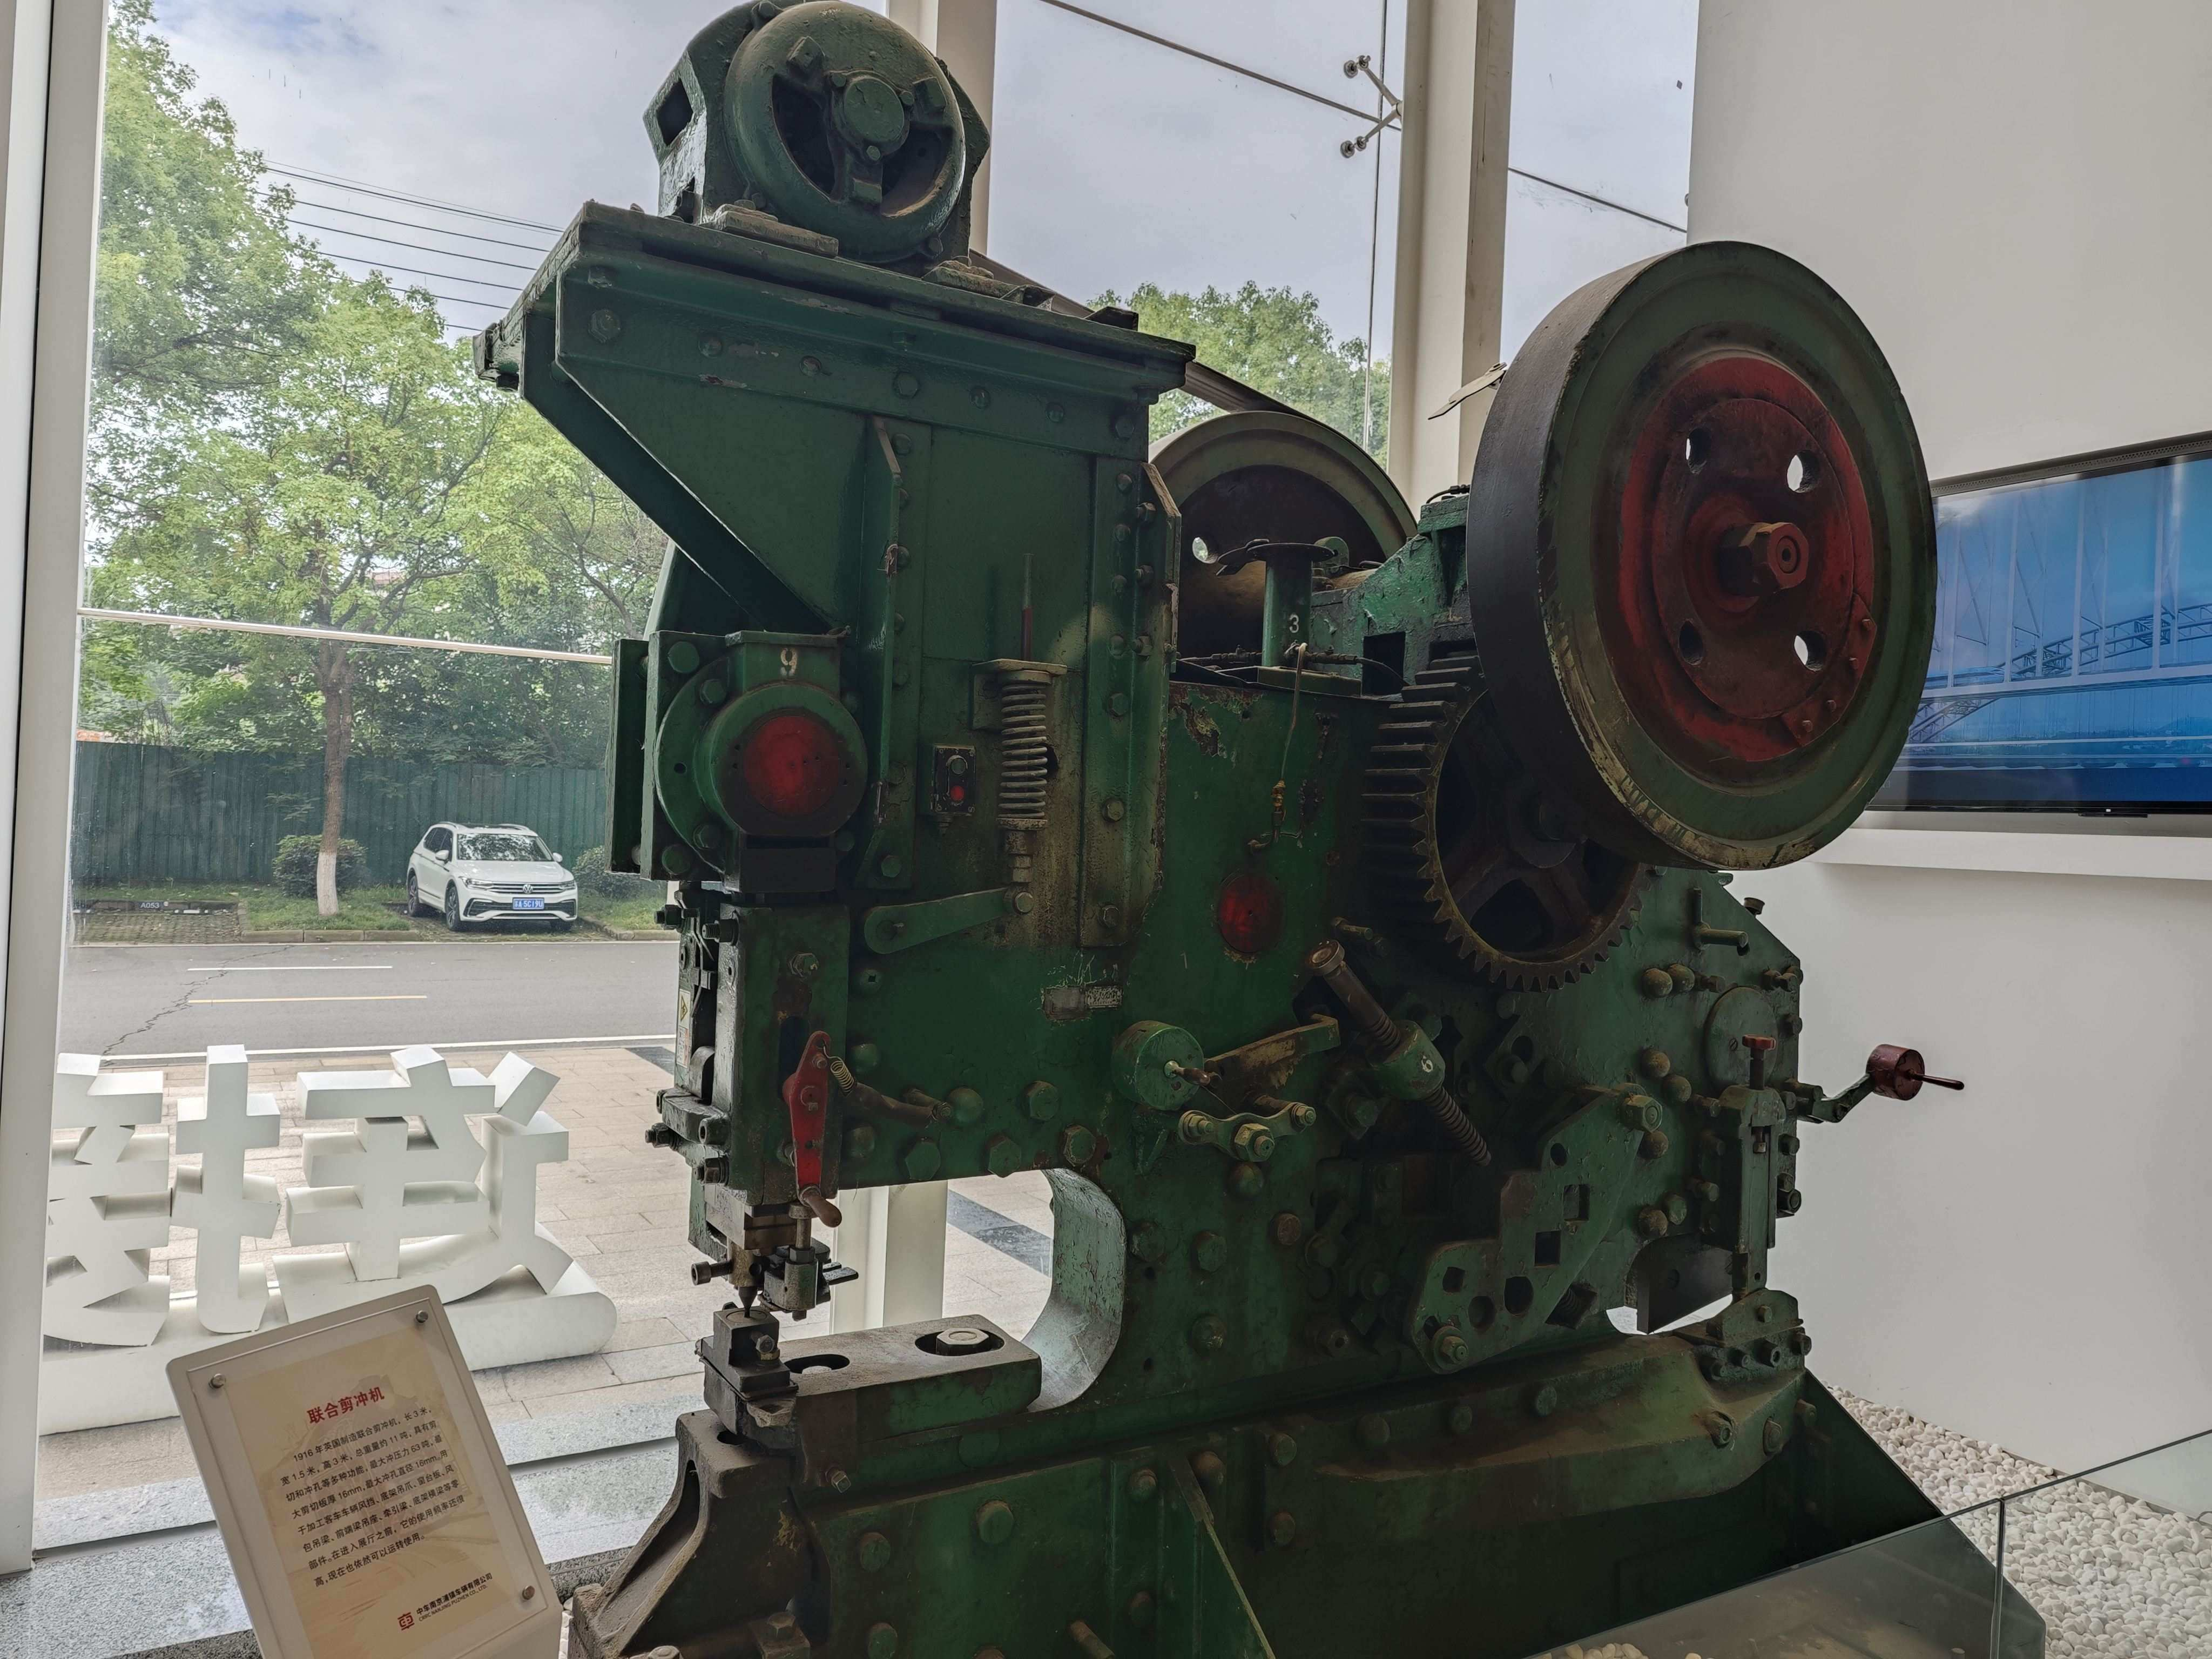
\includegraphics[width=0.8\textwidth]{assets/20260709_122308.jpg}
  \vspace{-2.5mm}
  \caption*{\small{}图4\quad{}浦镇厂老式联合剪冲机（1916年造）}
\end{figure}

\newpage
\journalpage\par\noindent
\begin{figure}[H]
  \centering
  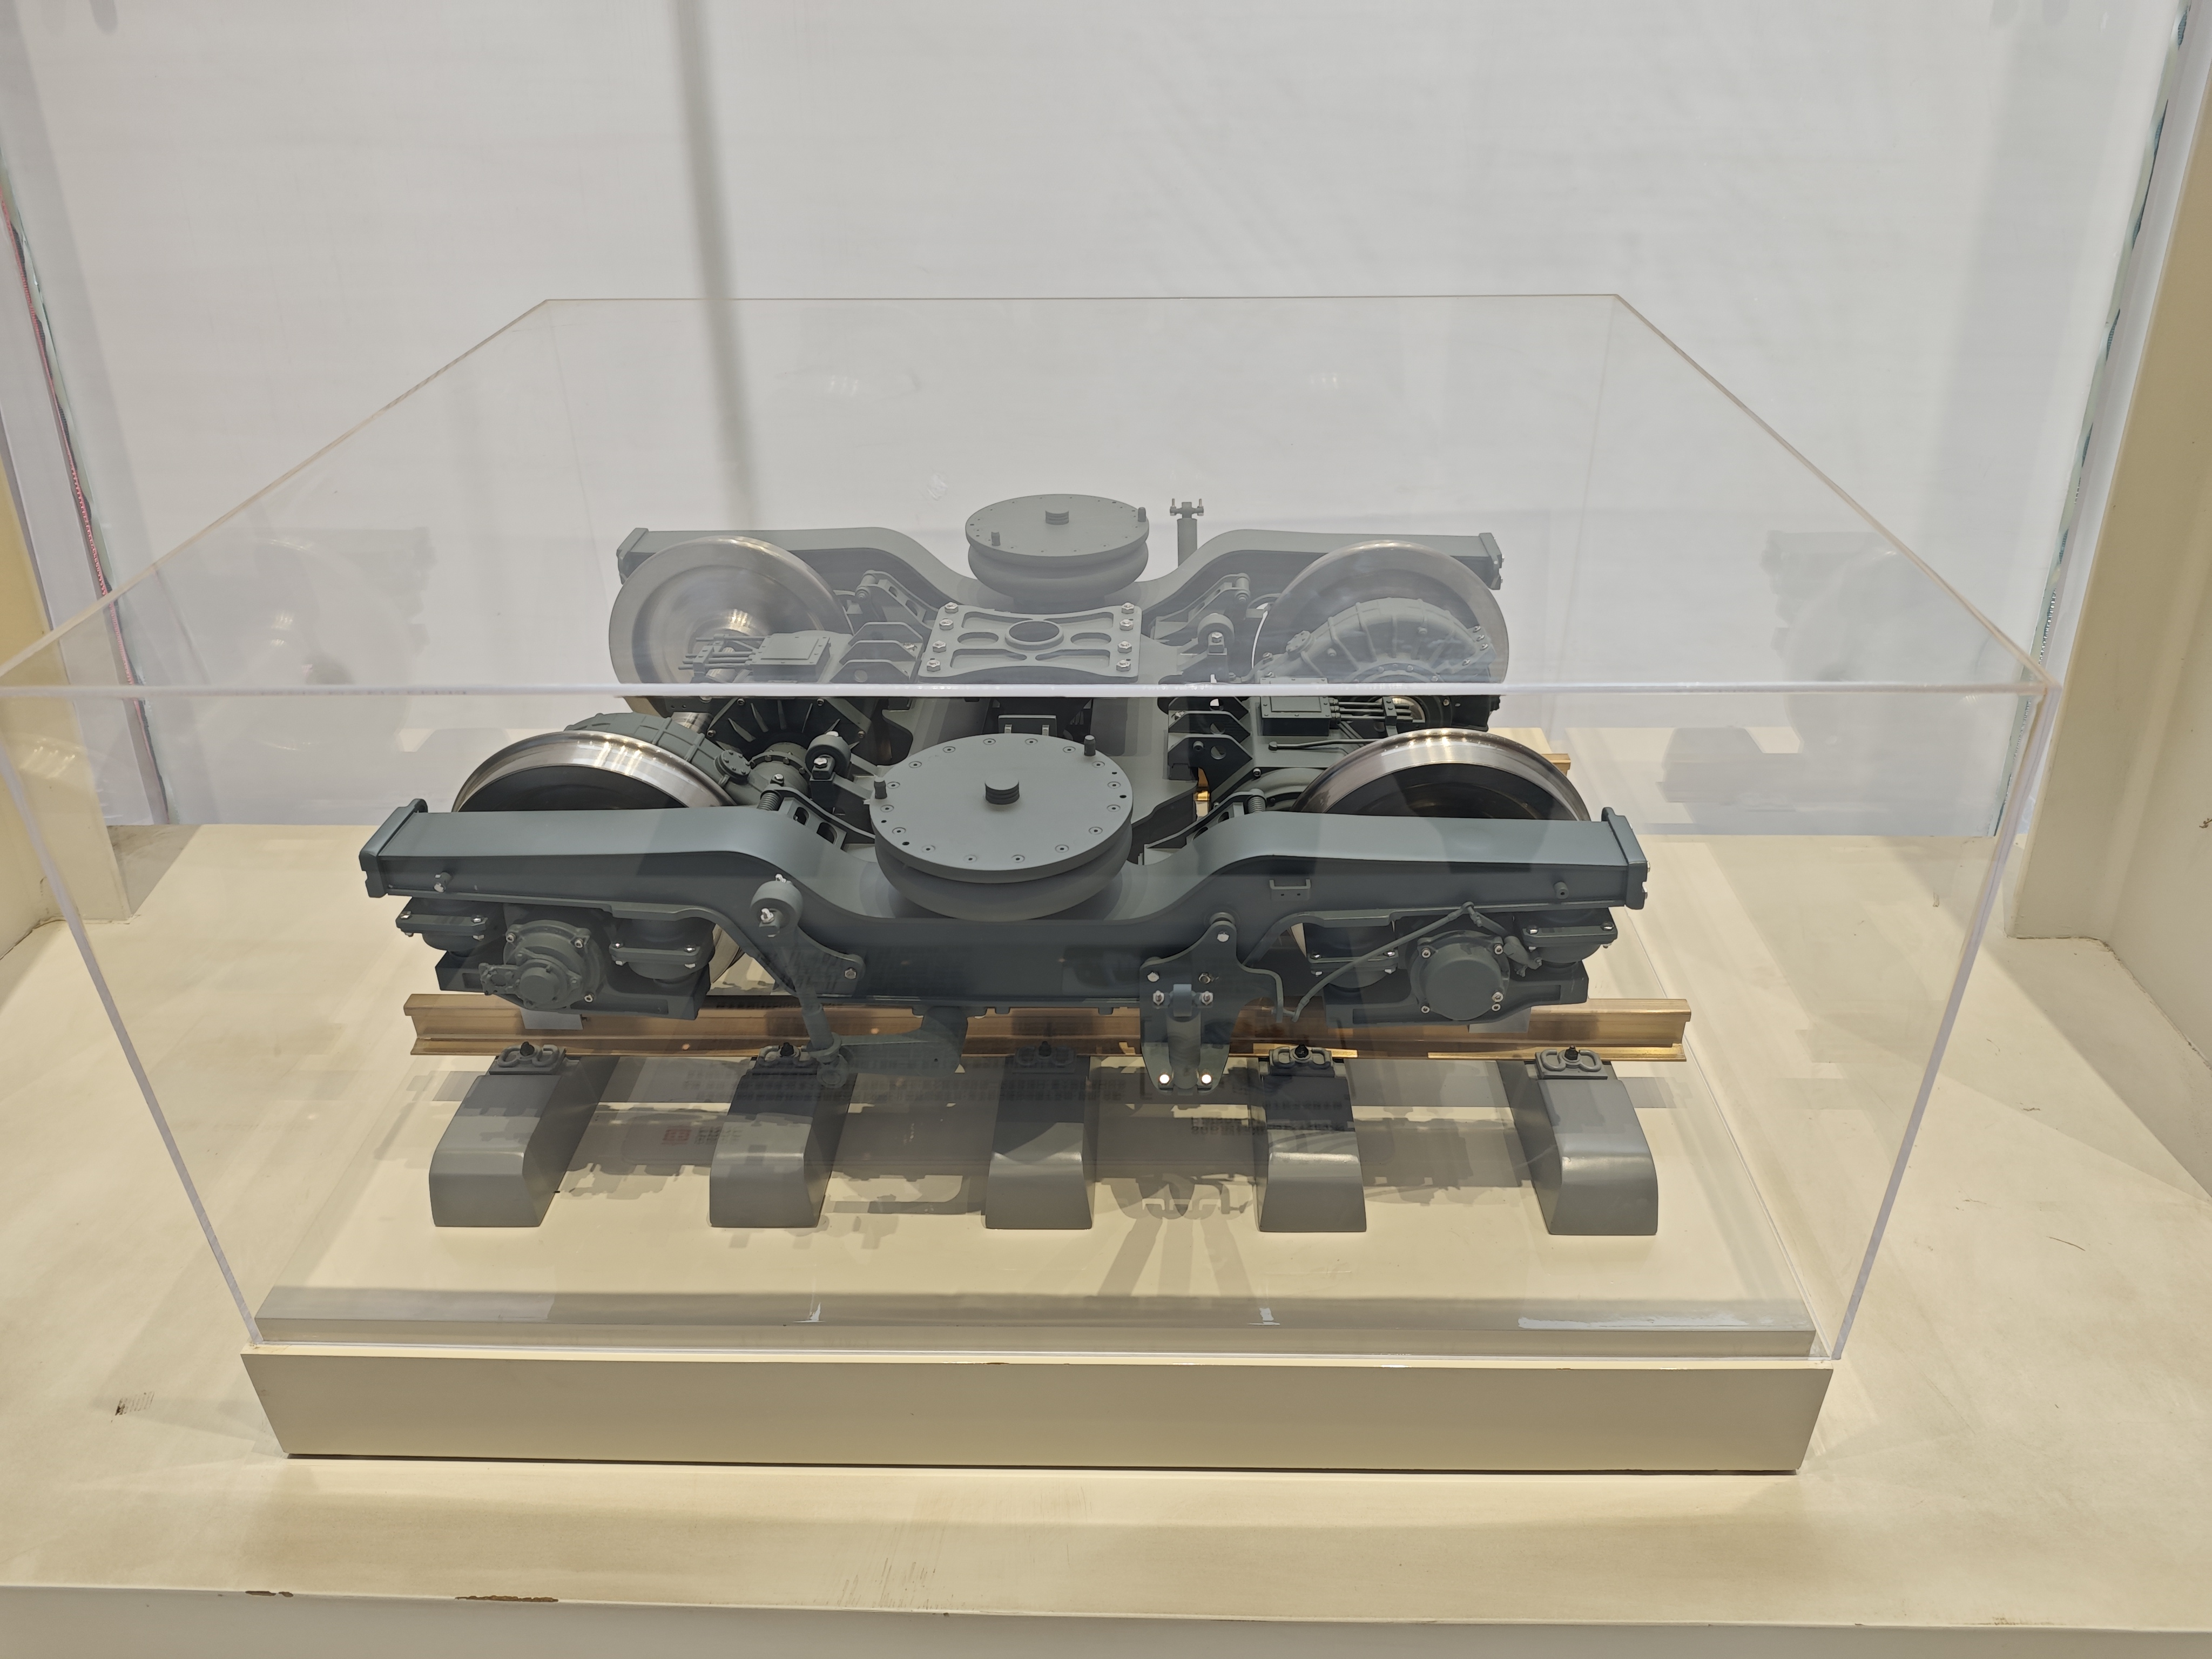
\includegraphics[width=0.8\textwidth]{assets/20260709_122310_2.jpg}
  \vspace{-2.5mm}
  \caption*{\small{}图5\quad{}浦镇产80B型标准地铁转向架PW80E-II}
\end{figure}
\vspace{-7.5mm}\subsection*{二、 转向架分厂参观}\vspace{-2mm}
今天剩下的时间我们去了转向架分厂，了解了转向架组装的工艺。\par{}
\vspace{-5mm}\subsubsection*{2.1\quad{}转向架整体组装}\vspace{-2mm}
转向架组装产线主要有4个工位，分别是节点加装与检测、挂件、落轮和静载/制动性能校验，呈U形排列，如图6：\par{}
\begin{figure}[H]
  \centering
  \vspace{-6mm}
  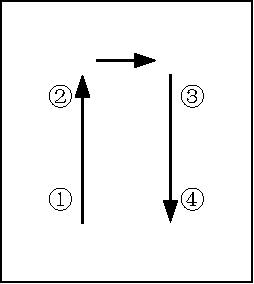
\includegraphics[width=0.25\textwidth, trim=2pt 2pt 2pt 2pt, clip]{assets/U_untagged.pdf}
  \vspace{-8mm}
  \caption*{\small{}图6\quad{}U形生产线示意图}
  \vspace{-5mm}
\end{figure}
第一步顾名思义就是在构架上加装吊挂设备的节点并进行检测；第二步就是指在转向架构架上加装对应部件，如制动缸的闸线，有正位反位两种放置方法，正位对应正常运行时转向架的上下方向，反位则是倒过来，分别用于安装构架上下两边的部件；第三步是指将转向架安装并紧固到轮对上，浦镇厂中的地铁列车一般采用导柱式和转臂式定位；第四步则是做各种力学性能测试。\par{}
厂内运用了很多智能设备，如前一天提到的智能扳手，可以记录员工与对应工作所使用的扭力等相关信息（一个18万）；员工可通过类似手机的手持终端接收任务或上报情况；检查工作时主要采用自检+互检+专检的“三检”模式，转\par{}

\newpage
\journalpage\par\noindent
向架生产线上共有一百多个停止点，当然也有AI检测，但只作最终确认。\par{}
这里AI辅助检测采用了转向架AI机器视觉外观检测技术，采用非接触式、智能化机器视觉技术，通过图片对比找差，识别标记、防锈油是否异常，是否有异物存在，螺栓有无遮挡等，构建多维度精准感知与决策的“AI大脑”。其搭载六自由度机械臂与地沟多向采集模组，实现检测死角全覆盖；采用3D视觉相机，同步触发采集多维度空间图像数据；植入深度学习算法，对海量图片进行网络训练生成预测模型，实时输出精确检测结论。该设备效益十分明显，直接实现了无人化检测（原需要两人），效率提升了$50\%$（$60~\min\to30~\min$），检出率提升了$14\%$（$85\%\to99\%$），并可以自动生成数字化报告，取代了手写纸质报告。\textcolor{gray}{{\bf{}tips: }告示牌原话。}\par{}
当然为了保障国企就业岗位，现阶段是绝对不会大量采用机器替代人工的，仅在部分区域少量应用自动化设备。\par{}
\vspace{-5mm}\subsubsection*{2.2\quad{}轮对制造}\vspace{-2mm}
接着我们又参观了轮对制造产线。轮对是转向架的一个重要组成部分，由轴与轮固结成一个整体，因此轮对制造主要也分为轴和轮两部分。\par{}
首先是轴的制造，先通过车床对毛坯进行粗加工，再通过磨床对轴进行精加工与修正，接着再在一个房间里做探伤检测。\par{}
接着是轮的制造，先对轮饼原料进行加工，再成形打磨其铁屑毛刺等，接着进入预组阶段，即在轮饼与轴接触的内圆上涂抹$\mathrm{MoS_2}$润滑脂方便组装。\par{}
再接着就是正式的压装了，由于轴和轮的接触面呈现一个较为细微的锥度（靠近中轴线的部分宽，反之较窄），同时存在过盈配合，因此可以直接压紧轮与轴。压装好之后还需要进行测量，如测量轮位差等，防止运行时出现跳动等影响舒适性与耐用性的现象。此外还需要进行装盘（轮盘/轴盘式盘形制动）、清洗、装降噪环等步骤，同时对轴和轮分别进行油漆，并在可能松动旋转的位置布置标记。\par{}
厂里摆放着出口到印度班加罗尔的转向架的轮对，由于当地气候原因，甲方要求在轮饼上和轴上都涂油漆；而国内很少在轮饼上涂，一般都只涂在轴上。\par{}
在组装完轮对之后还要进行轴承的压装、轴箱安装等，有单独的车间进行作业。由于该工序对于温度较为敏感，因此为了防止热胀冷缩导致无法安装，要把轮对与轴承存放至该密闭车间在同一温度下保温$8~\mathrm{h}$，因此该车间是恒温的。\par{}
\vspace{-5mm}\subsection*{小结}\vspace{-2mm}
今天还是非常充实的一天，学习到了很多知识。厂里到处都是忙碌的生产线和移动的设备、产品，某些讲解的时候恰好遇上作业进行，十分有现场感。可惜由于保密性质，厂房内无法拍照，否则这次的日记会更加丰富。\par{}

\newpage
\journalpage
\vspace{-7.5mm}
\hypertarget{journal-day-0708}{}
\section*{7月8日\quad{}星期三}
\diaryJournalBodyFont\vspace{-3mm}\par{}
第三天我们首先接着参观了转向架分厂的构架制造部分，然后是车体分厂，最后在总装厂房的培训室进行了实习培训。\par{}
\vspace{-5mm}\subsection*{一、 转向架分厂参观（构架焊接）}\vspace{-2mm}
首先去了转向架分厂，从昨天的学习我们知道转向架除了整体装配和轮对制造，还要进行构架焊接，因此今早主要是参观构架焊接产线，下面是该产线的布局图（其中下图来源于网络\sourcecite{1}，仅大致描绘，可能有部分错误）。\par{}
\begin{figure}[H]
  \centering
  \vspace{-6mm}
  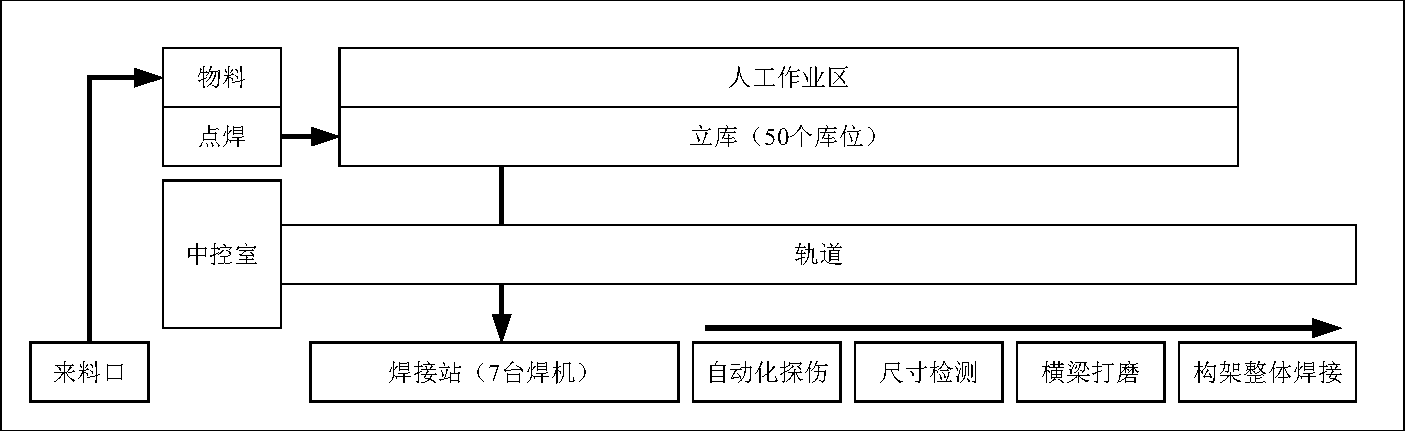
\includegraphics[width=0.98\textwidth, trim=2pt 2pt 2pt 2pt, clip]{assets/GOUJIA_untagged.pdf}
  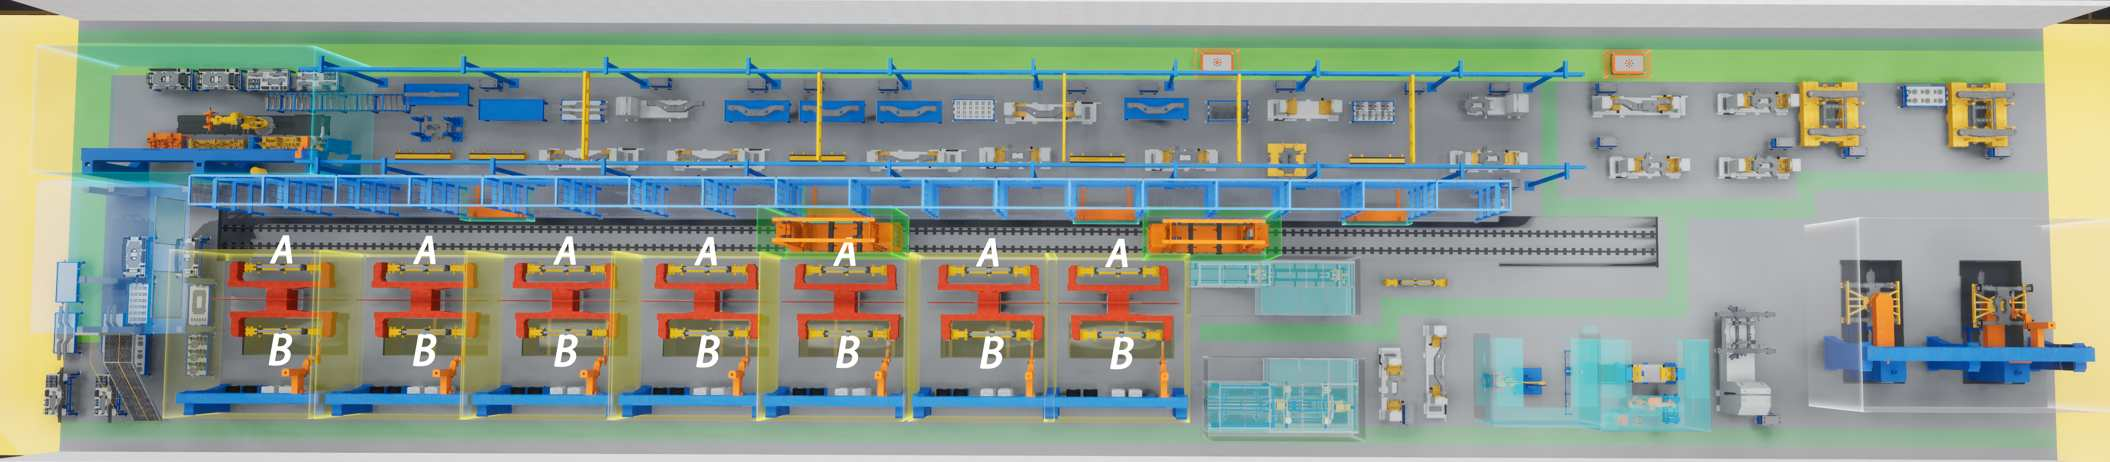
\includegraphics[width=0.96\textwidth]{assets/20260710_120305.jpg}
  \vspace{-2.5mm}
  \caption*{\small{}图7\quad{}构架焊接智能产线示意图}
  \vspace{-5mm}
\end{figure}
大致的焊接流程为：来料口进货，堆放至物料区，并由自动化机器人进行点焊等装配工序；初步装配后由AGV运送至立库或焊接站，由7台焊接机器人进行焊接（操作仅需2人），焊接后进行磁粉探伤、尺寸检测、打磨等步骤，并进行整体焊接（可能记错了？）；期间会有AGV小车穿梭于机器与立库之间运送物料。如果设备发生异常，系统会第一时间通知一线工人，同时报警信息也会传送至中控室的数字孪生界面，方便工人或管理者进行修复。\par{}
\vspace{-5mm}\subsection*{二、 车体分厂参观}\vspace{-2mm}
接着我们参观了车体分厂。这个厂由于有机器出现故障，因此今天生产暂停，可惜没能观摩生产过程。该厂共有B03、B04、B05三条全铝合金焊接线，绝大多数采用自动焊接的方式进行，仅有部分小件焊接需要人工完成。\par{}
其中较具有代表性的就是铝合金搅拌摩擦焊技术，原理就是高速旋转的搅拌头与工件摩擦产生热量，使得材料热塑性化，搅拌头沿着待焊界面移动，促使热塑性材料在搅拌头作用下相互扩散、混合，进而实现固态连接。该技术具有绿色环保、高效率、变形小、强度高等优势。\textcolor{gray}{{\bf{}tips: }告示牌原话。}\par{}

\newpage
\journalpage\par{}
此外还有车体底架尺寸自动化检测技术，采用结构光三维视觉检测技术，通过生成点云实现非接触式测量。可用于底架加工完成后100多个尺寸检测顶点的快速精确检测，直接实现了无人化检测（原需要两人），效率提升了$50\%$（$30~\min\to15~\min$），精度提升了$98\%$（$0.5~\mathrm{mm}\to0.01~\mathrm{mm}$），同时也可以自动输出检测记录。\textcolor{gray}{{\bf{}tips: }告示牌原话。}\par{}
还有前几天提到的底架激光投影定位技术、铝合金氧化膜自动化激光清洗技术等，此处不再赘述。上述各种高新技术的运用均减少了人工使用量、提升了工作效率并增加了工作准确率，适合浦镇厂小批量、多品种的制造特点。\par{}
\begin{figure}[H]
  \centering
  
\includegraphics[width=0.8\textwidth]{assets/20260710_124933_mosaic_big_q50.jpg}
  \vspace{-2.5mm}
  \caption*{\small{}图8\quad{}参观途中遇到的神必黄车}
  \vspace{-2.5mm}
\end{figure}
\vspace{-5mm}\subsection*{三、 总装实习理论教育}\vspace{-2mm}
最后我们来到隔壁的总装分厂，进行简单的培训。\par{}
\vspace{-2mm}\subsubsection*{3.1\quad{}安全教育}\vspace{-2mm}
大门不开，只走车，人要走旁边小门；走路不要看手机分神，手机不要拍照；安全帽要戴好，防止碰头；高站流水线上楼梯要扶扶手，间隙不要踩空；车内线束、支架等注意避让，防止碰伤或摔倒；配送车、天车要注意避让，做到人让车；垃圾要扔到蓝色垃圾桶。\par{}
\vspace{-5mm}\subsubsection*{3.2\quad{}管理方面}\vspace{-2mm}
总装厂作为制造单元之一，是浦镇四大分厂中最大的；四大分厂是车体分厂、转向架分厂、总装分厂和修理分厂，其中修理分厂在老厂区，其他均在新厂\par{}

\newpage
\journalpage\par\noindent
区。总装分厂由原来的总装车间与客车车间合并而成；客车车间中的修理部分即变为修理分厂，新造部分即合并至总装分厂。\par{}
管理上主要分为三个业务组：生产管理组、技术质量组、综合管理组等，分管不同方面。\par{}
\vspace{-5mm}\subsubsection*{3.3\quad{}生产方面}\vspace{-2mm}
新厂区高峰期4辆/日，老厂区$4\sim6$辆/日（4新造+2维修），新厂区的量产车一车每日走2个工位，一周即可走完全部14个工位。\par{}
总装完毕后还需要进行跑车试验等；此外厂房分为$300~\mathrm{m}\times60~\mathrm{m}$或$300~\mathrm{m}\times42~\mathrm{m}$两种尺寸。\par{}
\vspace{-5mm}\subsubsection*{3.4\quad{}工艺流程方面}\vspace{-2mm}
首先是工艺布局，大致如下图：\par{}
\begin{figure}[H]
  \centering
  \vspace{-6mm}
  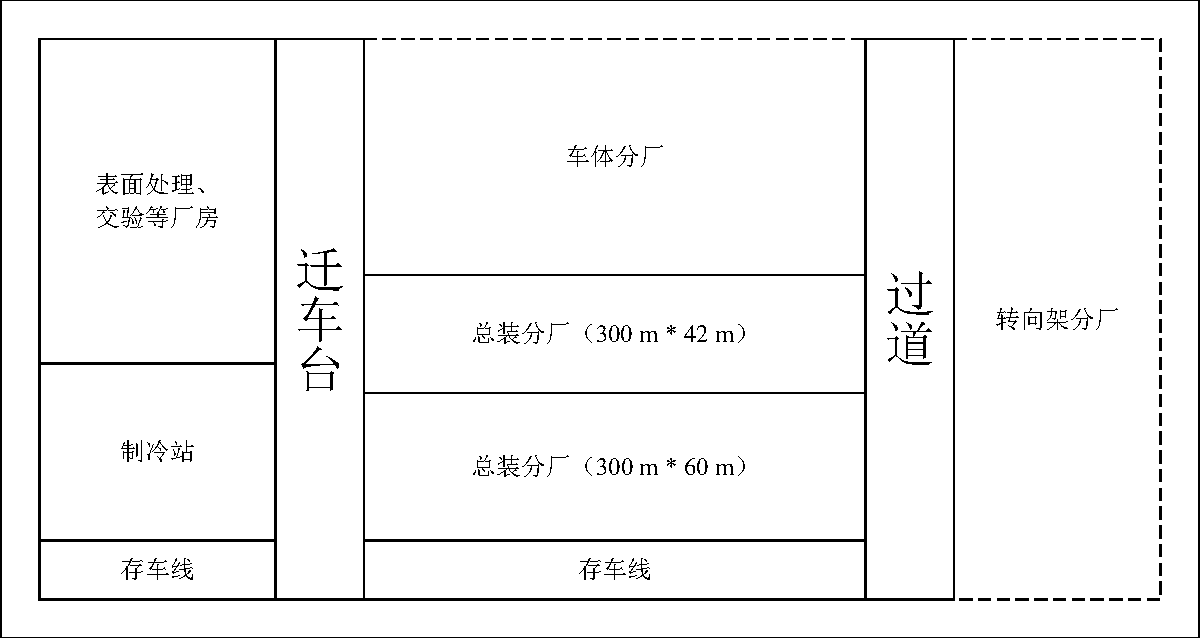
\includegraphics[width=0.8\textwidth, trim=2pt 2pt 2pt 2pt, clip]{assets/MAP_untagged.pdf}
  \vspace{-5mm}
  \caption*{\small{}图9\quad{}总装厂房位置布局（简化）}
  \vspace{-5mm}
\end{figure}
接着讲了车辆构成和工艺流程（课内或前几天基本已了解，略过）。\par{}
\vspace{-5mm}\subsubsection*{3.5\quad{}质量管理方面}\vspace{-2mm}
“质量”意味着“满足要求”，“要求”就是说明书、作业指导书里的要求。\par{}
影响质量的六个要素为：人、机、料、法、环、测，即人为因素、机械因素、原料因素、方法因素、环境因素、测试因素等，最主要的一定是人。\par{}
为了保证质量，要遵循“三不”原则：不接受、不制造、不传递不合格品。\par{}
遇到问题应做到六字诀：停止、呼叫、等待，把问题向上报告，将信息从作业者依次传递给工位长、工区长，不能隐瞒或擅自行动。\par{}

\newpage
\journalpage
\vspace{-7.5mm}
\hypertarget{journal-day-0709}{}
\section*{7月9日\quad{}星期四}
\diaryJournalBodyFont\vspace{-3mm}\par{}
今天去总装分厂观摩学习，主要是在$42~\mathrm{m}$跨的厂房里的高站流水线上。我们分到的工位当天在准备对上海地铁21号线列车进行$5~\mathrm{kV}$耐压测试。该车以黑色打底，白色、橙色、金色波浪线横贯车体，图案十分有动感；整车采用内藏式车门，开门时门缩入墙体内。当然只有我们那一个工位上的车厢有彩绘，其他的还只有黑色底，没有图案。\par{}
带队的工人师傅说，因为上海地铁要求实现的功能较为丰富，因此该型列车的设备较多。由于工人师傅比较忙，我们就没有去打扰他们，自主进行观察，偶尔提问。\par{}
我们登上高站，进入列车进行观察，列车内装还没完全安装好，很多线缆还垂在外面，密密麻麻的线缆都要一根根连接，十分复杂；座位下也有一些设备，但也还没安装。\par{}
我们参观的是$\mathrm{M_p}$车，一般是4动2拖编组的第2、5节，和$\mathrm{T_c}$车的区别一是没有驾驶室，二是多了牵引逆变器等设备；和$\mathrm{M}$车的区别就是多了三位开关，可以切换至受电弓、车间电源与地三个挡位；当然该车三位开关写了受电弓这几个字，自然是受电弓+接触网受流而不是集电靴+第三轨，只不过受电弓还没安装。\par{}
后来我又去其他工位了解了一下车下设备的情况，图10是我根据实际情况绘制的$\mathrm{M}$车车下设备的布局图：\par{}
\begin{figure}[H]
  \centering
  \vspace{-6mm}
  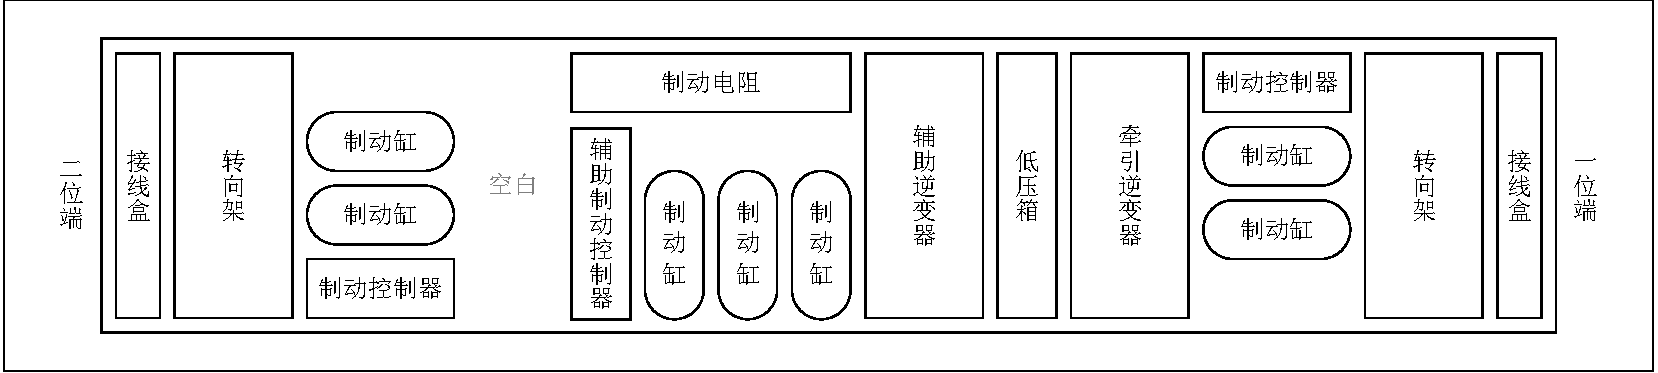
\includegraphics[width=0.98\textwidth, trim=8pt 2pt 8pt 2pt, clip]{assets/M_untagged.pdf}
  \vspace{-5mm}
  \caption*{\small{}图10\quad{}上海地铁21号线M车车下设备布局图}
  \vspace{-5mm}
\end{figure}
由图可得，该车又有制动电阻又有制动缸，说明该车制动是采用电阻制动加空气制动的形式；其中一般现代地铁的空气制动大都用电信号控制制动机。而从前几天的转向架分厂学习的知识可得，浦镇厂生产的列车大都是使用盘形制动，盘形制动又分为轮盘式和轴盘式，地铁多用轮盘式。\par{}
和学校里的1动1拖编组的试验车相比，这节车厢的$\mathrm{M}$车直接自带了一个辅助逆变器和低压箱，而学校里的试验车的辅逆安装在$\mathrm{T_c}$车上。值得注意的是靠近二位端的电空制动装置旁边存在着一片未安装设备的区域，不明确是否有设备暂时没安装。\par{}
此外，由铭牌可得$\mathrm{M}$车上的辅助逆变器、低压箱、牵引逆变器，以及$\mathrm{M_p}$车上的高压箱基本都是上海阿尔斯通公司生产的，可见该公司业务的广泛。\par{}

\newpage
\journalpage\par{}
车下的电气设备上一般都写了以下几行字：\par{}
\begin{center}
  \setlength{\fboxsep}{7pt}
  \fbox{
    \begin{minipage}{0.6\textwidth}
      \diarySong\fontsize{12pt}{13.5pt}\selectfont
      \noindent{\bf{打开箱盖之前：}}
      \vspace{-2mm}
      \begin{enumerate}
        \setlength{\itemsep}{0pt}
        \setlength{\parsep}{0pt}
        \setlength{\topsep}{2pt}
        \setlength{\partopsep}{0pt}
        \item 降下所有受电弓；
        \item 断开所有车间电源；
        \item 等候$5~\min$；
        \item 将所有的IES开关锁定至“接地”位置。
      \end{enumerate}
    \end{minipage}
  }
\end{center}
这个是供检修用的，为保证维修人员的安全，要求断电、三位开关接地、电荷通过放电电阻释放完毕等，所以会有这些要求。\textcolor{gray}{{\bf{}tips: }依旧是上牵引控制课讲过的内容……}\par{}
同时，我们参观时迁车台还进行了迁车作业，是拿一台公铁两用的小拖拉机把车厢拖到迁车台上进行平移换轨的，十分新奇。\par{}
总之，今天看了很多东西，也复习了一下课上所学知识，感觉还是很有意义的。\par{}

\newpage
\journalpage
\vspace{-7.5mm}
\hypertarget{journal-day-0710}{}
\section*{7月10日\quad{}星期五}
\diaryJournalBodyFont\vspace{-3mm}\par{}
今天上午继续在总装分厂进行观摩学习。\par{}
早上7:50，我们和工人们一起开了晨会，我所在的工作组简单交代了一下任务就开始干活了。我还是回到了我昨天待的工位上，结果发现好像昨天那节已经涂装好的车厢已经迁移到旁边的轨道上了，而人是跟着任务走的，所以今天我所在的工位好像有人员变化。\par{}
今天主要就是四处转转，除了上海地铁21号线列车，在厂房内的列车还有杭州地铁、穗莞深城际，以及出口至沙特阿拉伯的跨座式单轨、出口至格鲁吉亚第比利斯的地铁列车等，有点小差异，各有各的美。\par{}
印象最深的就是穗莞深城际列车，整体远看像国铁的动车组，近看像大地铁，车身是银白色的，有类似于和谐号的横条纹，只不过条纹是紫色；每节车厢有前中后三个车门，和地铁的五个车门、一般国铁客车或动车组车厢的两个车门都不一样；此外车下的电气设备也使用外壳进行了包裹，而地铁列车是没有的，非常整齐美观。\textcolor{gray}{{\bf{}tips: }我过几年高低得坐一坐这条线……}\par{}
而沙特单轨车的头车停在角落里，是纯白色，车窗上沿有可变色的灯带，主打一个简约。路过的时候正好在调试灯光，前面车灯全部打开了，驾驶室上方的LED横幅也在滚动显示信息，有英语和阿拉伯语两种显示（滚动方向是反的），回想前几天不知在哪个环节听到的描述，推断这就是出口至沙特的单轨。\par{}
下午我们简单了解了浦镇公司的业务发展史，其核心业务就是轨道交通装备业务，支柱业务是运营、维保、修理等延伸业务，支撑业务是智能制造、智能产品、智能运营等新产业业务。\par{}
同时还了解了一下职业生涯的发展通道，一般新员工经过一年左右的磨合，可以选择两条通道，一条是行政管理通道，另一条是专业技能通道（即管理岗和技术岗）；招聘技术人员以校招为主，共分为$\mathrm{L1}\sim\mathrm{L10}$这十个等级，一般校招进来的技术人员都是$\mathrm{L8}$或$\mathrm{L9}$级，后面每2或3年进行评级。\par{}
后面还讲了薪酬福利体系，其实光从伙食就可以看出福利其实已经非常不错了，此外还有各种补贴，确实很符合我对国企的印象。\par{}
最后还邀请了老学长进行分享，大家热情地交流后，在浦镇厂的实习就迎来了尾声。\par{}
总的来说这五天非常充实，从技术到管理，我们了解了很多关于列车制造的知识，同时也温习了我们学习的课内知识，还了解了浦镇厂的一些细节，这也是学习生涯中不可多得的实践机会。\par{}

\newpage
\journalpage
\vspace{-7.5mm}
\hypertarget{journal-day-0713}{}
\section*{7月13日\quad{}星期一}
\diaryJournalBodyFont\vspace{-3mm}\par{}
今天我们来到了位于上海市嘉定区安亭镇伊宁路2620号的申通中车轨道交通车辆有限公司，也就是上海赛车场车辆段，下图为其在配线图中的位置\sourcecite{2}与其外景；其从上海赛车场花桥方向的交叉渡线两端引出轨道并抬升至地面，可直接通向车辆段车库（棕色方块处），或经折返后进入综合维修中心（红框处）。我们今天参观的就是红框处的维修中心。\par{}
\begin{figure}[H]
  \centering
  \vspace{-1.5mm}
  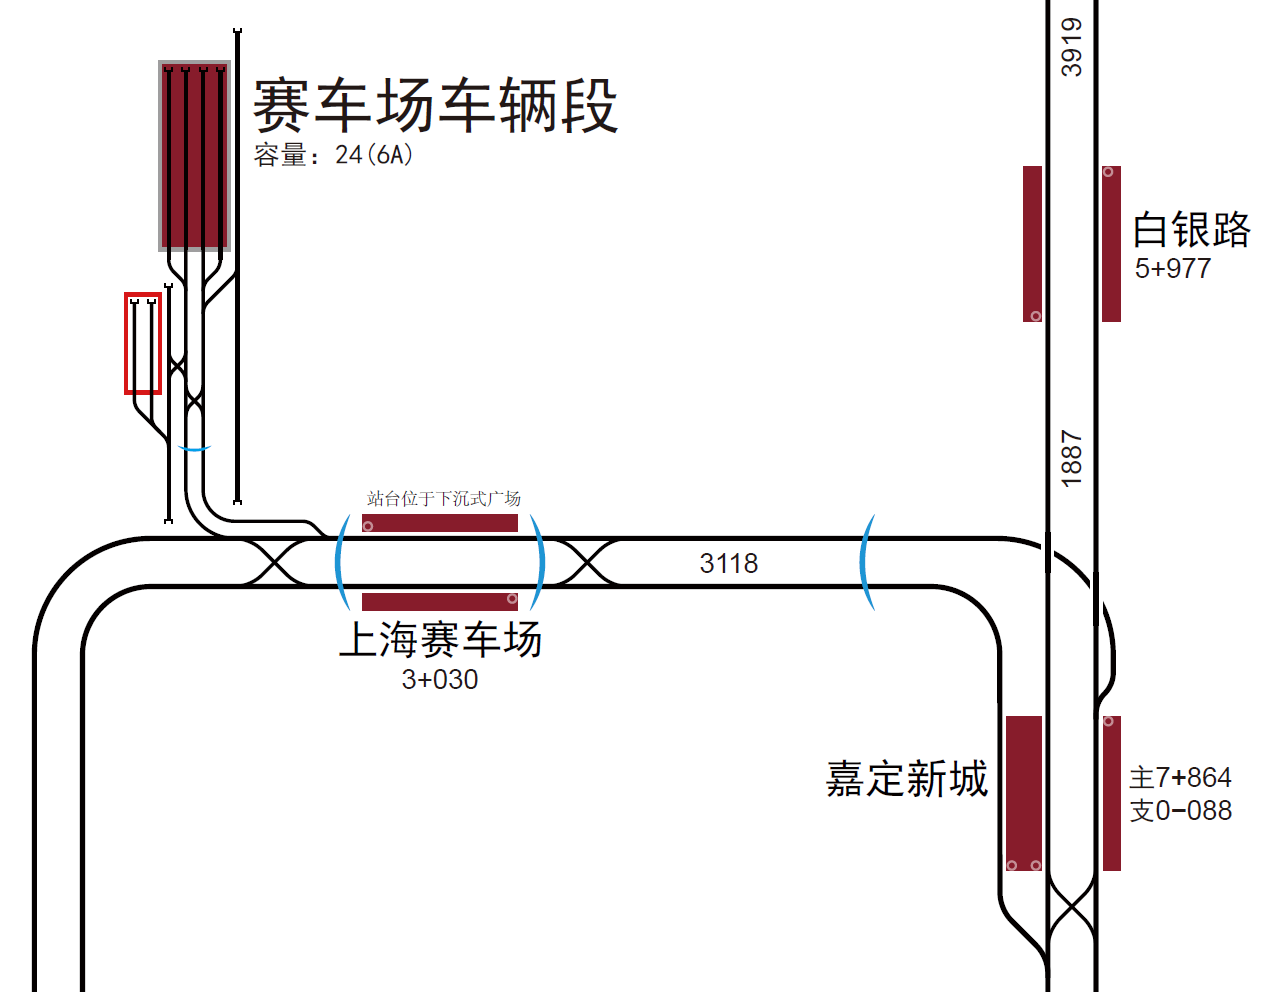
\includegraphics[width=0.48\textwidth]{assets/day6.png}
  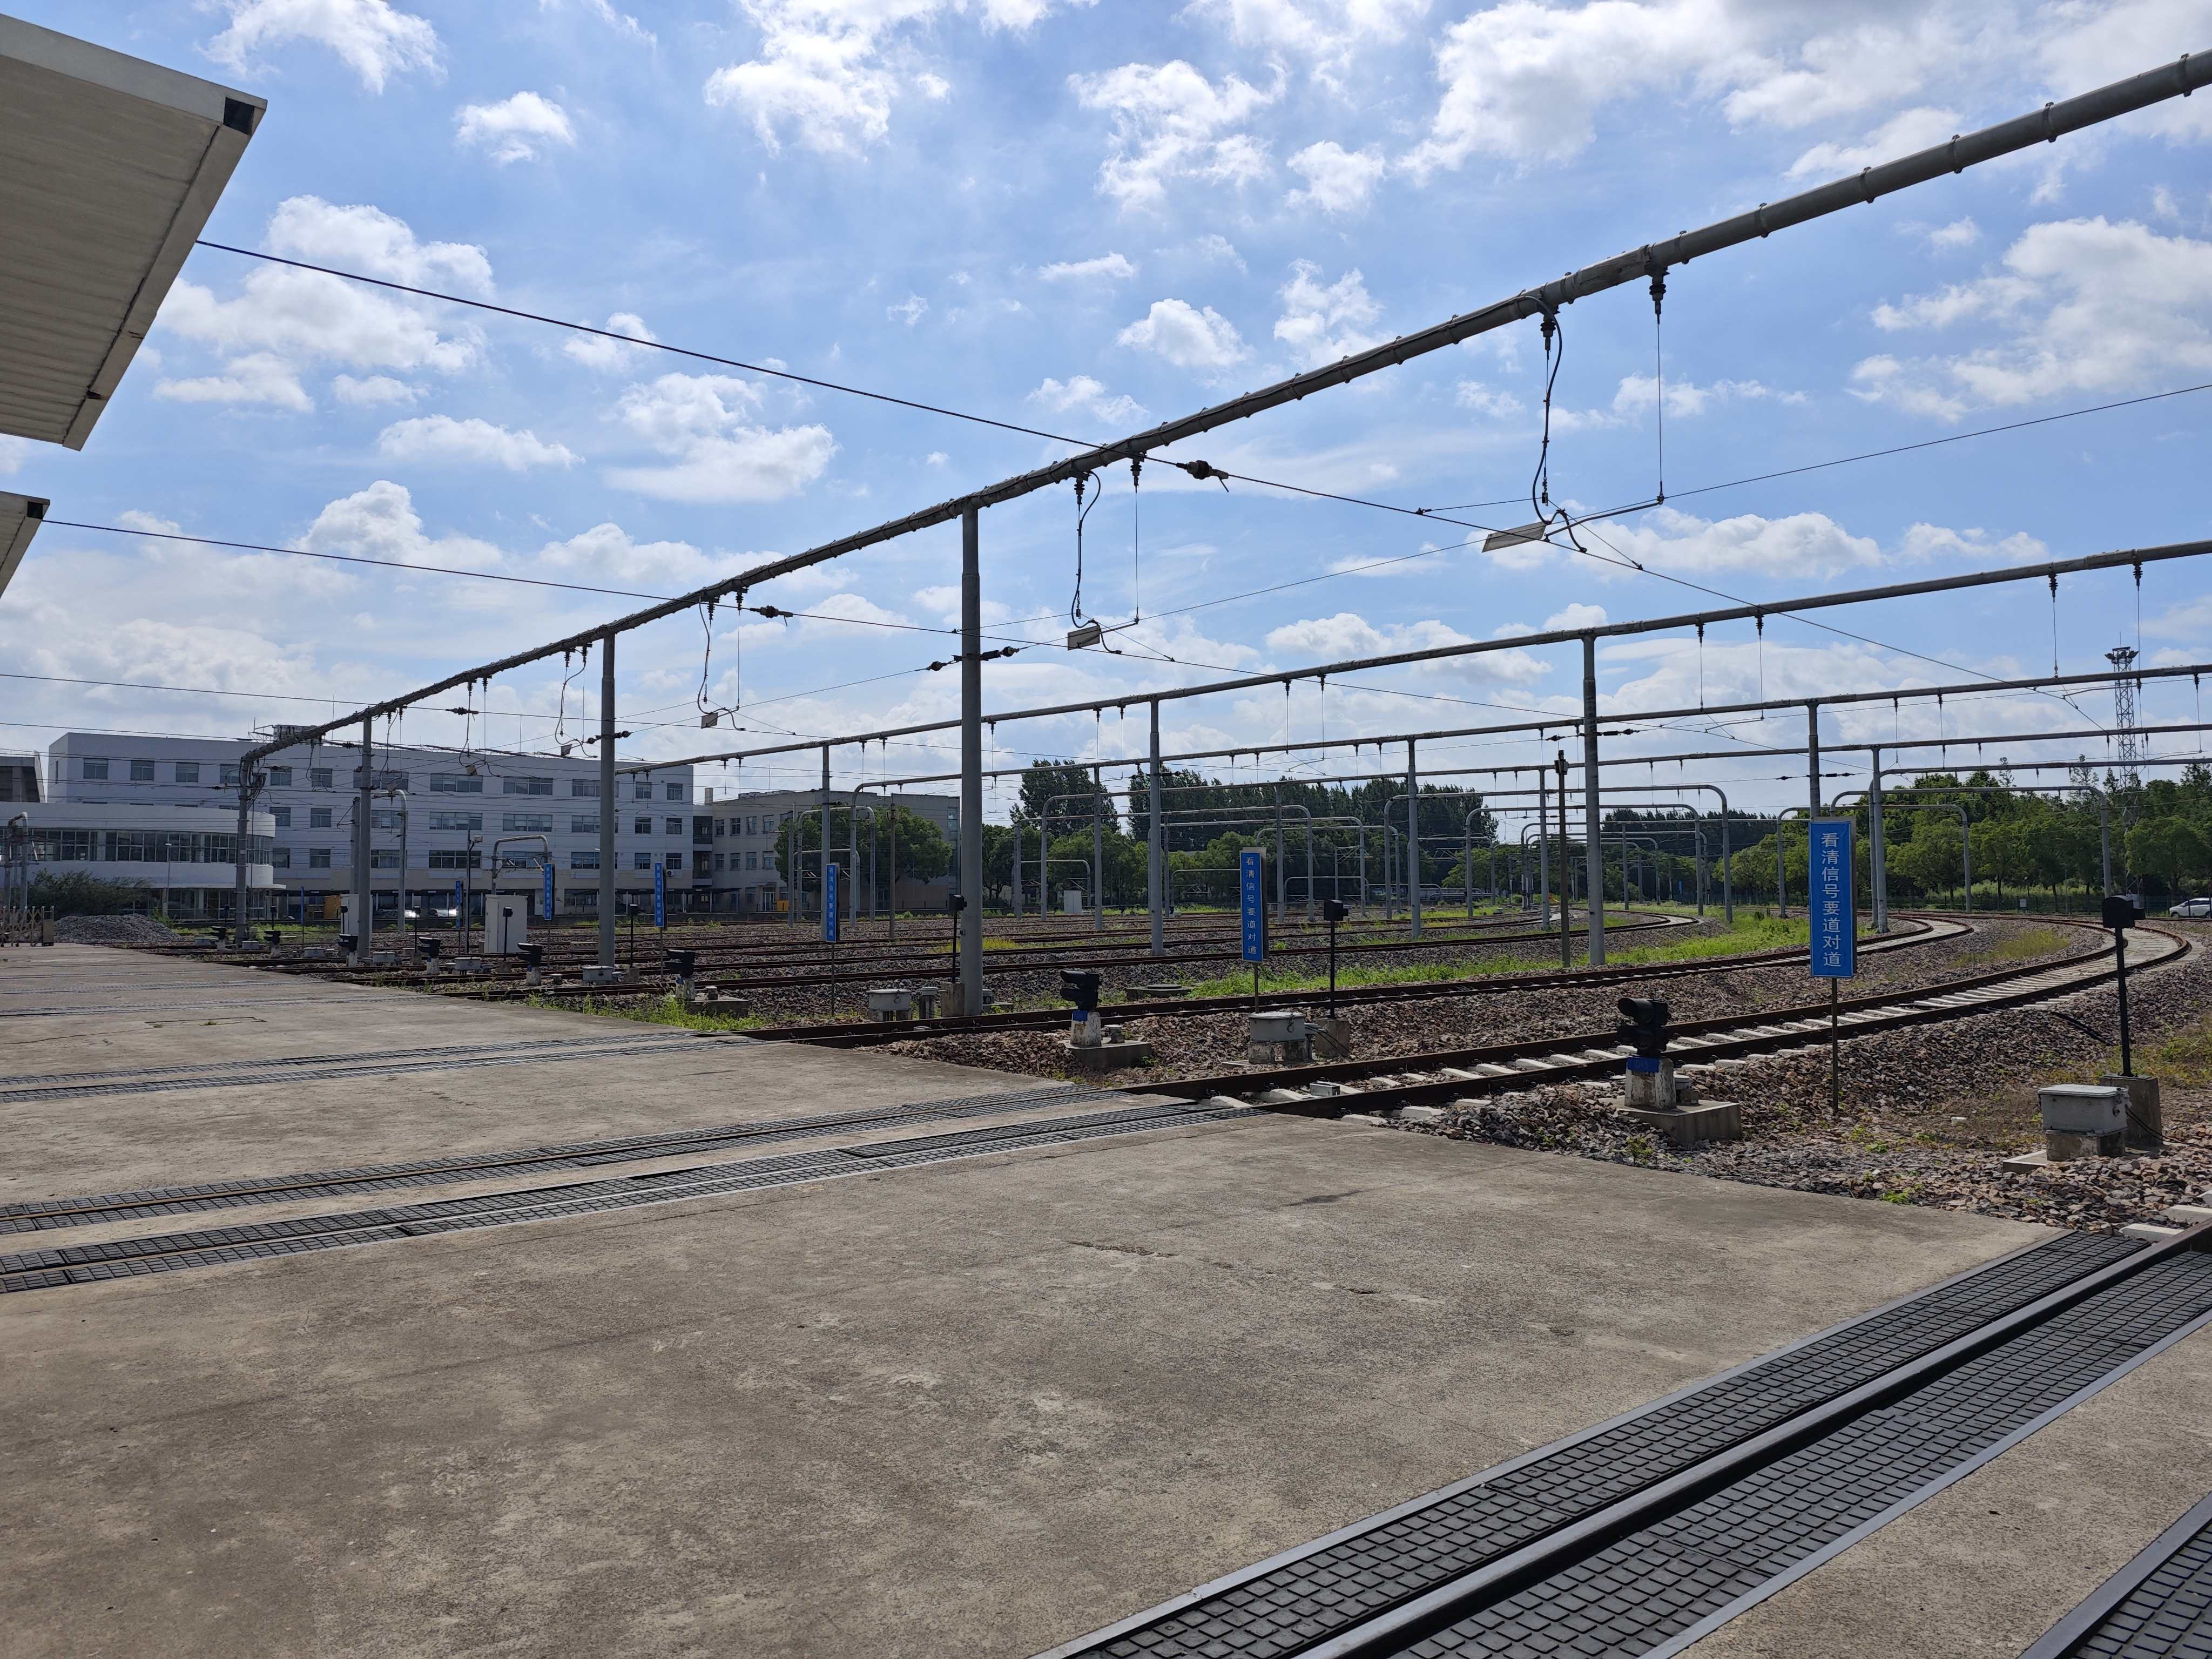
\includegraphics[width=0.5\textwidth]{assets/20260716_233131.jpg}
  \caption*{\small{}图11\quad{}上海赛车场车辆段位置与概况}
  \vspace{-5mm}
\end{figure}
该维修中心主要承担上海11号线的修缮维护工作，主要由总体拆卸、车体设备维护、转向架拆卸与维护、轮对拆卸与维护、电机维护、各部件到总体依次组装的过程构成。我们在车间内看到了大量转向架或构架，如下图的灰色构架和铁锈色转向架，属于11号线或16号线的列车。\par{}
\begin{figure}[H]
  \centering
  \vspace{-1.5mm}
  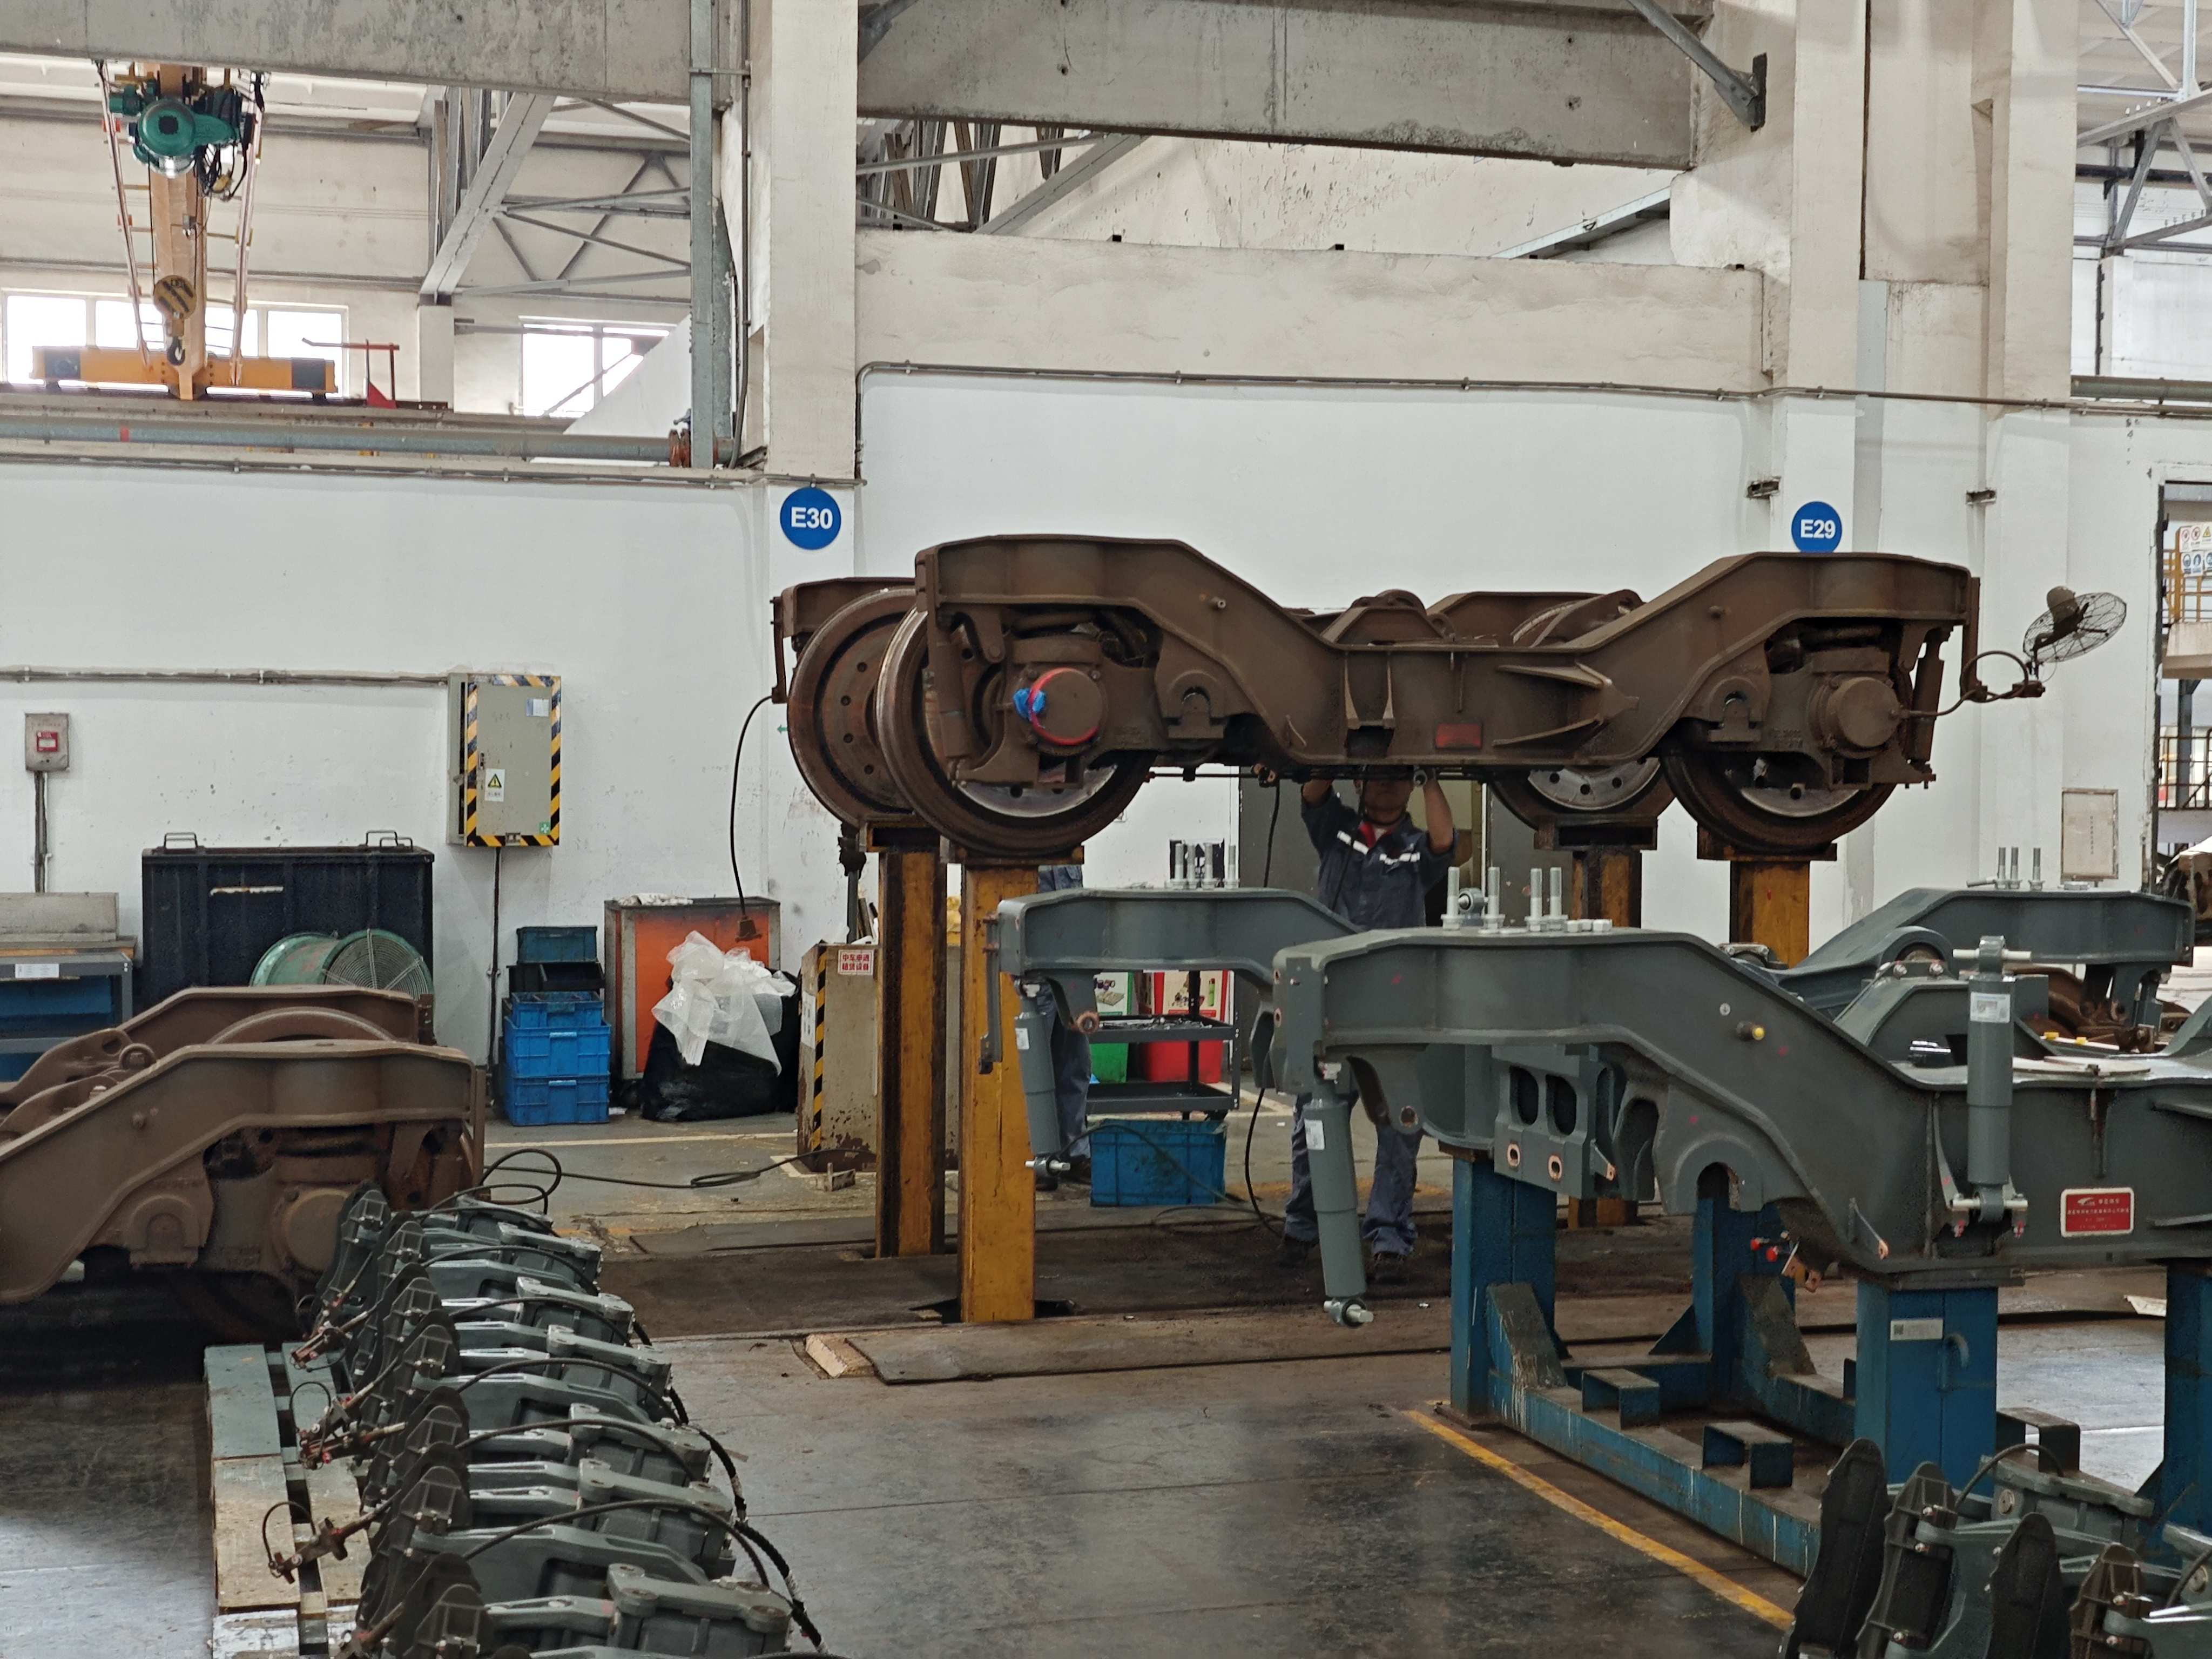
\includegraphics[width=0.8\textwidth]{assets/20260717_034156.jpg}
  \vspace{-2.5mm}
  \caption*{\small{}图12\quad{}转向架拆卸}
\end{figure}

\newpage
\journalpage\par{}
其中有一个转向架正在架车台上进行拆卸工作。隔壁车间存放着很多列车的车体，目测以11号线列车居多，这里暂且不做展示，见后文。\par{}
图13左展示的是一系悬挂钢弹簧，可见其分为内外两圈且旋向相反，目的是增大空间利用率并防止弹簧穿插卡顿；右图展示的是拆卸下来的轮对，可见其轴上偏右的位置有一个齿轮箱，这和我们在浦镇公司看到的新造轮对基本一致。\par{}
\begin{figure}[H]
  \centering
  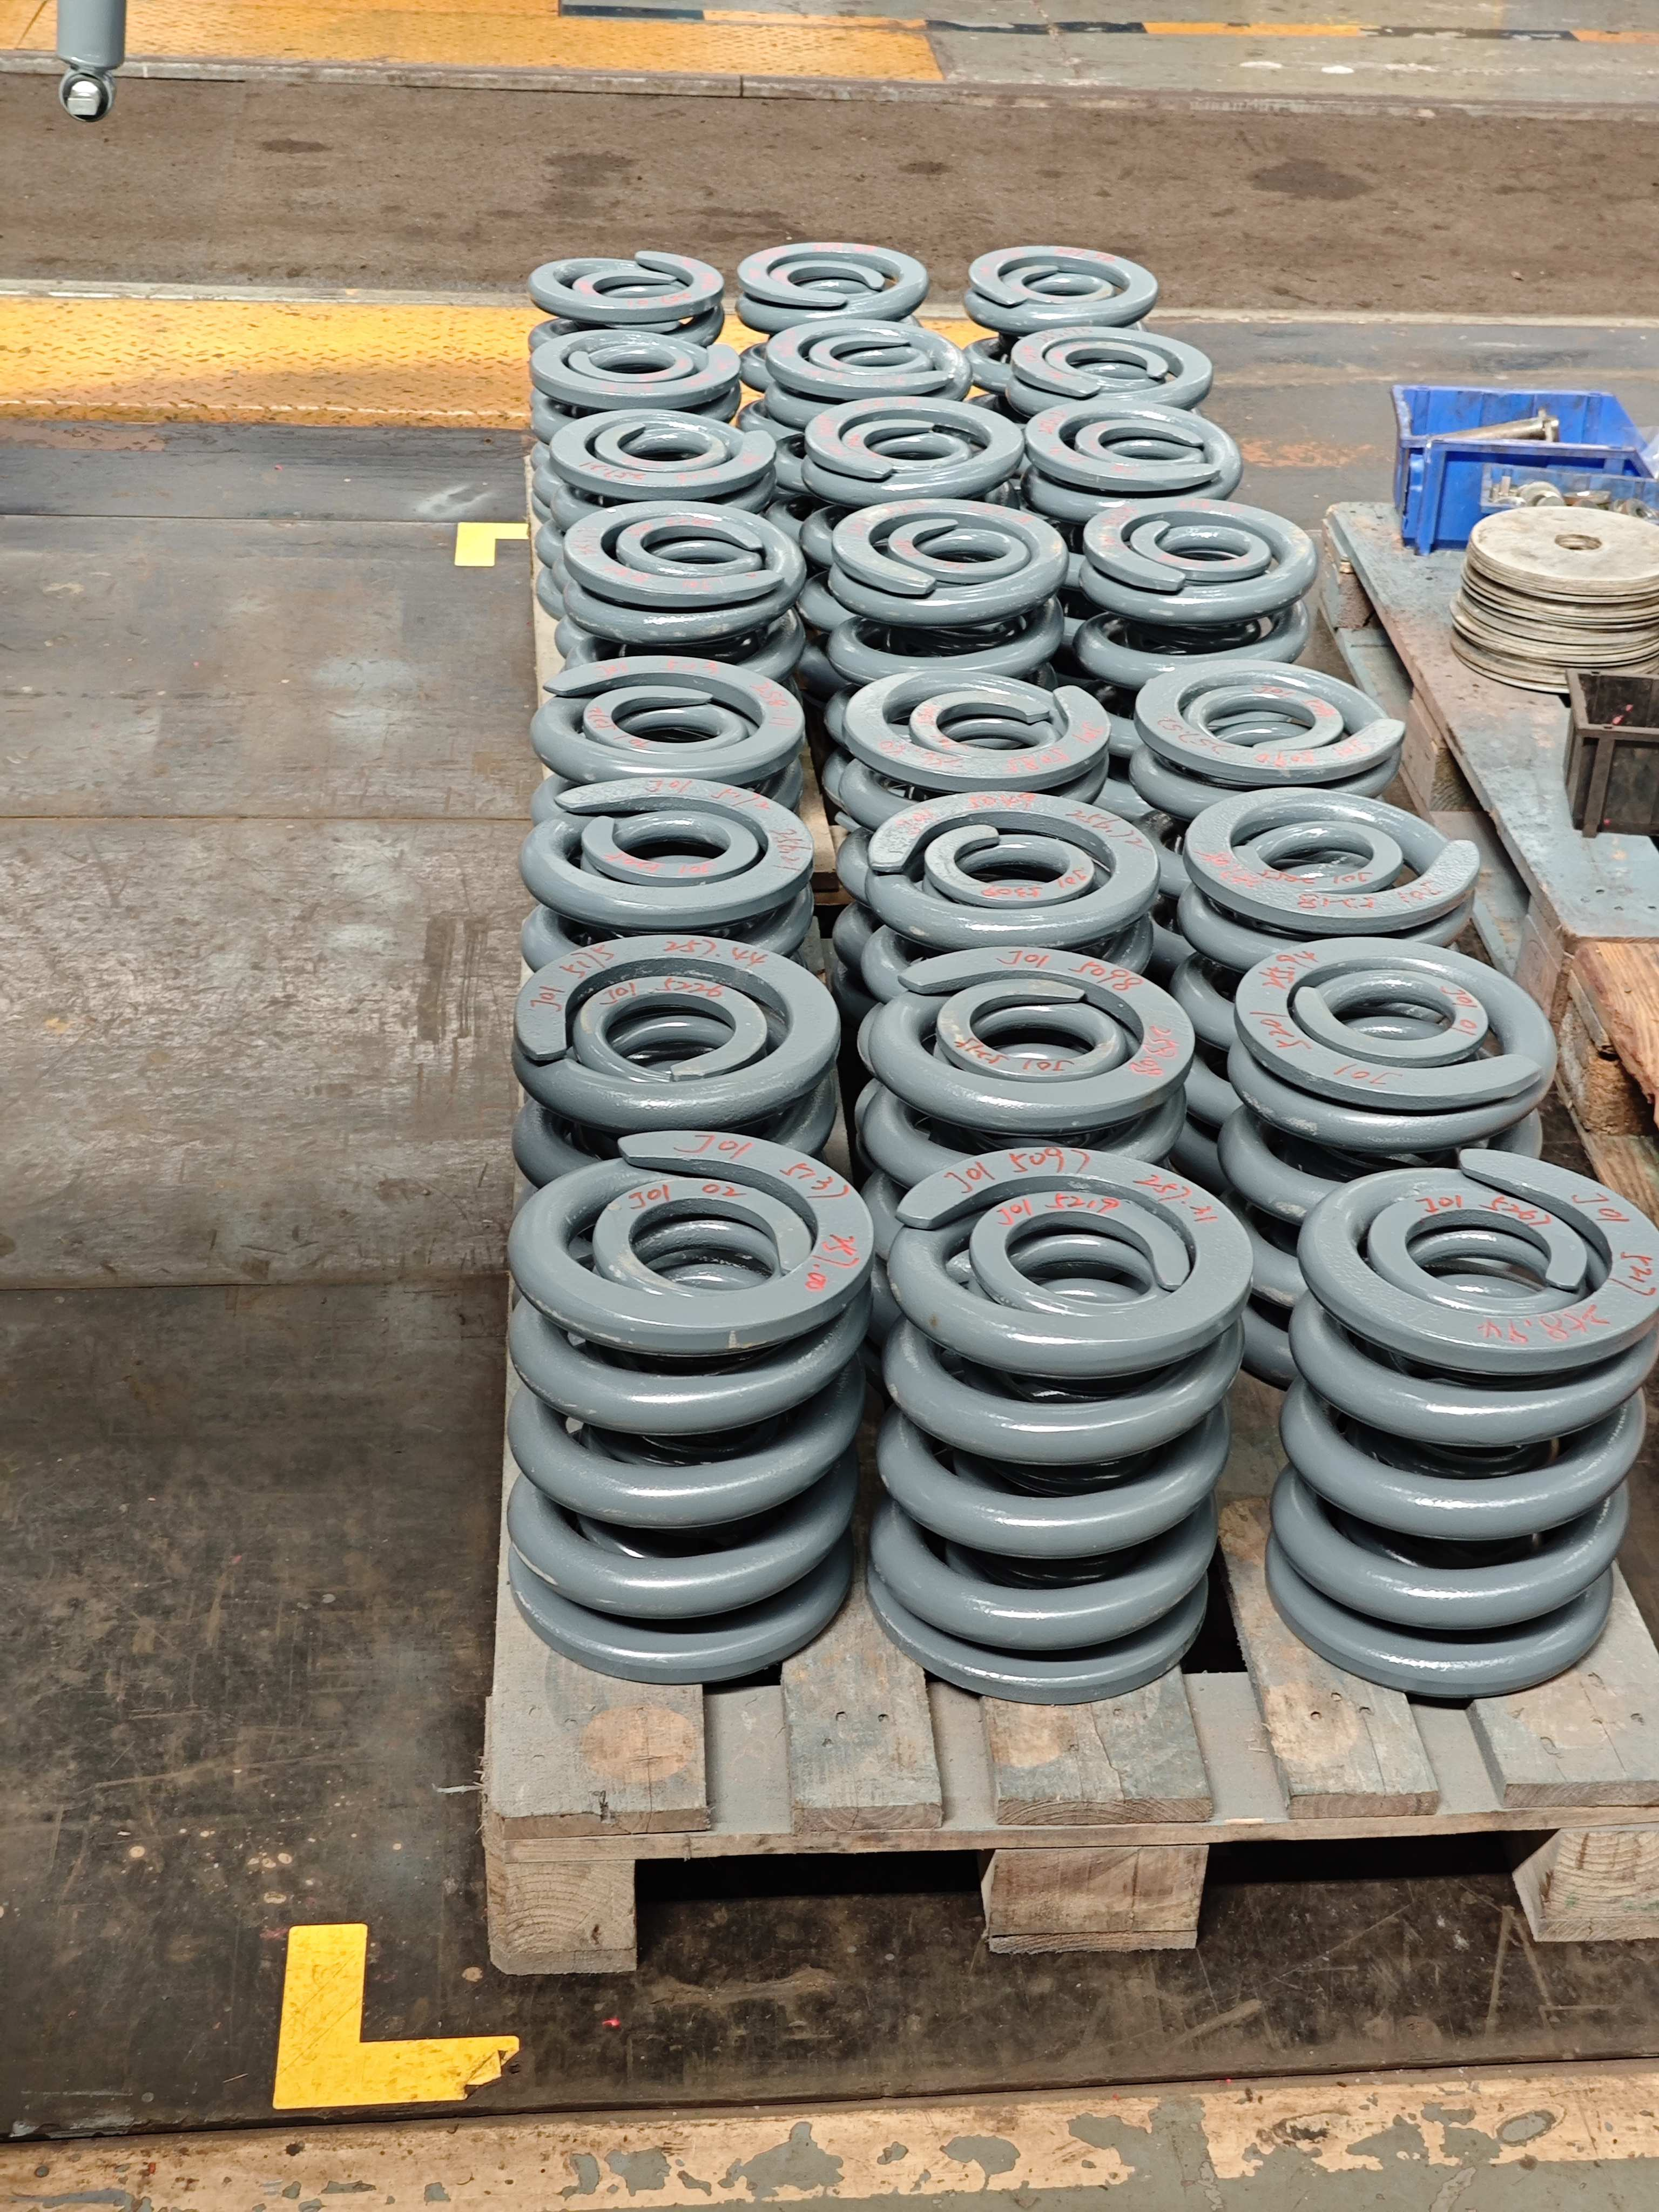
\includegraphics[width=0.45\textwidth]{assets/20260717_034823.jpg}
  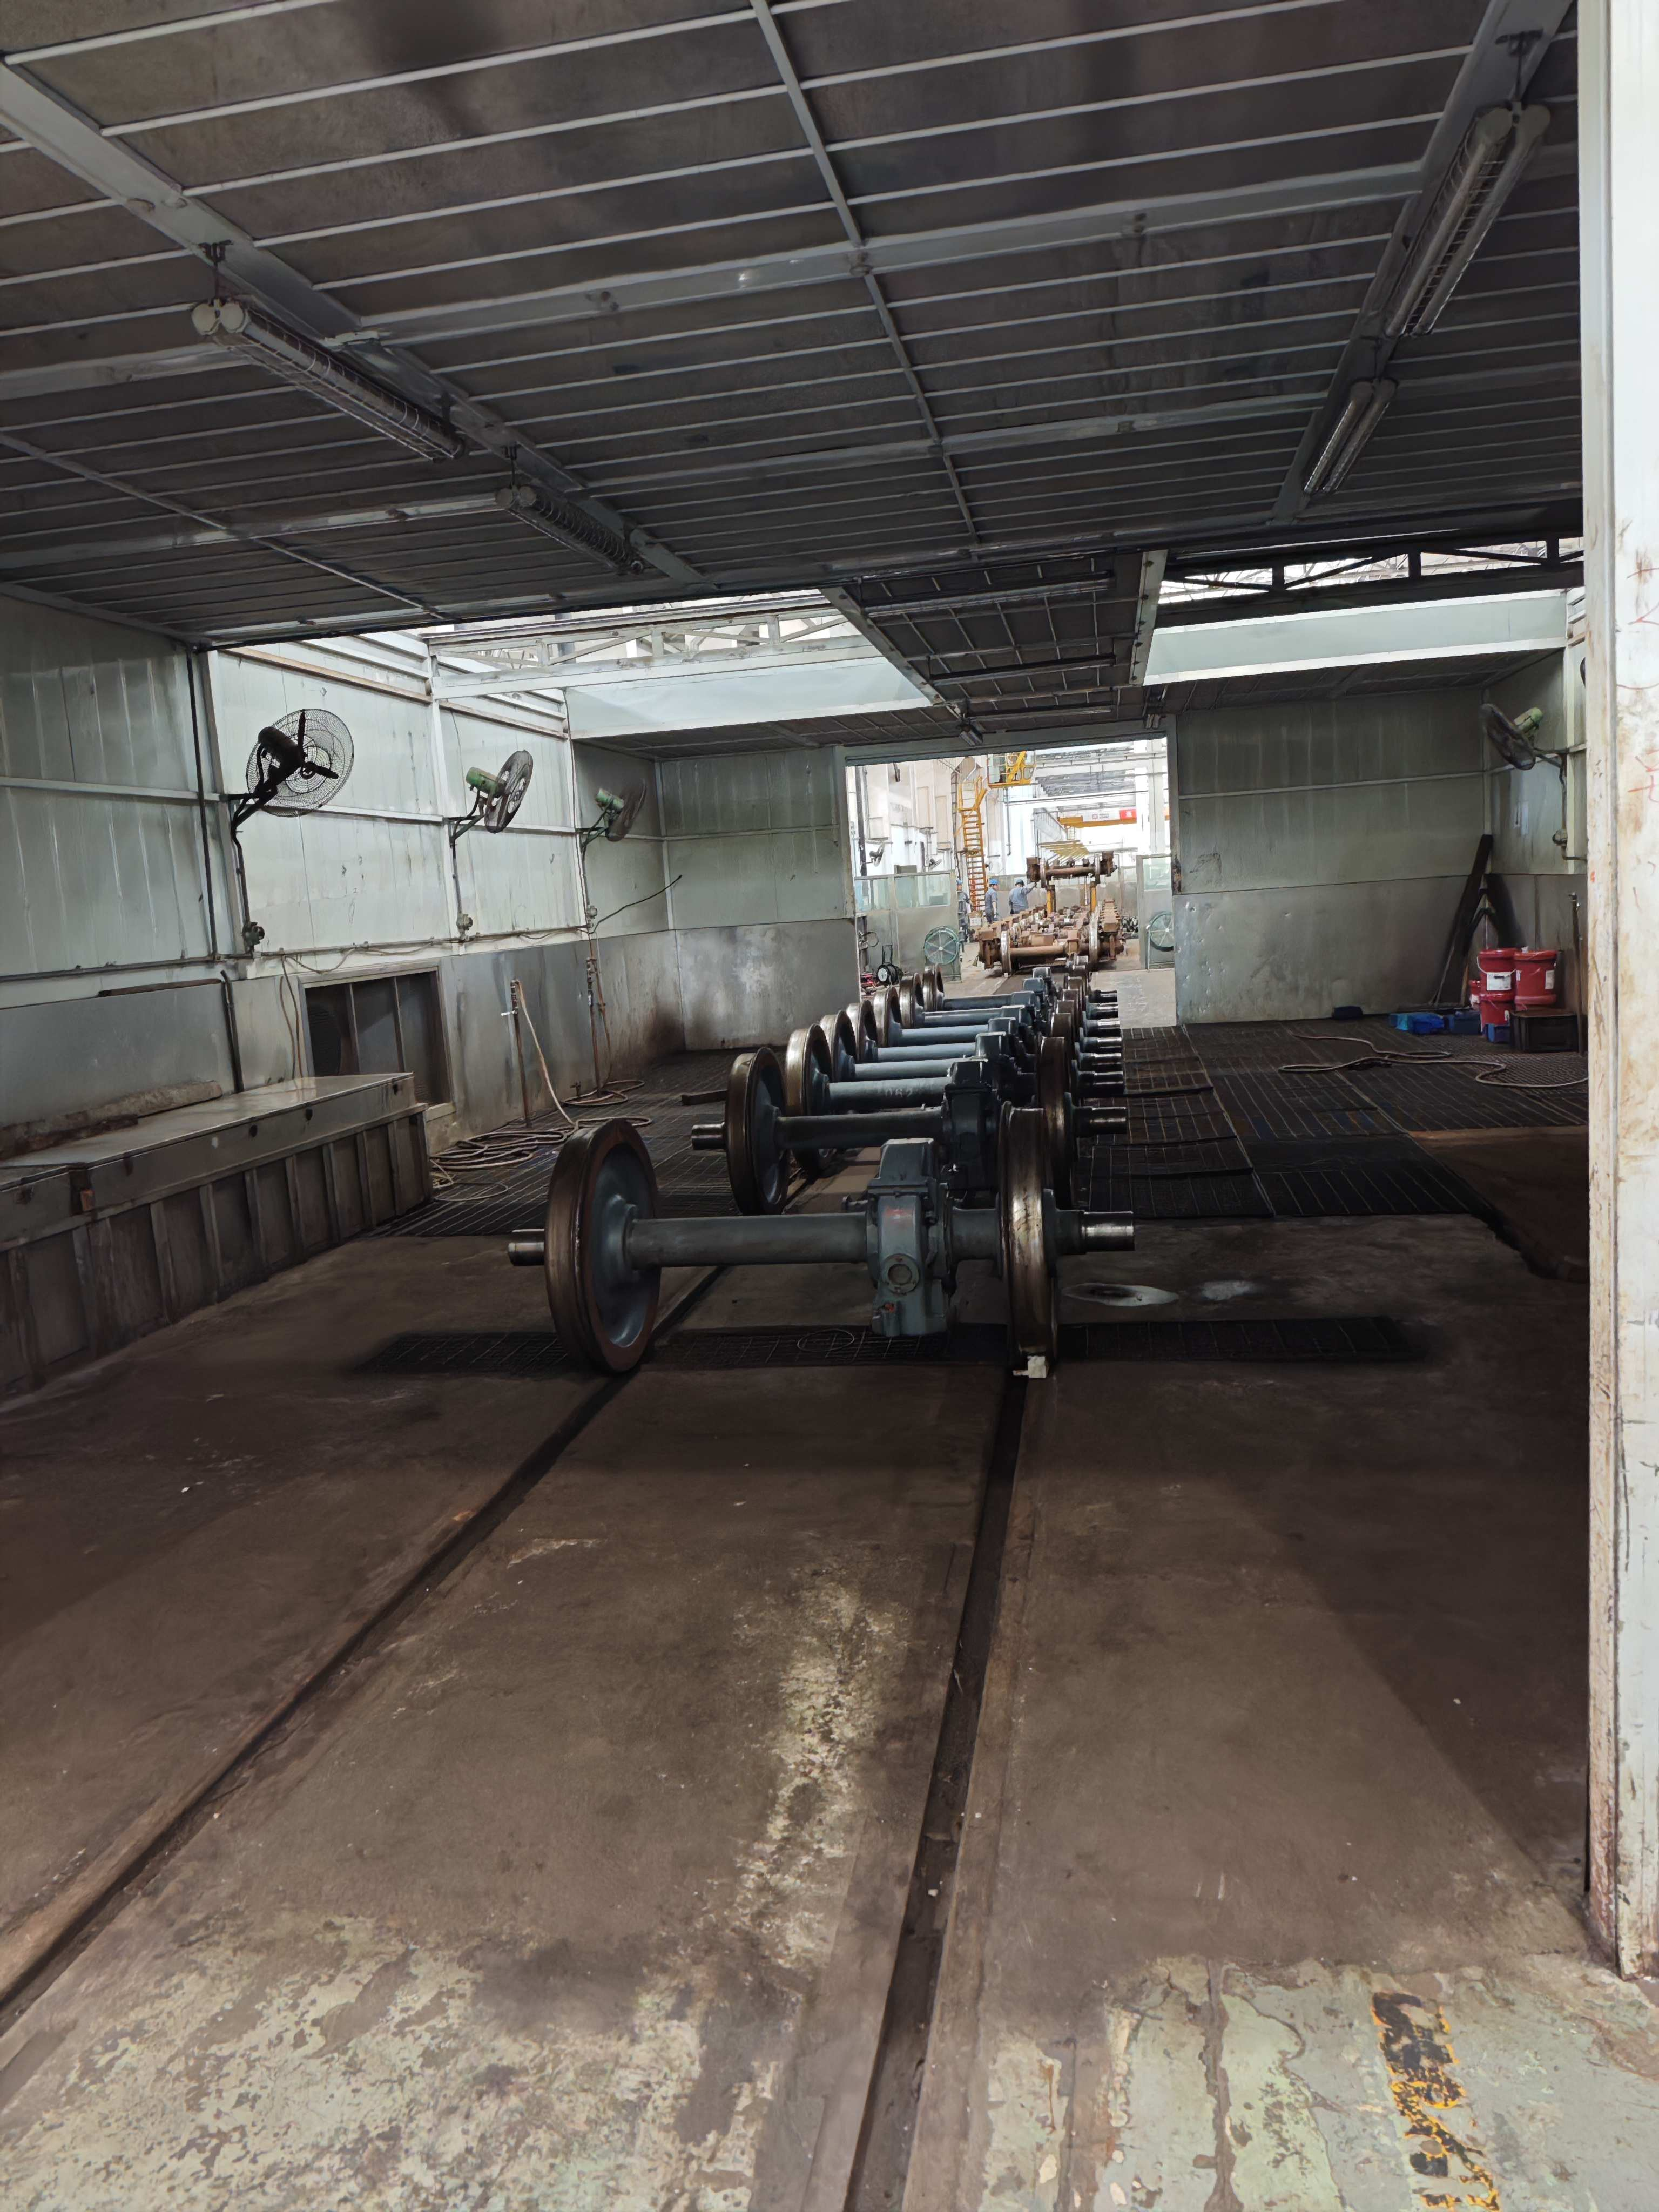
\includegraphics[width=0.45\textwidth]{assets/20260717_035233.jpg}
  \vspace{-2.5mm}
  \caption*{\small{}图13\quad{}一系钢弹簧与轮对}
\end{figure}
\begin{figure}[H]
  \centering
  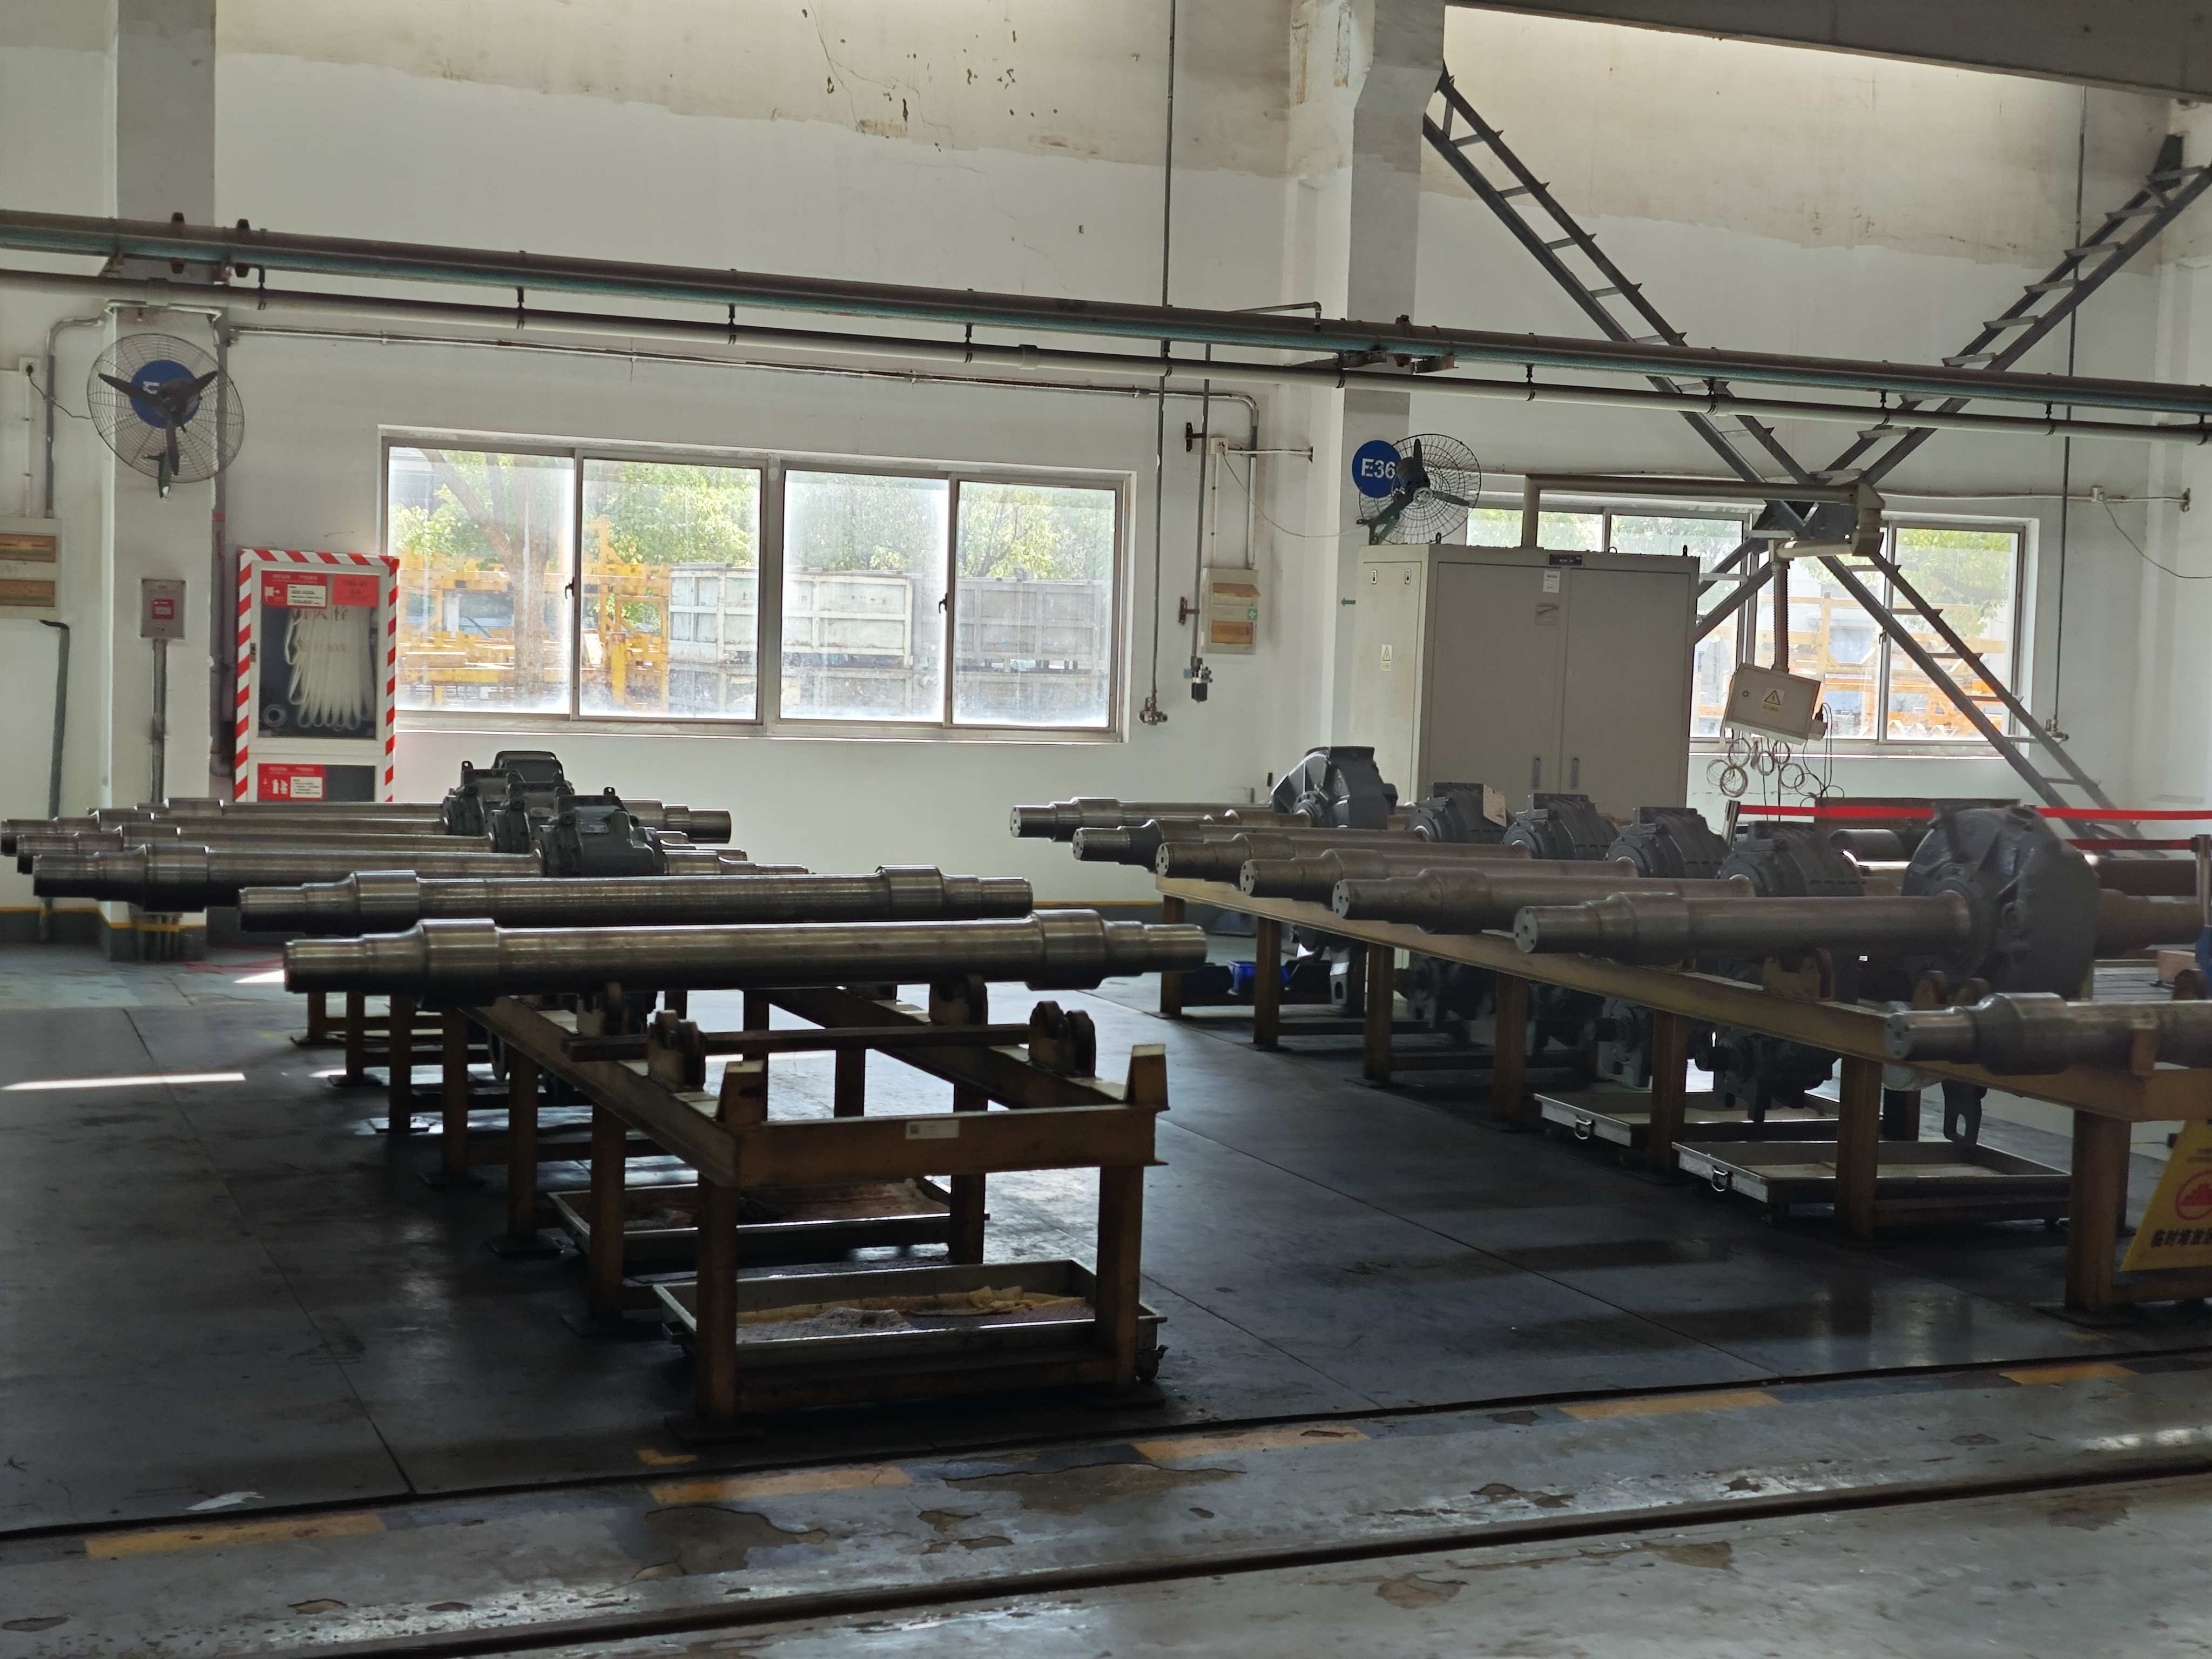
\includegraphics[width=0.8\textwidth]{assets/20260717_040445.jpg}
  \vspace{-2.5mm}
  \caption*{\small{}图14\quad{}已卸去轮的轴}
\end{figure}

\newpage
\journalpage\par{}
图14中，轮对中的轮饼已经被拆卸，剩下的就是轴和齿轮箱。轮饼会进行打磨等处理，以改善其规则度等，而齿轮箱则需要维护，如换油等，轴本身需要进行探伤等检测。结束之后就会再次进行轮对的压装、制动盘的安装等工作，还要进行各类测试与轴箱的安装。图15即为已经安装好轴箱的轮对。\par{}
\begin{figure}[H]
  \centering
  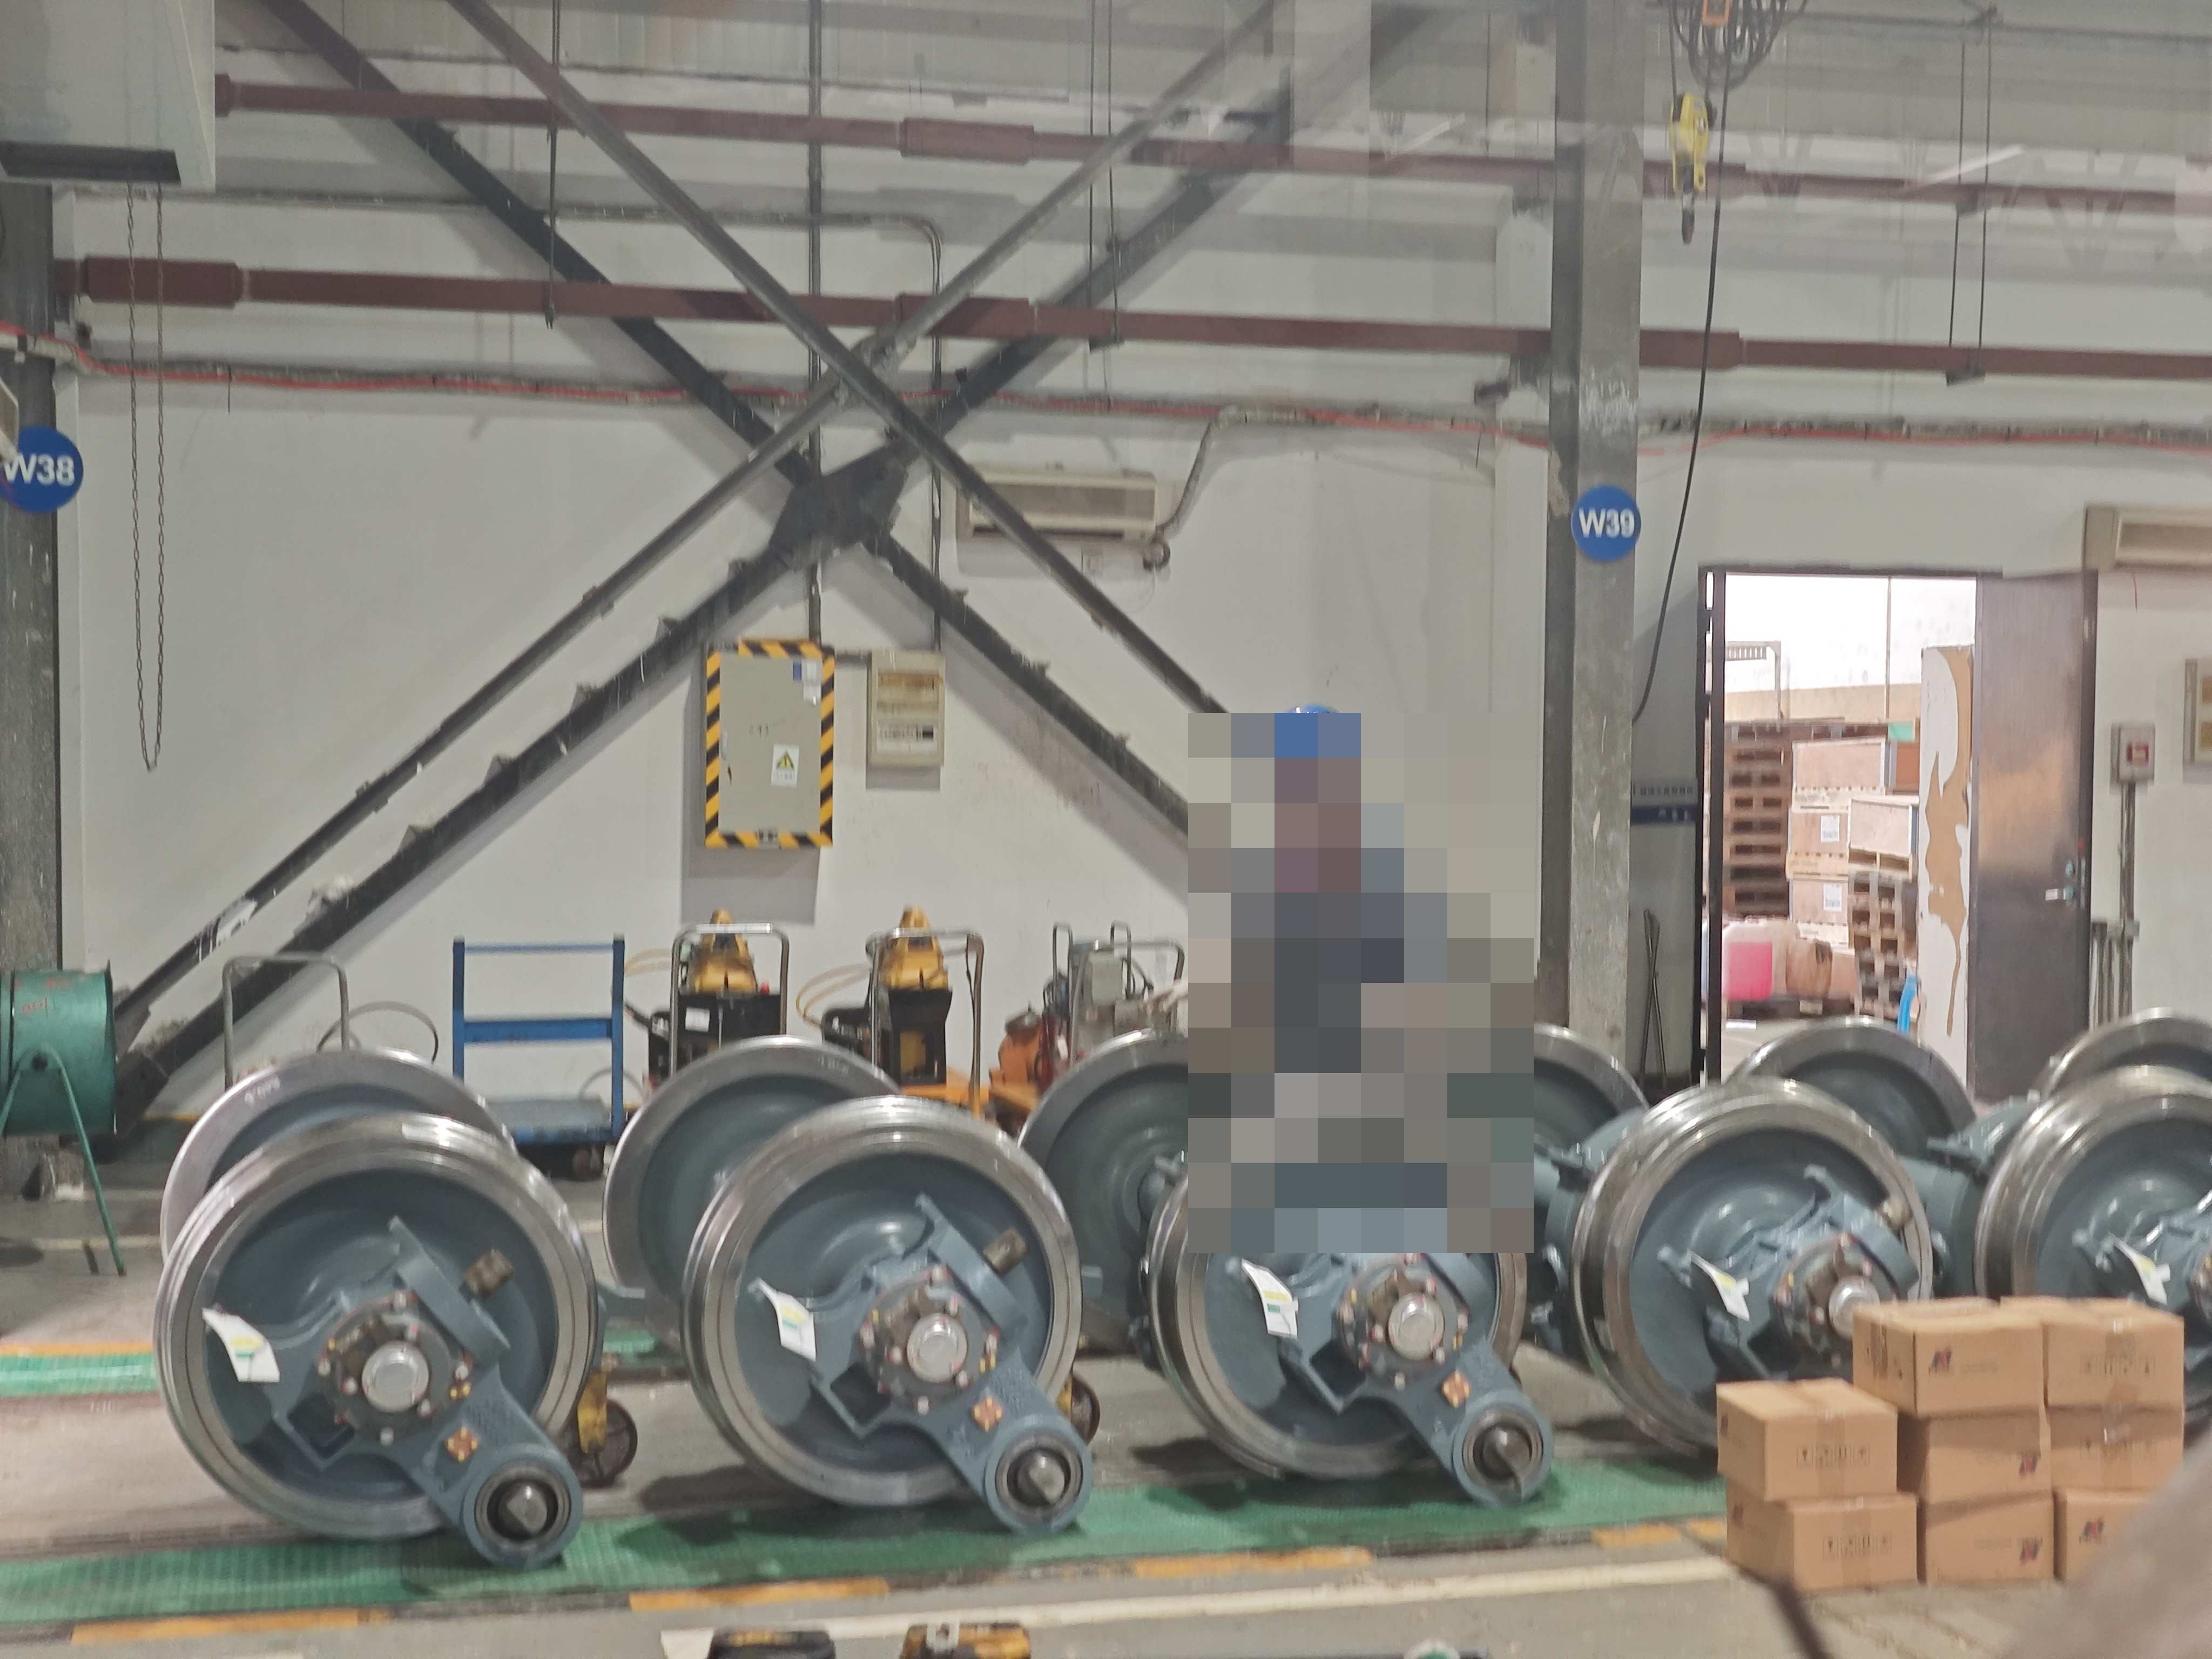
\includegraphics[width=0.8\textwidth]{assets/20260717_040923_worker_mosaic_q55.jpg}
  \vspace{-2.5mm}
  \caption*{\small{}图15\quad{}已安装轴箱的轮对}
  \vspace{-5mm}
\end{figure}
图16为车体、立库与AGV小车。车体没什么可以讲的，而立库和浦镇厂中采用的类似，配合AGV小车可以实现部件的自动化运输。后续的步骤就类似于浦镇厂里的落轮、连挂、静调、动调等，最后就可以再次投入使用了。\par{}
\begin{figure}[H]
  \centering
  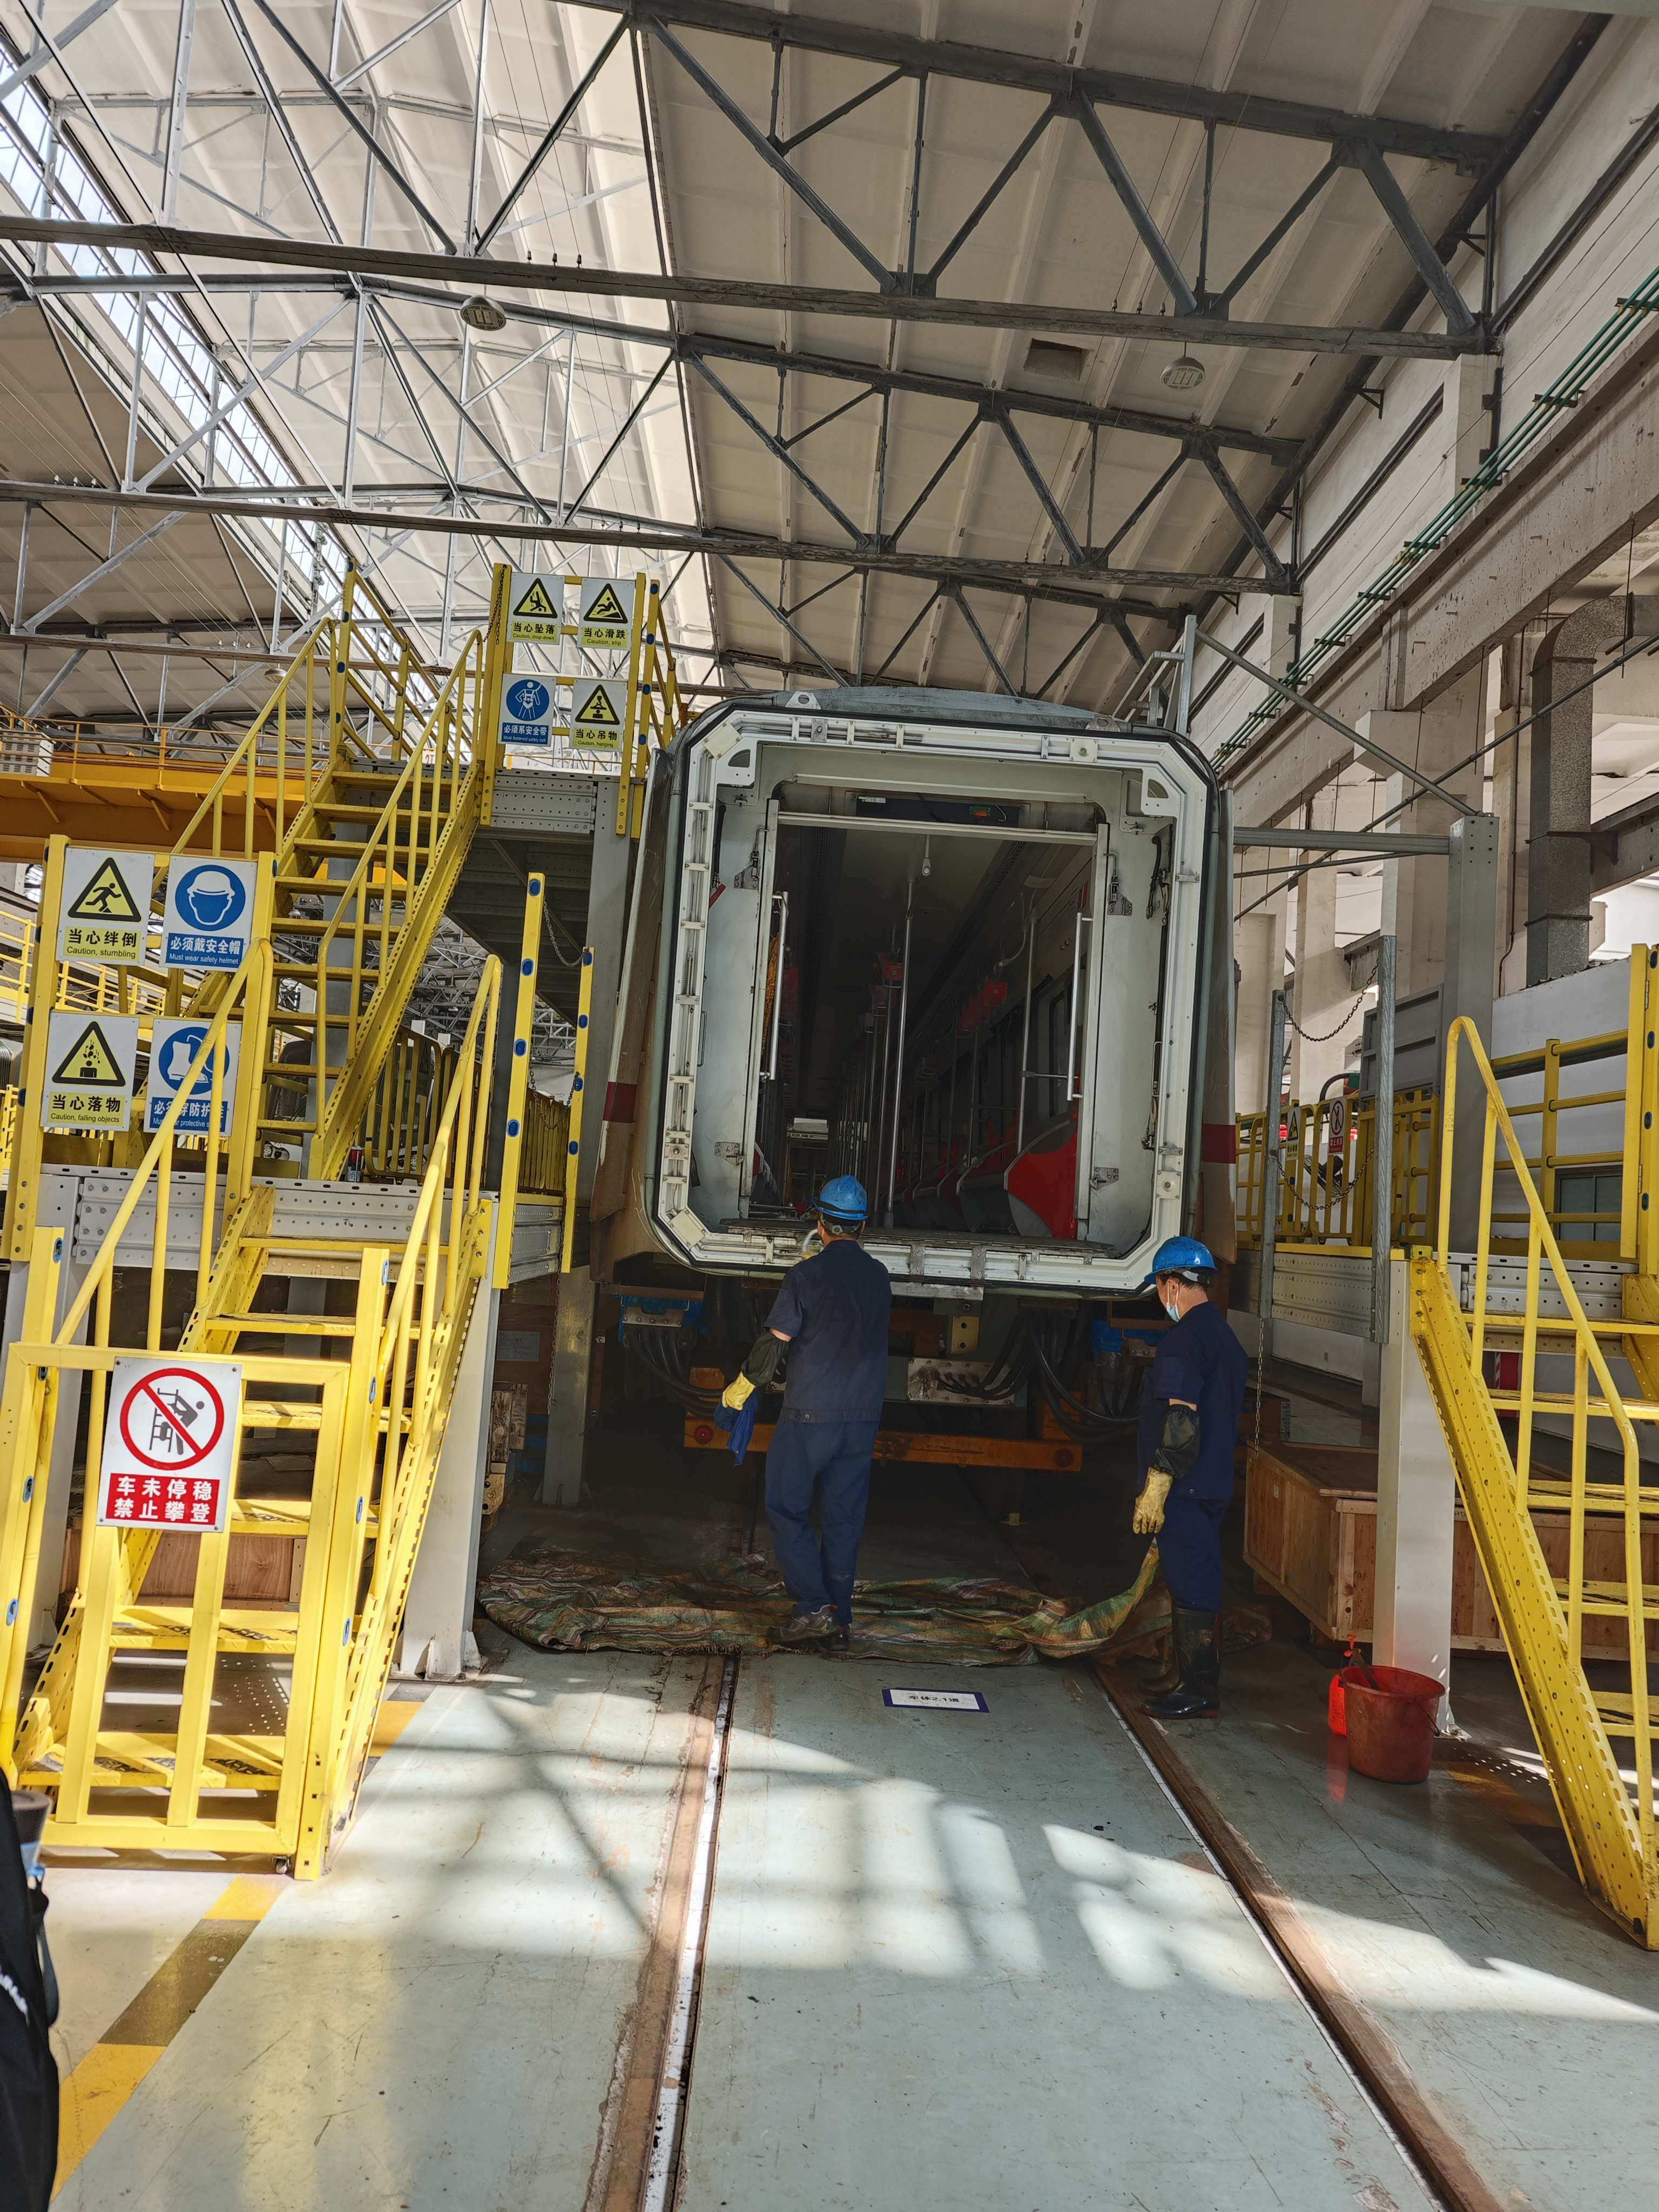
\includegraphics[width=0.35\textwidth]{assets/20260717_041556.jpg}
  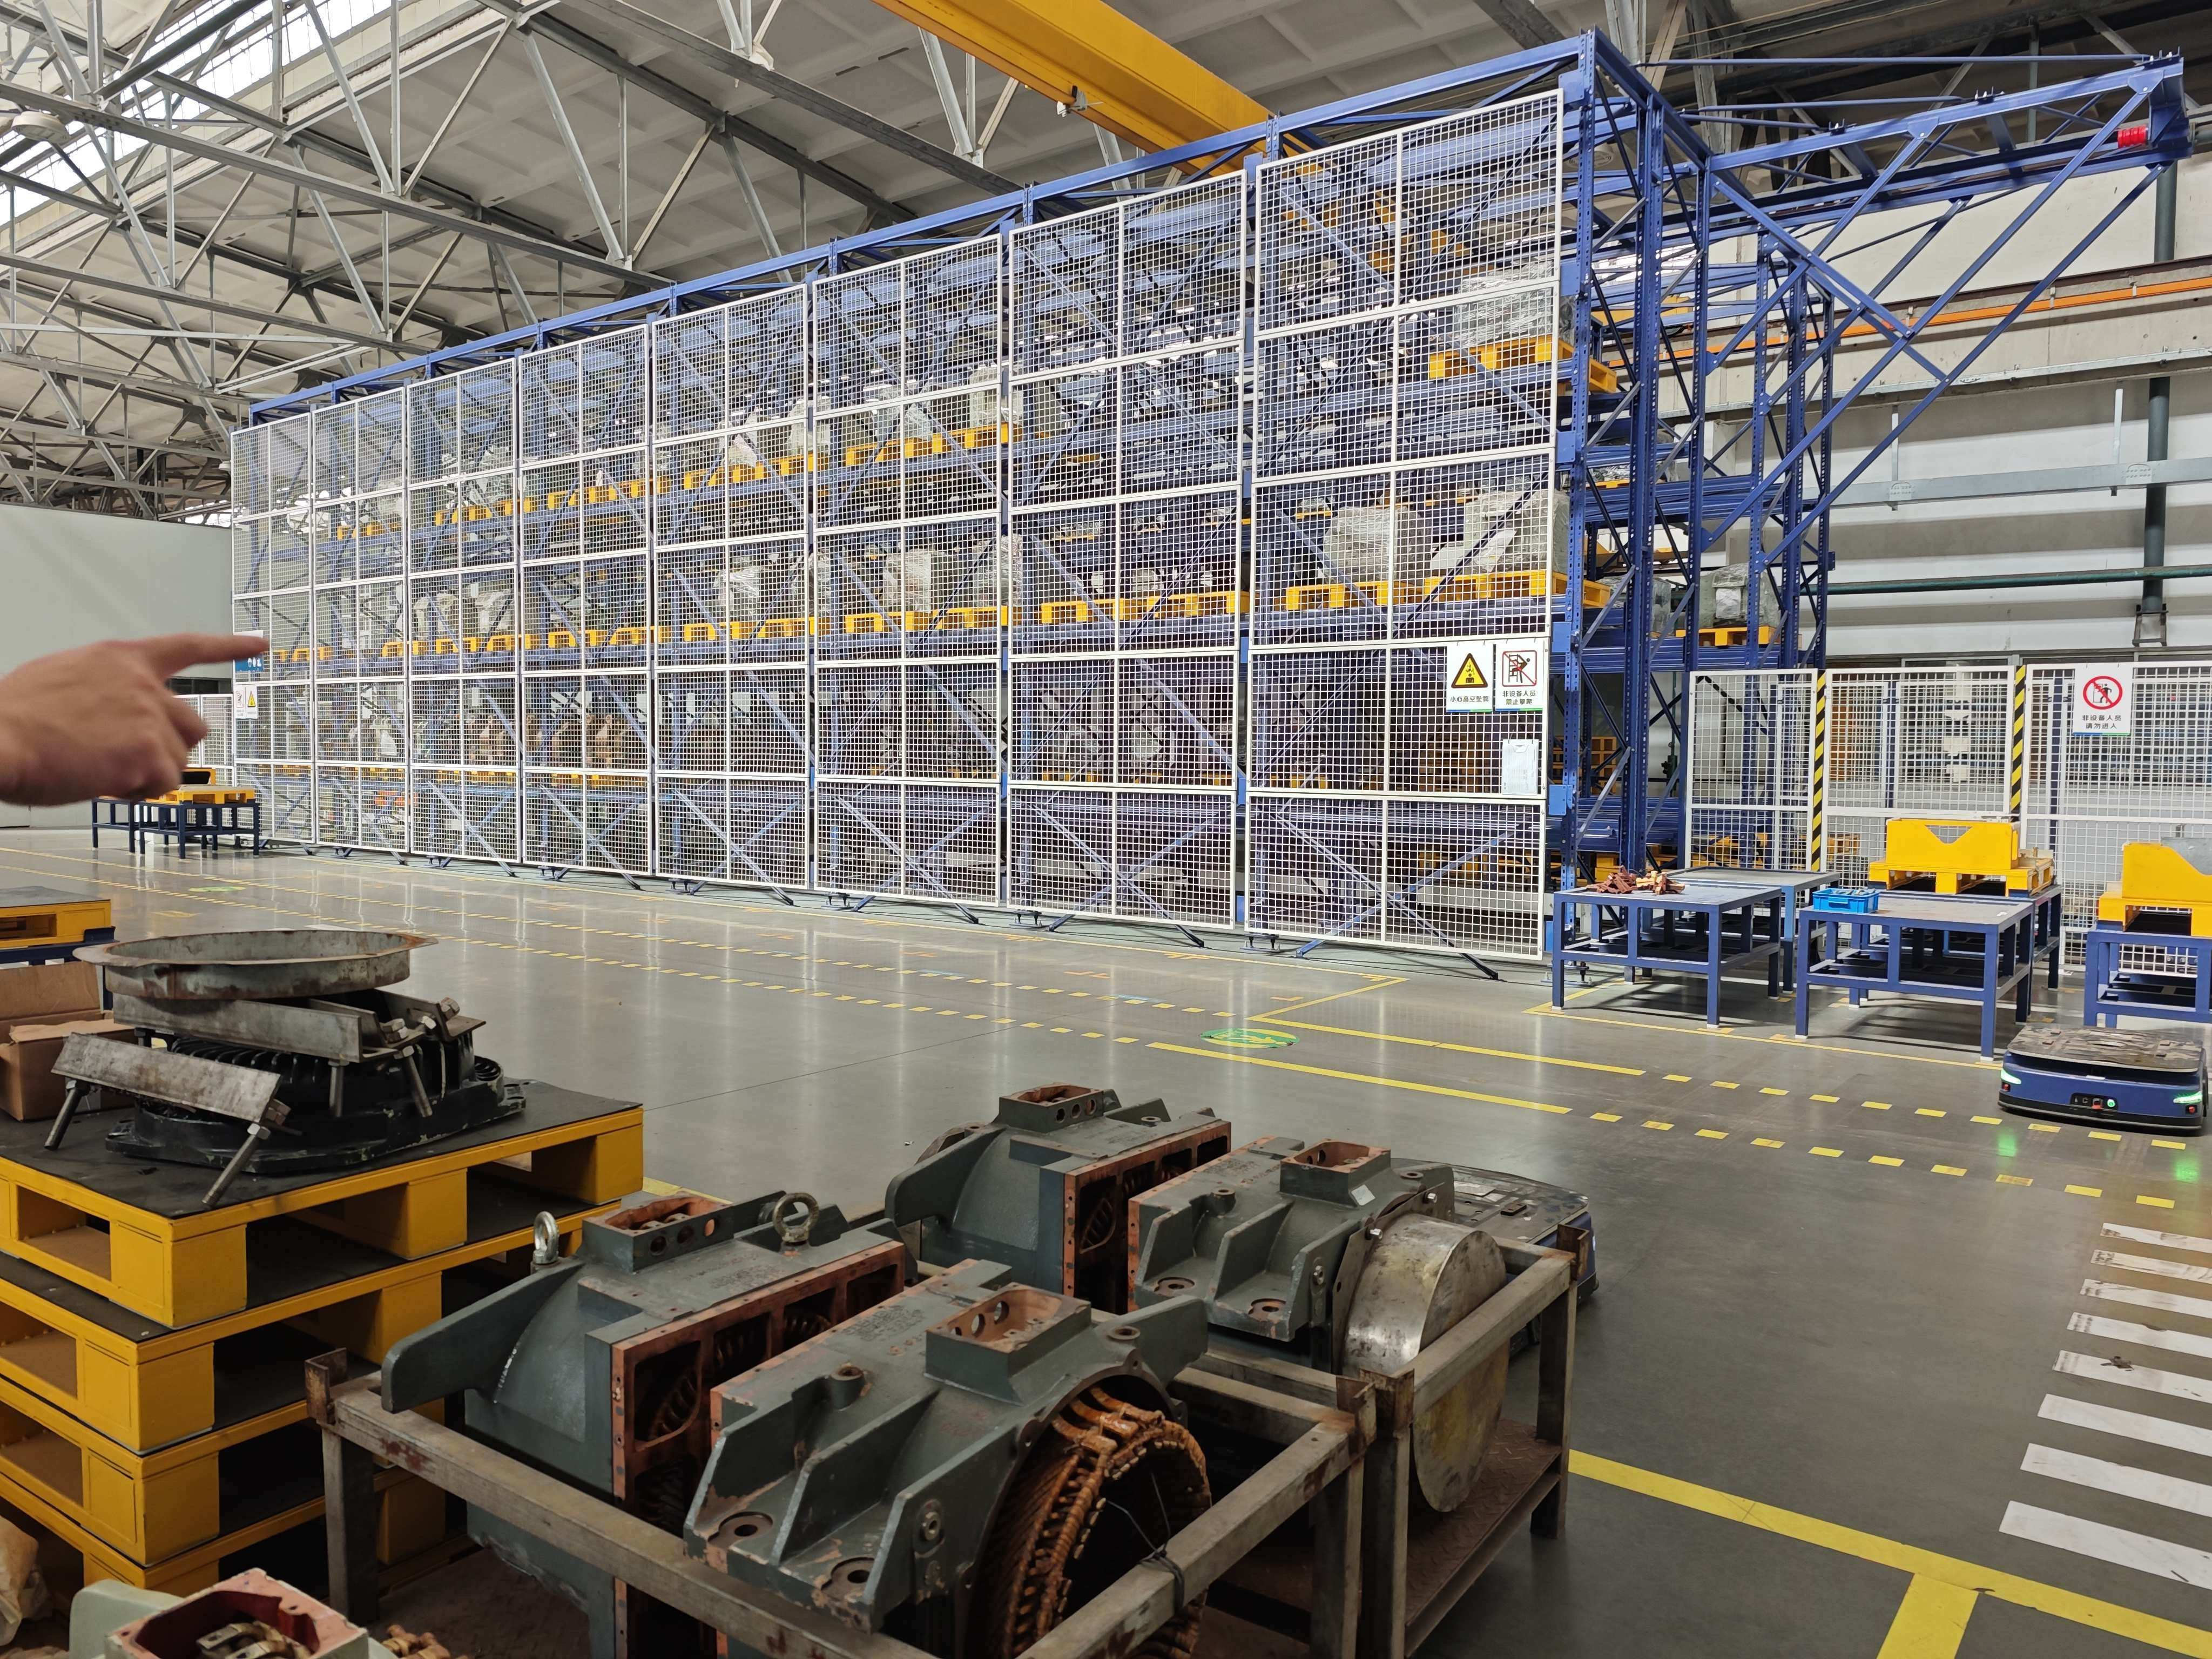
\includegraphics[width=0.63\textwidth]{assets/20260717_042012.jpg}
  \vspace{-2.5mm}
  \caption*{\small{}图16\quad{}车体与立库}
  \vspace{-5mm}
\end{figure}
至此，今日参观到此为止（讲座略），期待明天去梅陇基地。\par{}

\newpage
\journalpage
\vspace{-7.5mm}
\hypertarget{journal-day-0714}{}
\section*{7月14日\quad{}星期二}
\diaryJournalBodyFont\vspace{-3mm}\par{}
今天我们去了梅陇基地，该基地位于上海南站附近，一侧是一号线地上段（上海南站至锦江乐园区间），另一侧是金山铁路。这附近是上海地铁一号线的起点，因此可在图17\sourcecite{2}所示的配线图上看见其里程为“S0+000=0+000”，表示上下行均以此作为起点；此外，类似于赛车场车辆段，梅陇基地也有一个车库加一个维修厂，同时还有与金山铁路相连的国铁联络线。\par{}
\begin{figure}[H]
  \centering
  \vspace{-2.5mm}
  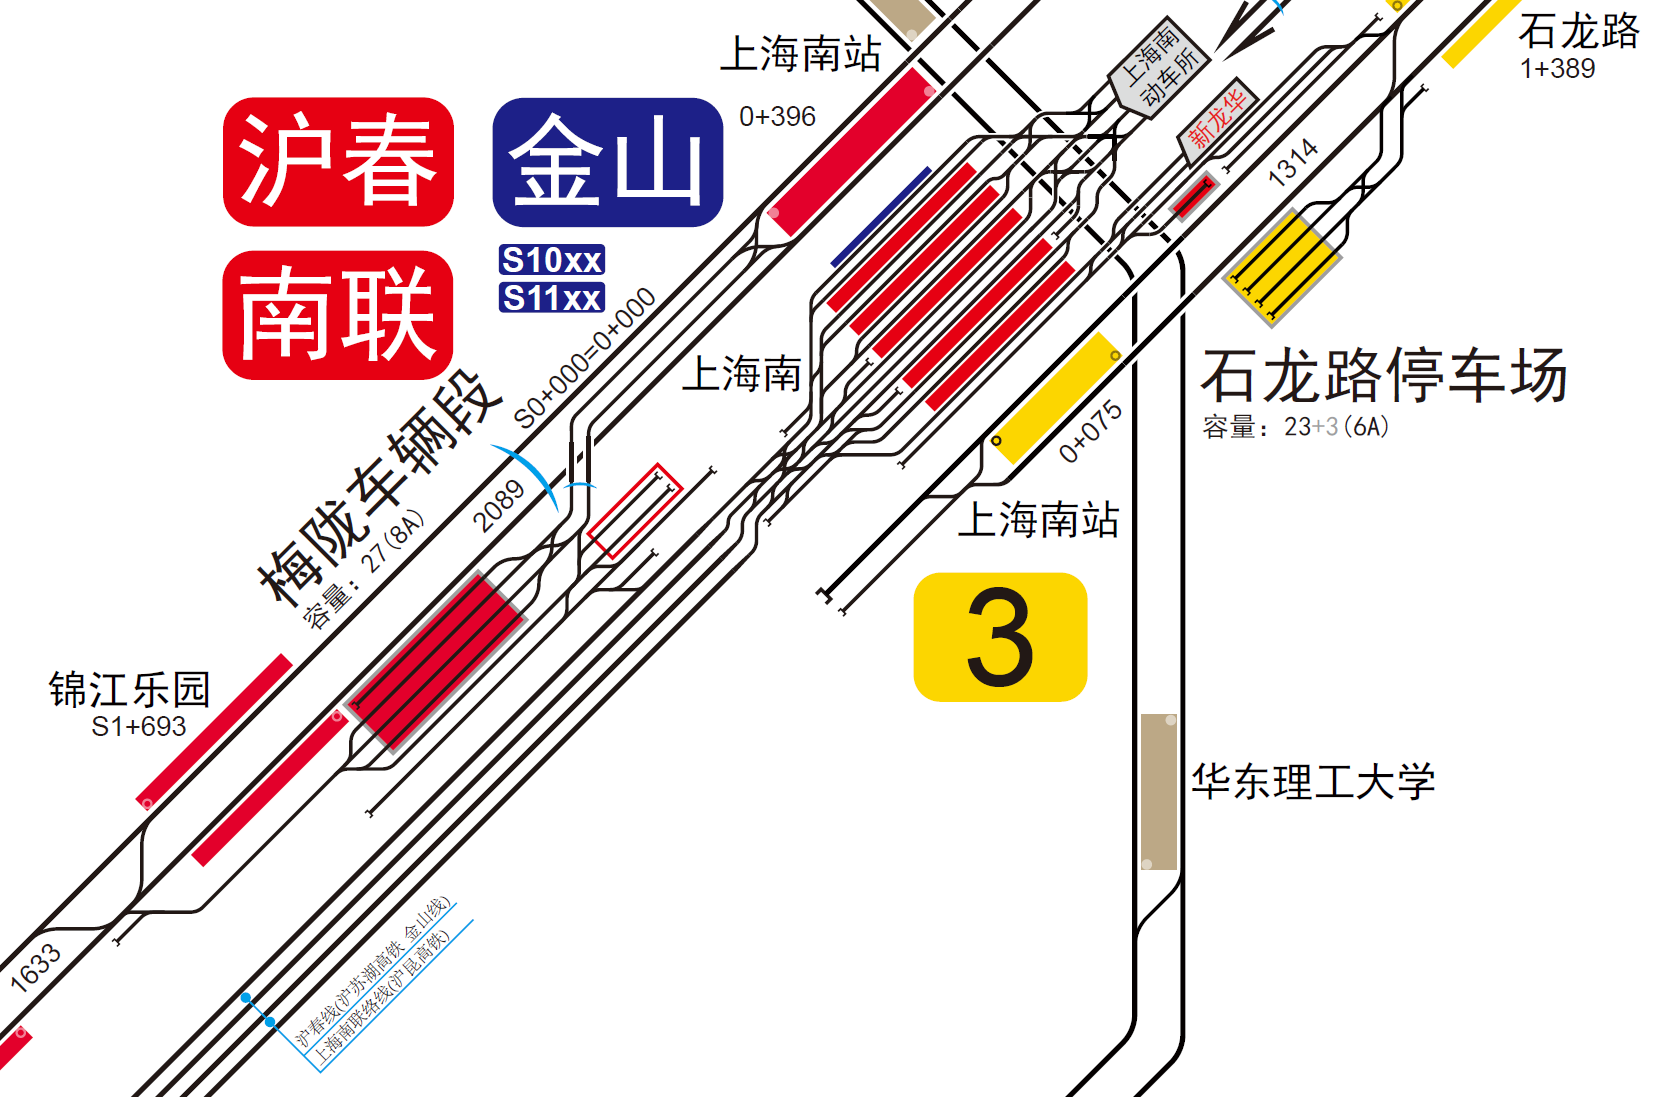
\includegraphics[width=0.6\textwidth]{assets/day7.png}
  \vspace{-2.5mm}
  \caption*{\small{}图17\quad{}梅陇基地位置}
  \vspace{-5mm}
\end{figure}
我们从老沪闵路上的北门进入，左手边就是报告厅和维修厂。我们先去报告厅听了讲座，后去厂内的实验室进行参观。\par{}
\vspace{-5mm}\subsection*{一、 企业介绍}\vspace{-2mm}
首先我们了解了上海地铁维护保障分公司的组织架构（略），接着了解了其人才培养体系。该体系中将人才分为5类对象：新入职员工、青年人才、管理人员、生产人员、拔尖人才，有管理序列、专业技术序列、生产序列3种培养路径，和浦镇厂类似分了11个等级，同时也将员工的发展分为职业导航期、轮岗锻炼期和专业进阶期这3个阶段。\par{}
接着讲了工资、奖金等，还有各类福利，在罗山路还有青年公寓（略）。\par{}
\vspace{-5mm}\subsection*{二、 车辆数字化运维管理中心介绍}\vspace{-2mm}
然后主讲人告知我们不能拍照，接着按下了一个按钮，会议室一侧原本不透光的玻璃幕墙突然变得透明，赫然出现在眼前的就是车辆数字化运维管理中心的大厅，里面的技术人员正在忙碌地工作着。\par{}
面对上海日益发展完善的轨道交通，在车辆业务调整、路网规模扩大、检修模式变化的考量之下，该公司建立了$1+6+33+\mathrm{X}$的指挥布局，即1个车辆数字化运维管理中心、6个车辆数字化运维支持中心、33个车辆控制中心、多个数字化运营协调中心的布局。\par{}

\newpage
\journalpage\par{}
而数字化运维管理中心下又有多个机构：生产调度中心将生产任务构建成时间一定的工作包，使用自动排程系统（APS）拟定生产计划，促进维修模式转型；车场管理中心运用综合管理系统（DCC）实现作业安全预警、车辆实时定位、机器人安全监测等任务；状态监控中心使用车联网（IOR）系统对车辆运行状态进行实时监控；运输支持中心使用应急处置APP和专家系统等支持地铁系统运作；应急指挥中心则开发了应急抢险系统等。\textcolor{gray}{{\bf{}tips: }讲的有点快，还不能拍照，只能简单记一记了，可能有错漏。}\par{}
\vspace{-5mm}\subsection*{三、 实验室参观}\vspace{-2mm}
最后我们去了检验检测部的实验室进行参观。该实验室在2020年开始筹备建造、2023年正式成立，初衷是智能运维需要大量数据支持，因此需要通过实验室来获取大量的现场使用的检测数据。其业务包括来样检测、抽样检测、验车检测等，来样检测是指列车发生故障时回库换下的故障设备运送到实验室进行分析，抽样检测是指对修缮完毕的列车的关键部件进行抽样检查，验车检测是登上列车进行现场检测。\par{}
\vspace{-5mm}\subsubsection*{3.1\quad{}齿轮箱润滑油实验室}\vspace{-2mm}
我们参观的第一个实验室是齿轮箱润滑油实验室（具体叫什么没记）。齿轮箱润滑油在齿轮箱润滑、缓解齿轮箱磨损上有重要作用，一般需要一年更换一次；然而，一般的4M2T编组就有$4 \times 2 \times 2 = 16$个齿轮箱（4节动车的2个转向架上分别有2个轮对都有齿轮箱），上海地铁全路几千辆车，每年每车都换油，消耗量巨大，不利于降本增效。因此可以对车辆换下的润滑油进行检测，如果超过1年外观仍然清澈，那么需要进一步检测其他参数，确定是否可复用，避免浪费。\par{}
主要检测内容就是先取油，搅拌均匀后对水含量、黏度、Cu与Fe等金属离子含量进行检测，会使用到光谱仪。\par{}
\vspace{-5mm}\subsubsection*{3.2\quad{}控制板卡实验室}\vspace{-2mm}
该实验室有3个试验台。\par{}
第1个试验台是门控器试验台。门控器主要由$\mathrm{PLC}$+电源+电机驱动器组成，该试验台专门用于检测车门控制板卡的信号收发、输出功率、电压波形等。\par{}
第2个试验台是继电器试验台。由课内知识可得，继电器有这种机械式的，也有大功率开关管形成的固态继电器，这种机械式的继电器由于开关频繁，关键部件可能会出现机械卡死、热失效等故障，因此需要进行试验。\par{}
第3个试验台是报站系统试验台。虽然报站与显示不影响列车运行本身，但是报站错误会导致乘客投诉，降低运营效率，因此也需要进行检测。\par{}

\newpage
\journalpage\par{}
\vspace{-5mm}\subsubsection*{3.3\quad{}车辆低压电气实验室}\vspace{-2mm}
该实验室有2个试验台。\par{}
第1个试验台是速度传感器试验台。一般速度传感器采用霍尔式等，根据记录的双脉冲来推算齿轮的转速，进而得知车速；双脉冲比单脉冲的优势就在于其可以同时反映速度大小和方向。速度传感器的准确度主要受其工作环境影响，振动、温度、齿轮箱漏油等可能会使得漏掉脉冲、速度记录出错，因此需要进行检测。\par{}
第2个试验台是电气元件综合试验台。该试验台通过模拟振动和温度来对电气元件进行测试。\par{}
\vspace{-5mm}\subsubsection*{3.4\quad{}其他实验室}\vspace{-2mm}
后续我们还参观了全相检测实验室、车辆高压电气实验室等，其中前者主要对走行部进行检测，后者主要对牵引逆变器、受电弓等进行检测。但由于各种原因，当时记录的字迹难以辨认，因此这里略去。\par{}

\newpage
\journalpage
\vspace{-7.5mm}
\hypertarget{journal-day-0715}{}
\section*{7月15日\quad{}星期三}
\diaryJournalBodyFont\vspace{-3mm}\par{}
今天我们去了位于闵行开发区的上海阿尔斯通（中车长客）公司，位置大致如图18\sourcecite{2}，在闵行开发区站西侧。\par{}
\begin{figure}[H]
  \centering
  \vspace{-2.5mm}
  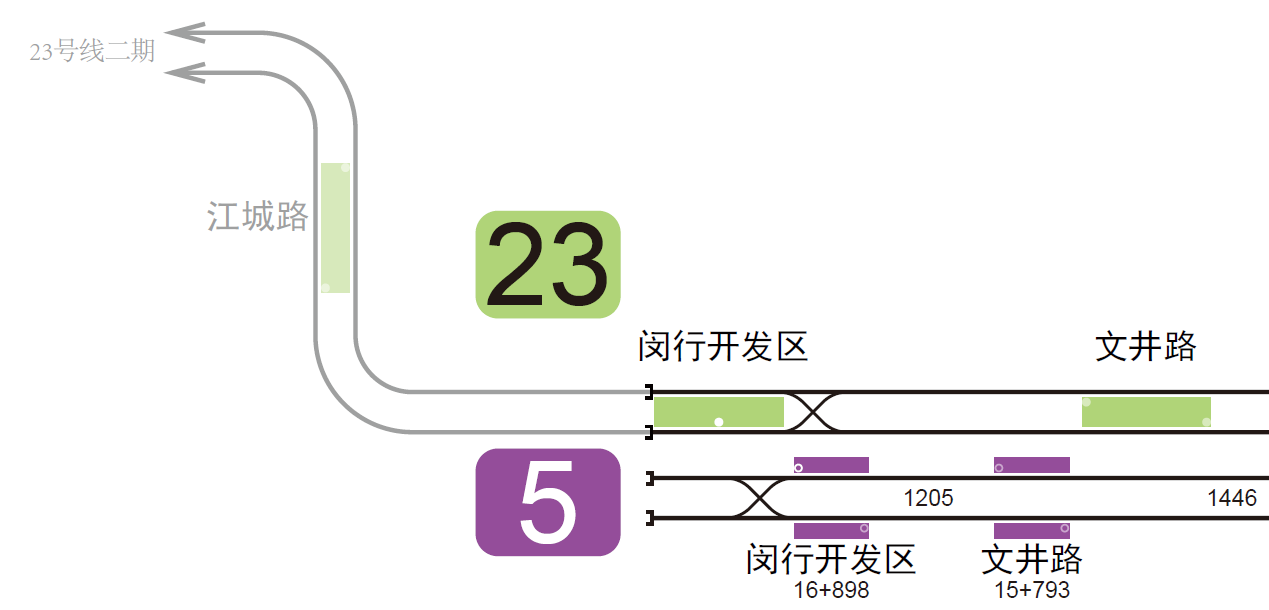
\includegraphics[width=0.6\textwidth]{assets/day8.png}
  \vspace{-2.5mm}
  \caption*{\small{}图18\quad{}上海阿尔斯通（中车长客）公司位置}
  \vspace{-5mm}
\end{figure}
由于今天天气较热，所有项目均为室内讲座，下面是对讲座内容的记录。\par{}
\vspace{-5mm}\subsection*{一、 公司介绍}\vspace{-2mm}
该公司全称上海轨道交通设备发展有限公司，由中车长客、上海电气等共同持股，融合阿尔斯通等品牌、资源、技术优势，下属上海中车长客交通设备有限公司（原SATCO）、上海阿尔斯通交通电气有限公司（SATEE）、工程公司等子公司、联营公司或独立分公司。\par{}
原SATCO具有从车辆设计，到组装、涂装、总装、调试、质保、维修的一系列完整产业链，参与了多种上海地铁车型的设计；而SATEE则负责生产牵引系统设备、辅助变流器及其相关电气设备，是国内具有投标资质的定点生产牵引传动与控制系统的企业，先前在浦镇公司看到的上海21号线列车的车下电气设备就是该公司的产品；而工程公司则负责设计制造安装屏蔽门、安全门等产品，还具备供电、车站、车辆段等设备集成与施工安装的能力等。\par{}
\vspace{-5mm}\subsection*{二、 上海工程技术研究中心介绍}\vspace{-2mm}
该中心的功能定位为：补齐公司技术短板、引领特色技术领域、支撑区域化经营、输出技术及服务。其下属4个部门，分别为综合管理部、核心技术研发部、系统集成研发部、城铁车辆研发部。其主要车辆产品有地铁车辆、市域车、有轨电车、车辆设备等，参与了上海某些地铁线路的车辆设计、金华-义乌-东阳市域车设计、嘉兴有轨电车设计等设计任务，也在上海地铁完成了多种车辆的升级改造任务，同时还有一些售后等服务。\par{}
\vspace{-5mm}\subsection*{三、 新线路及其车辆设计概述}\vspace{-2mm}
将来，除了机场联络线，上海还会有3条市域线：南汇线、青浦示范区线、嘉闵线。车辆均采用市域C型车，注意市域车的规格同地铁有所区别，市域A\par{}

\newpage
\journalpage\par\noindent
型车尺寸大致等于地铁A型车，B型车也类似，但是C型车是基于高铁动车组，如“复兴号”，进行降速降配、城铁化而来，可以4节编组、8节编组或4+4重联编组运行（两车连挂需要同步信号等设备才算重联，否则可能是救援）。\par{}
接着还讲了规划或建设中的上海“新五线”，即$19\sim23$号线的地铁列车设计方案，包括造型、配色等。这五条线都是无人驾驶车辆，但是仍然配有“司机”和“司机室”，只不过“司机室”没有占满整个车头宽度，车头处空余部分还留出了朝前开的逃生门。至于为什么还要配备“司机”，这是因为机破时仍然需要专业人员进行排障、指引乘客等操作。\par{}
今日的学习就到这里，明天去上海动车段，也是最后一天，加油！\par{}

\newpage
\journalpage
\vspace{-7.5mm}
\hypertarget{journal-day-0716}{}
\section*{7月16日\quad{}星期四}
\diaryJournalBodyFont\vspace{-3mm}\par{}
今天我们去了上海动车段动车组高级修场，其为全路率先建成的四个高修场地之一，位于南翔编组站南侧，通过西走行线与上海虹桥动车所、上海虹桥站连接，通过东走行线与南翔动车所、上海西站（原真如站）、上海站连接，如图19\sourcecite{2}所示。\par{}
\begin{figure}[H]
  \centering
  \vspace{-2.5mm}
  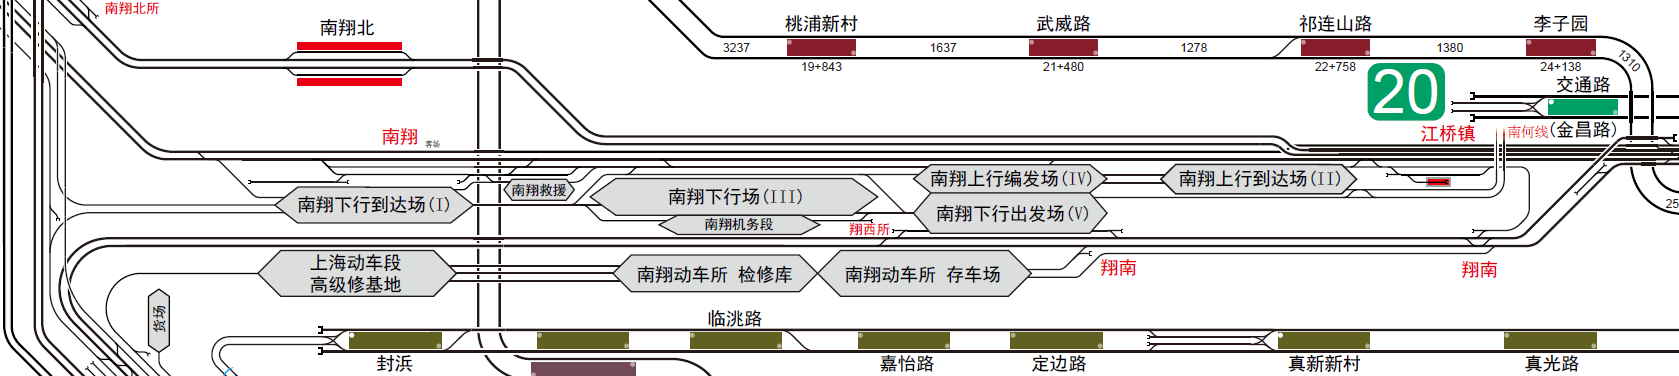
\includegraphics[width=0.98\textwidth]{assets/day9.png}
  \vspace{-2.5mm}
  \caption*{\small{}图19\quad{}上海动车段动车组高级修场位置}
  \vspace{-5mm}
\end{figure}
而其场内布局如图20所示：\par{}
\begin{figure}[H]
  \centering
  \vspace{-2.5mm}
  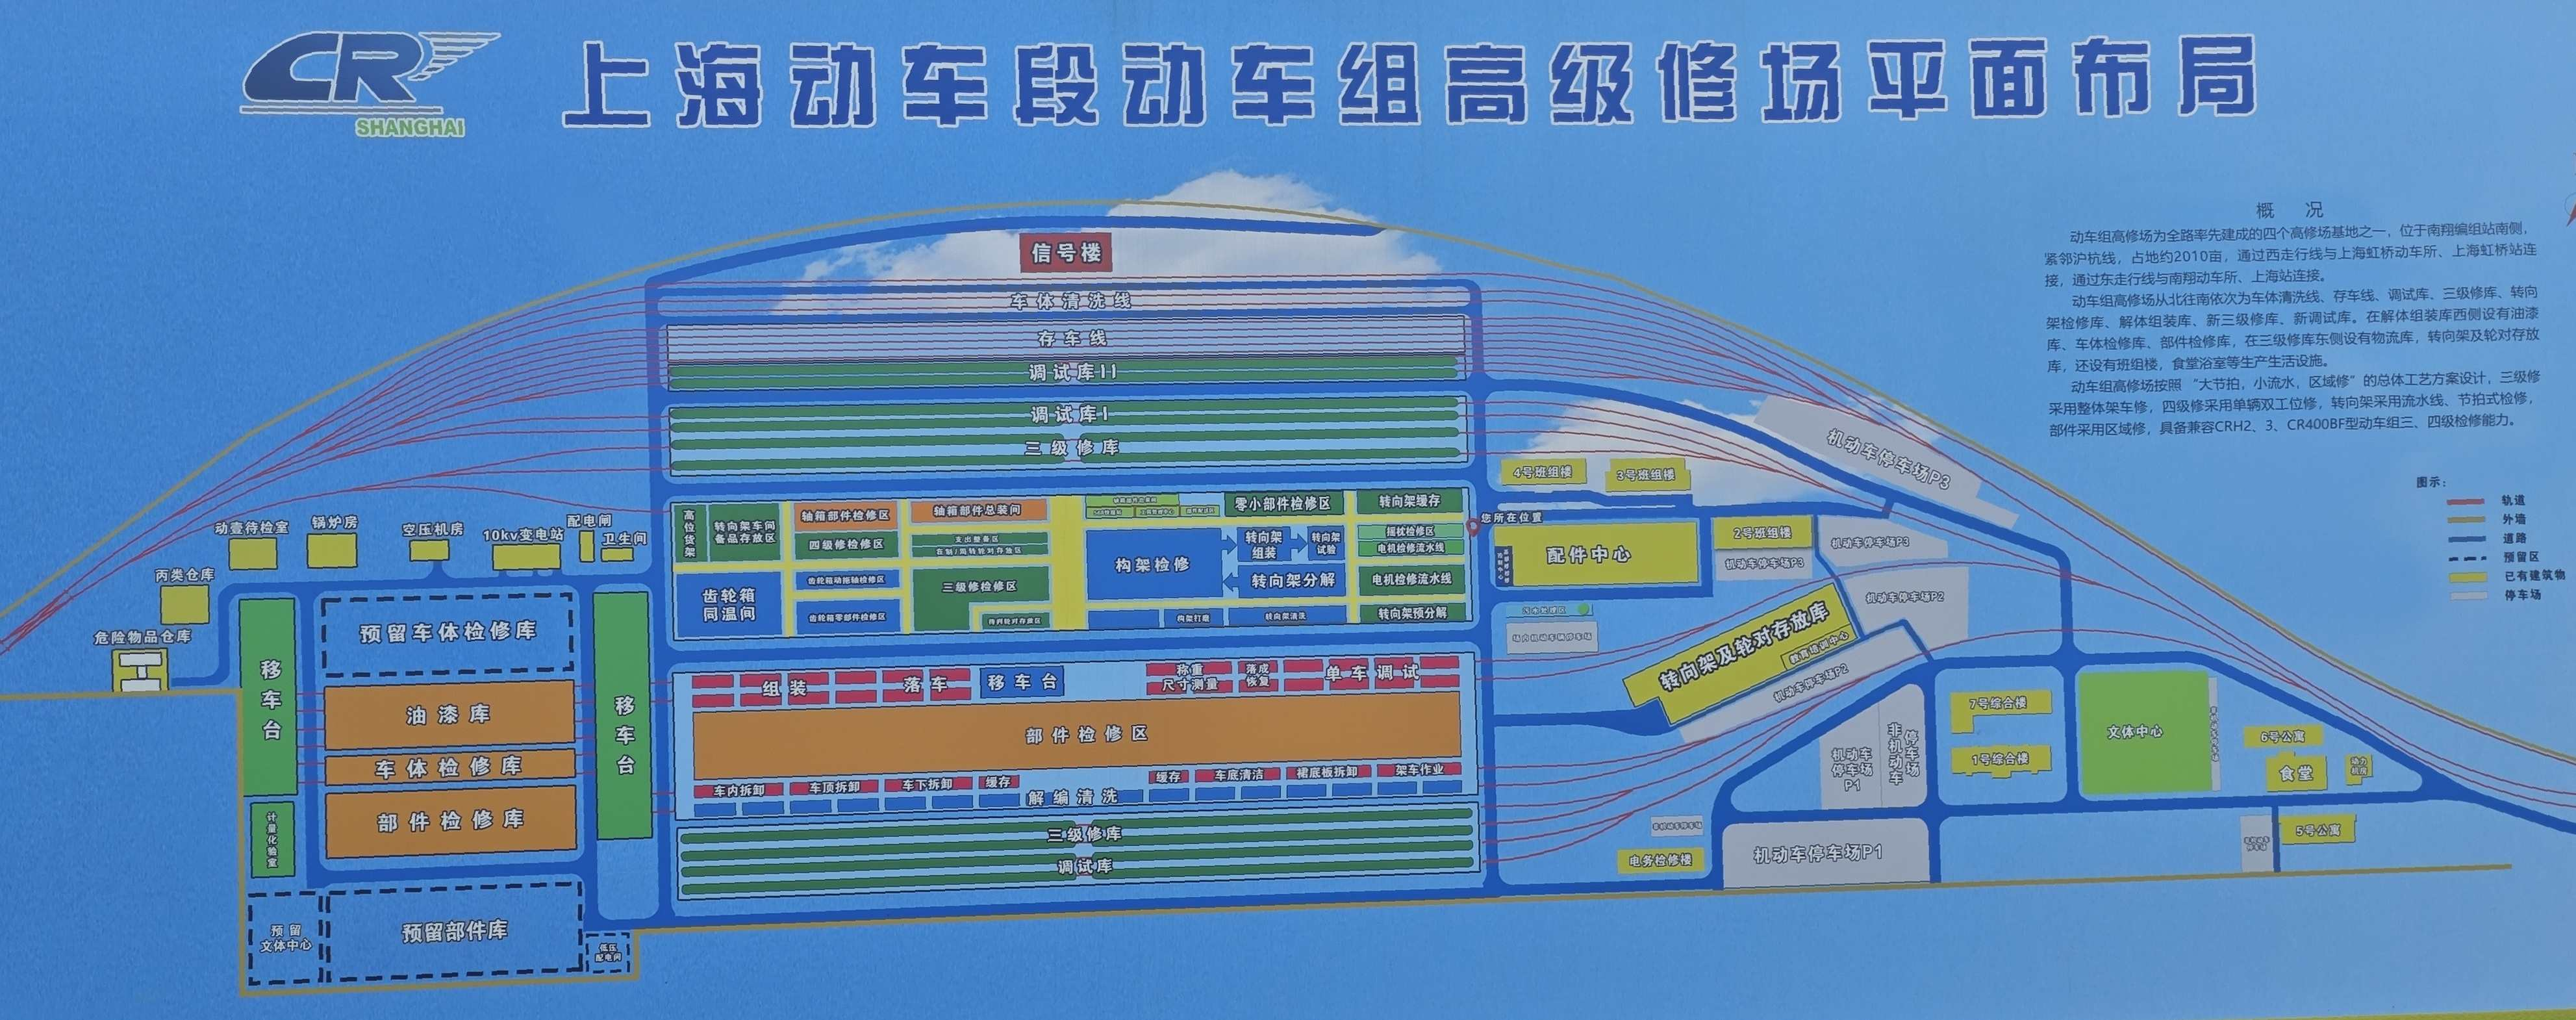
\includegraphics[width=0.98\textwidth]{assets/20260718_211523.jpg}
  \vspace{-2.5mm}
  \caption*{\small{}图20\quad{}上海动车段动车组高级修场内部布局图}
  \vspace{-5mm}
\end{figure}
今天我们要参观的就是一号库（图中调试库I + 三级检修库）、三号库（即图中部件检修区/解编修库）、高级修检修控制中心（MCC，即图中配件中心）。\par{}
\vspace{-5mm}\subsection*{一、 一号库 - 三级检修库}\vspace{-2mm}
这些个检修库不同于动车运用所，前者，也就是文中所在的位置，是指列车定期的检查与修理场所，一般修理较为完全与彻底；后者是每天车次运行完结，列车返回的地方，只进行常规检查，一般以夜班为主，尤其是春运时非常忙碌。\par{}
进入库内，其D12股道上停了一列车，车型车号为CRH380BL-3545，中车唐山制造，配属上局南京段。\par{}
该车这几天已经基本完成三级修主要内容，即接车预检、预检后调车、解编、架车、车体检修、转向架检修、落车、尺寸测量与称重，正在调试库中进行落成恢复、单车调试、编组的工序，后续还将进行静态调试、动态调试、动调后检查、淋雨试验等，是典型的三级高级修流程\sourcecite{3}。\par{}

\newpage
\journalpage\par\noindent
\begin{figure}[H]
  \centering
  \vspace{-2.5mm}
  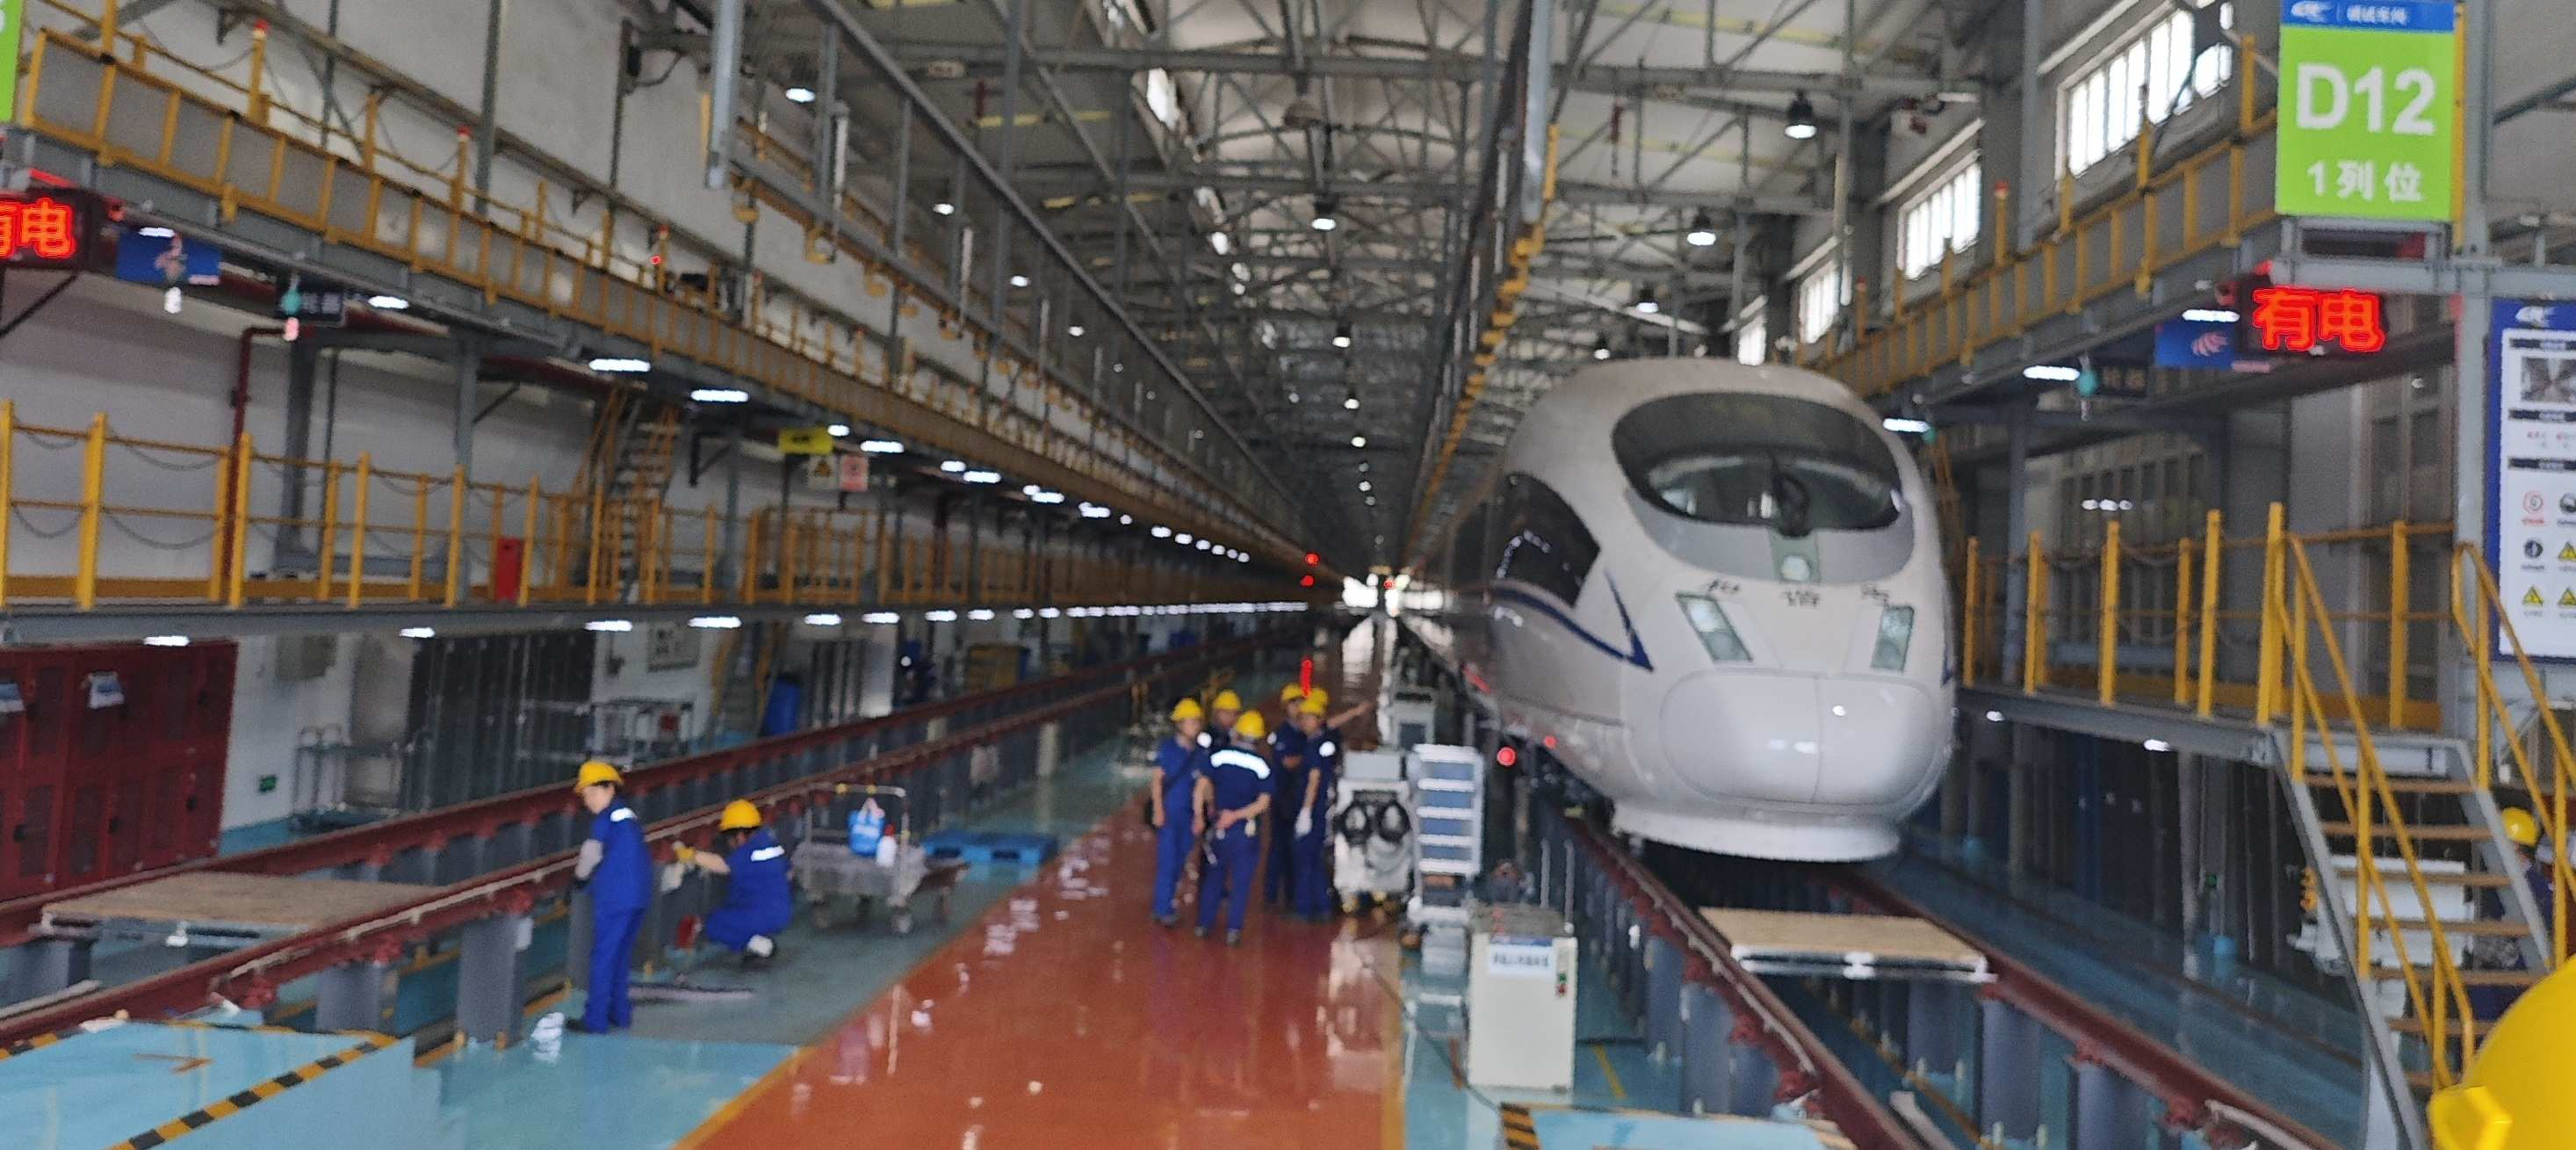
\includegraphics[width=0.8\textwidth]{assets/20260718_212836.jpg}
  \vspace{-2.5mm}
  \caption*{\small{}图21\quad{}正在检修的CRH380BL-3545列车}
  \vspace{-5mm}
\end{figure}
上方接触网显示“有电”，说明此时正在进行通电试验，在通电或断电的过程中，都要求附近人员远离车辆与接触网，在断电后还要人为在触网上悬挂接地线，车体旁的走廊/高站也分为好几层，第三层的平台只有相关资质的人员才能入内。\par{}
图22（左）所示的设备就是计算轴重的设备，位于检修库出入口处，主要是测量列车左右重量是否平衡，一般要求偏差不超过$4\%$或$8\%$；图22（中）所示的设备是用于转移车辆转向架的落坑式（没听清，应该叫这个名字）平台，可以通过下沉的方式将转向架从下方转移；图22（右）的设备是用于防止溜车的铁鞋。大部分设备都是中车青岛四方公司制造的。\par{}
\begin{figure}[H]
  \centering
  \vspace{-2.5mm}
  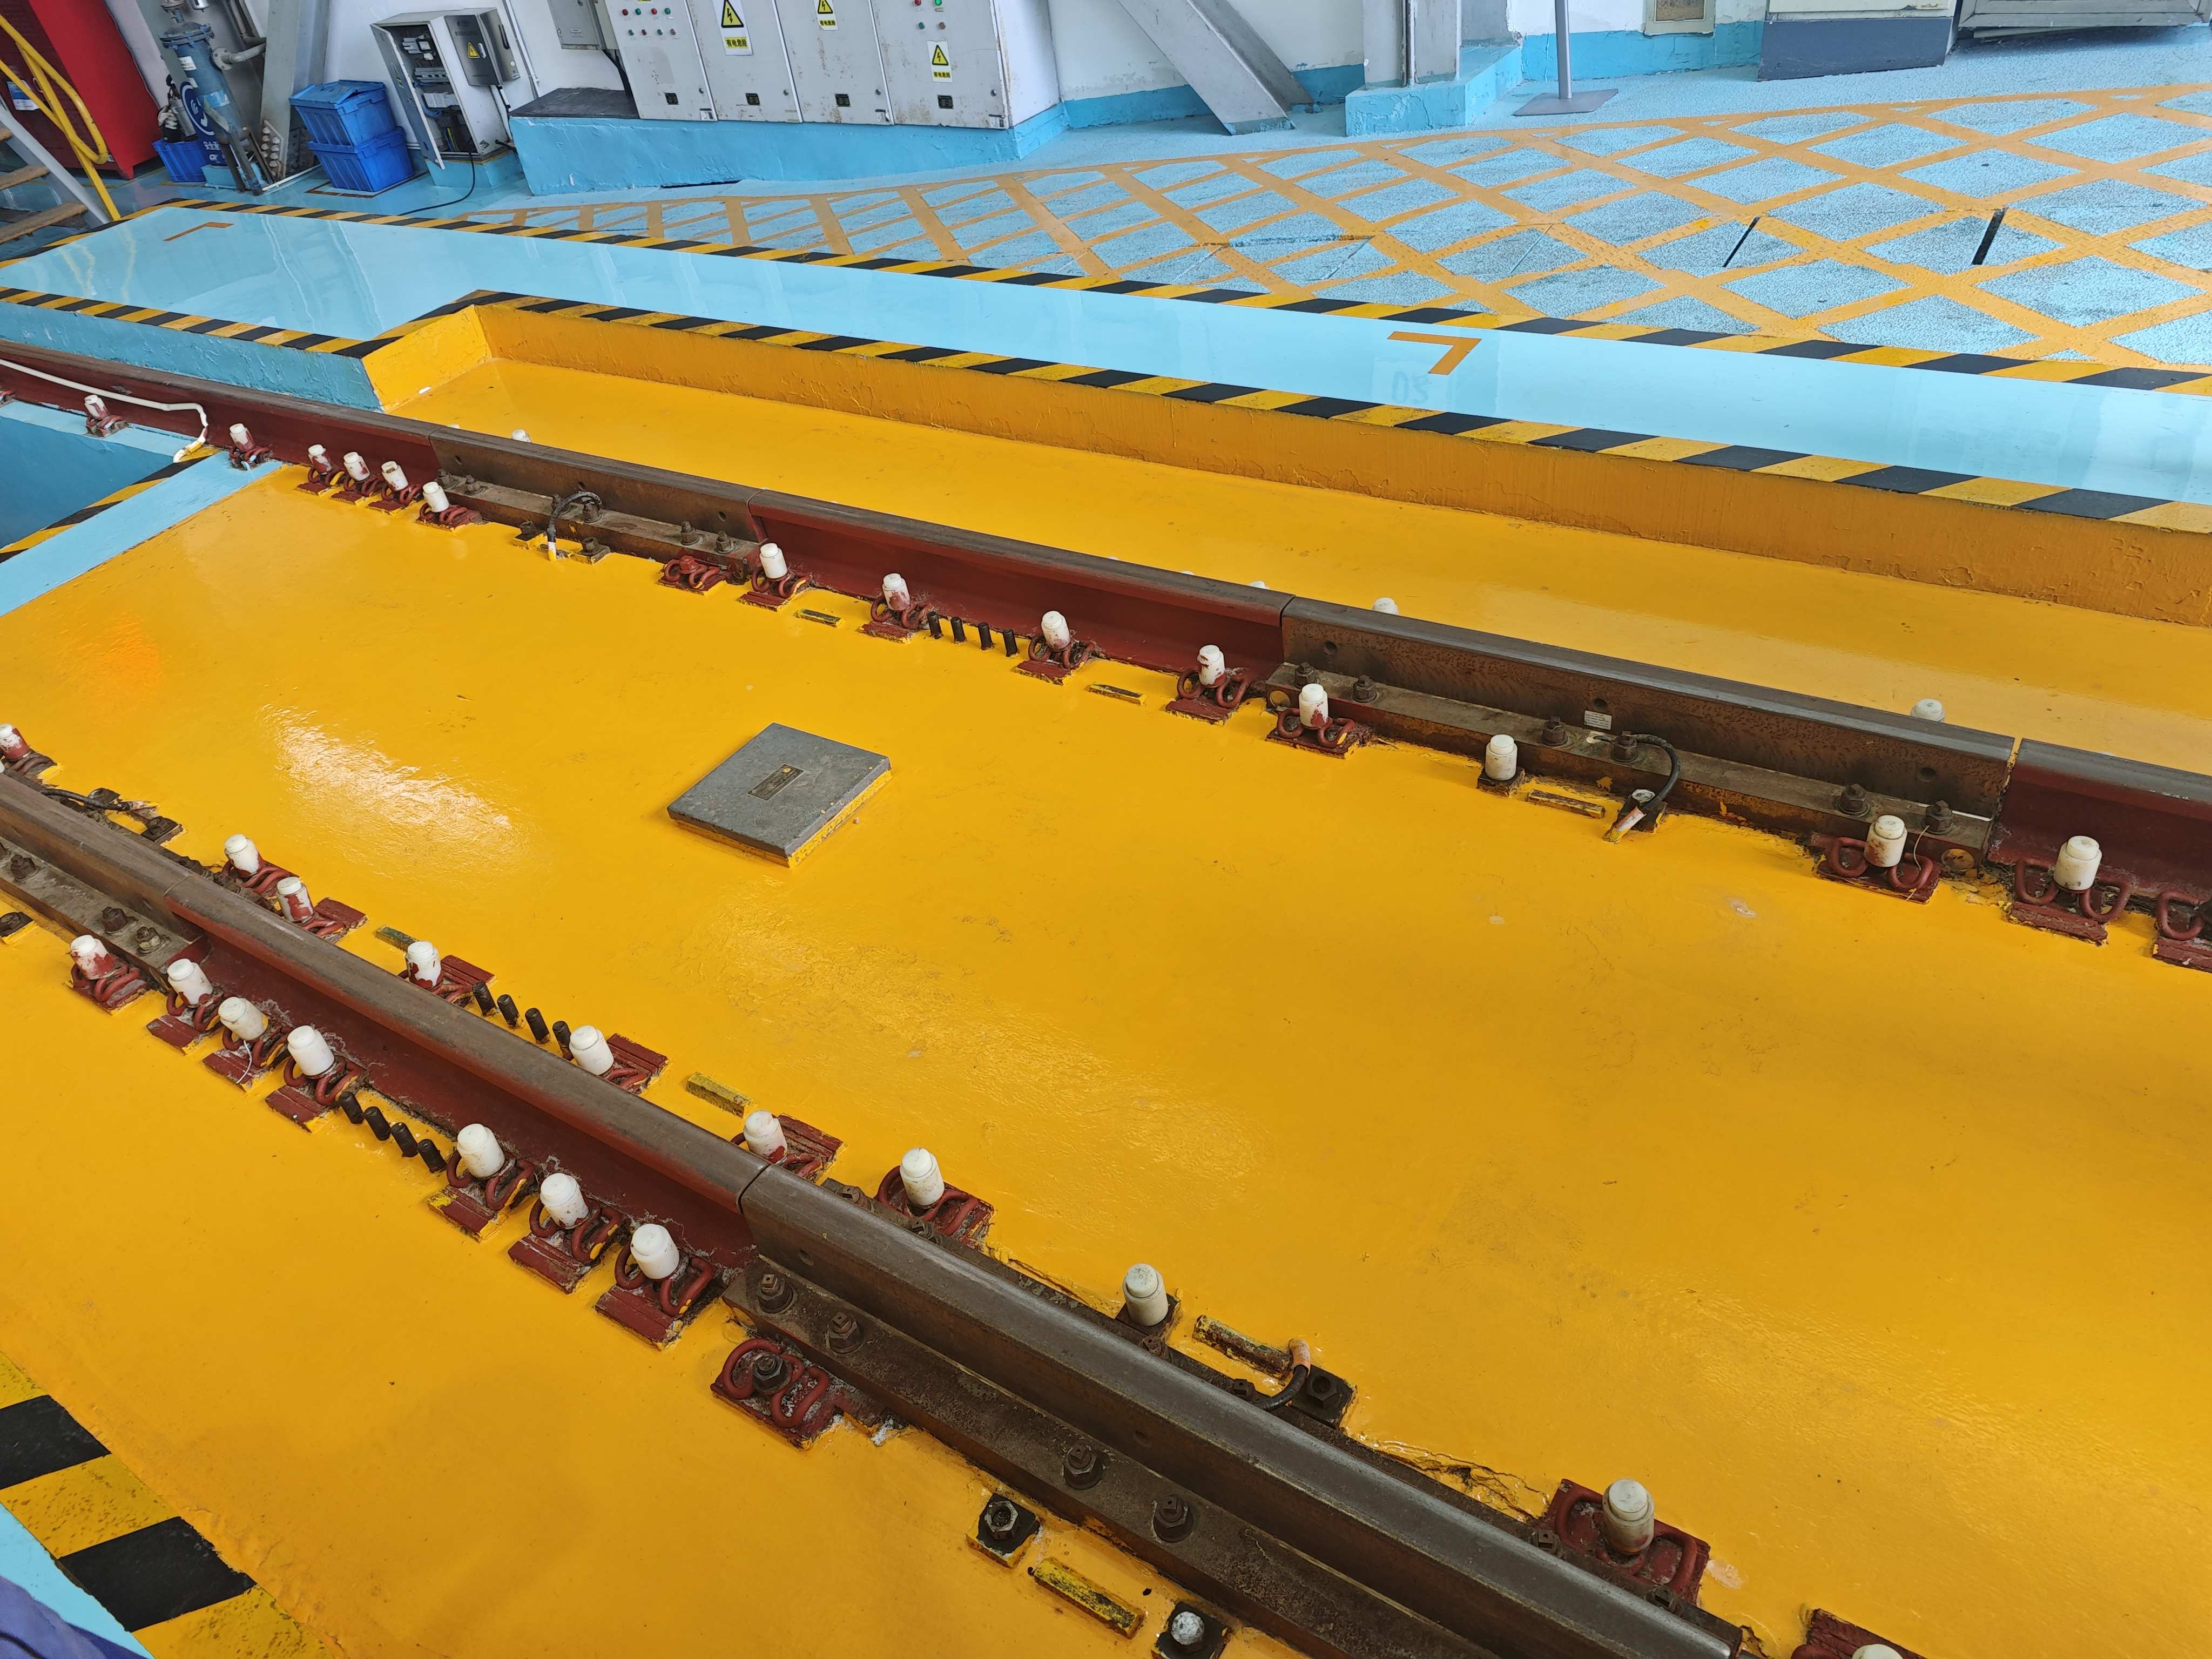
\includegraphics[width=0.32\textwidth]{assets/20260718_215423.jpg}
  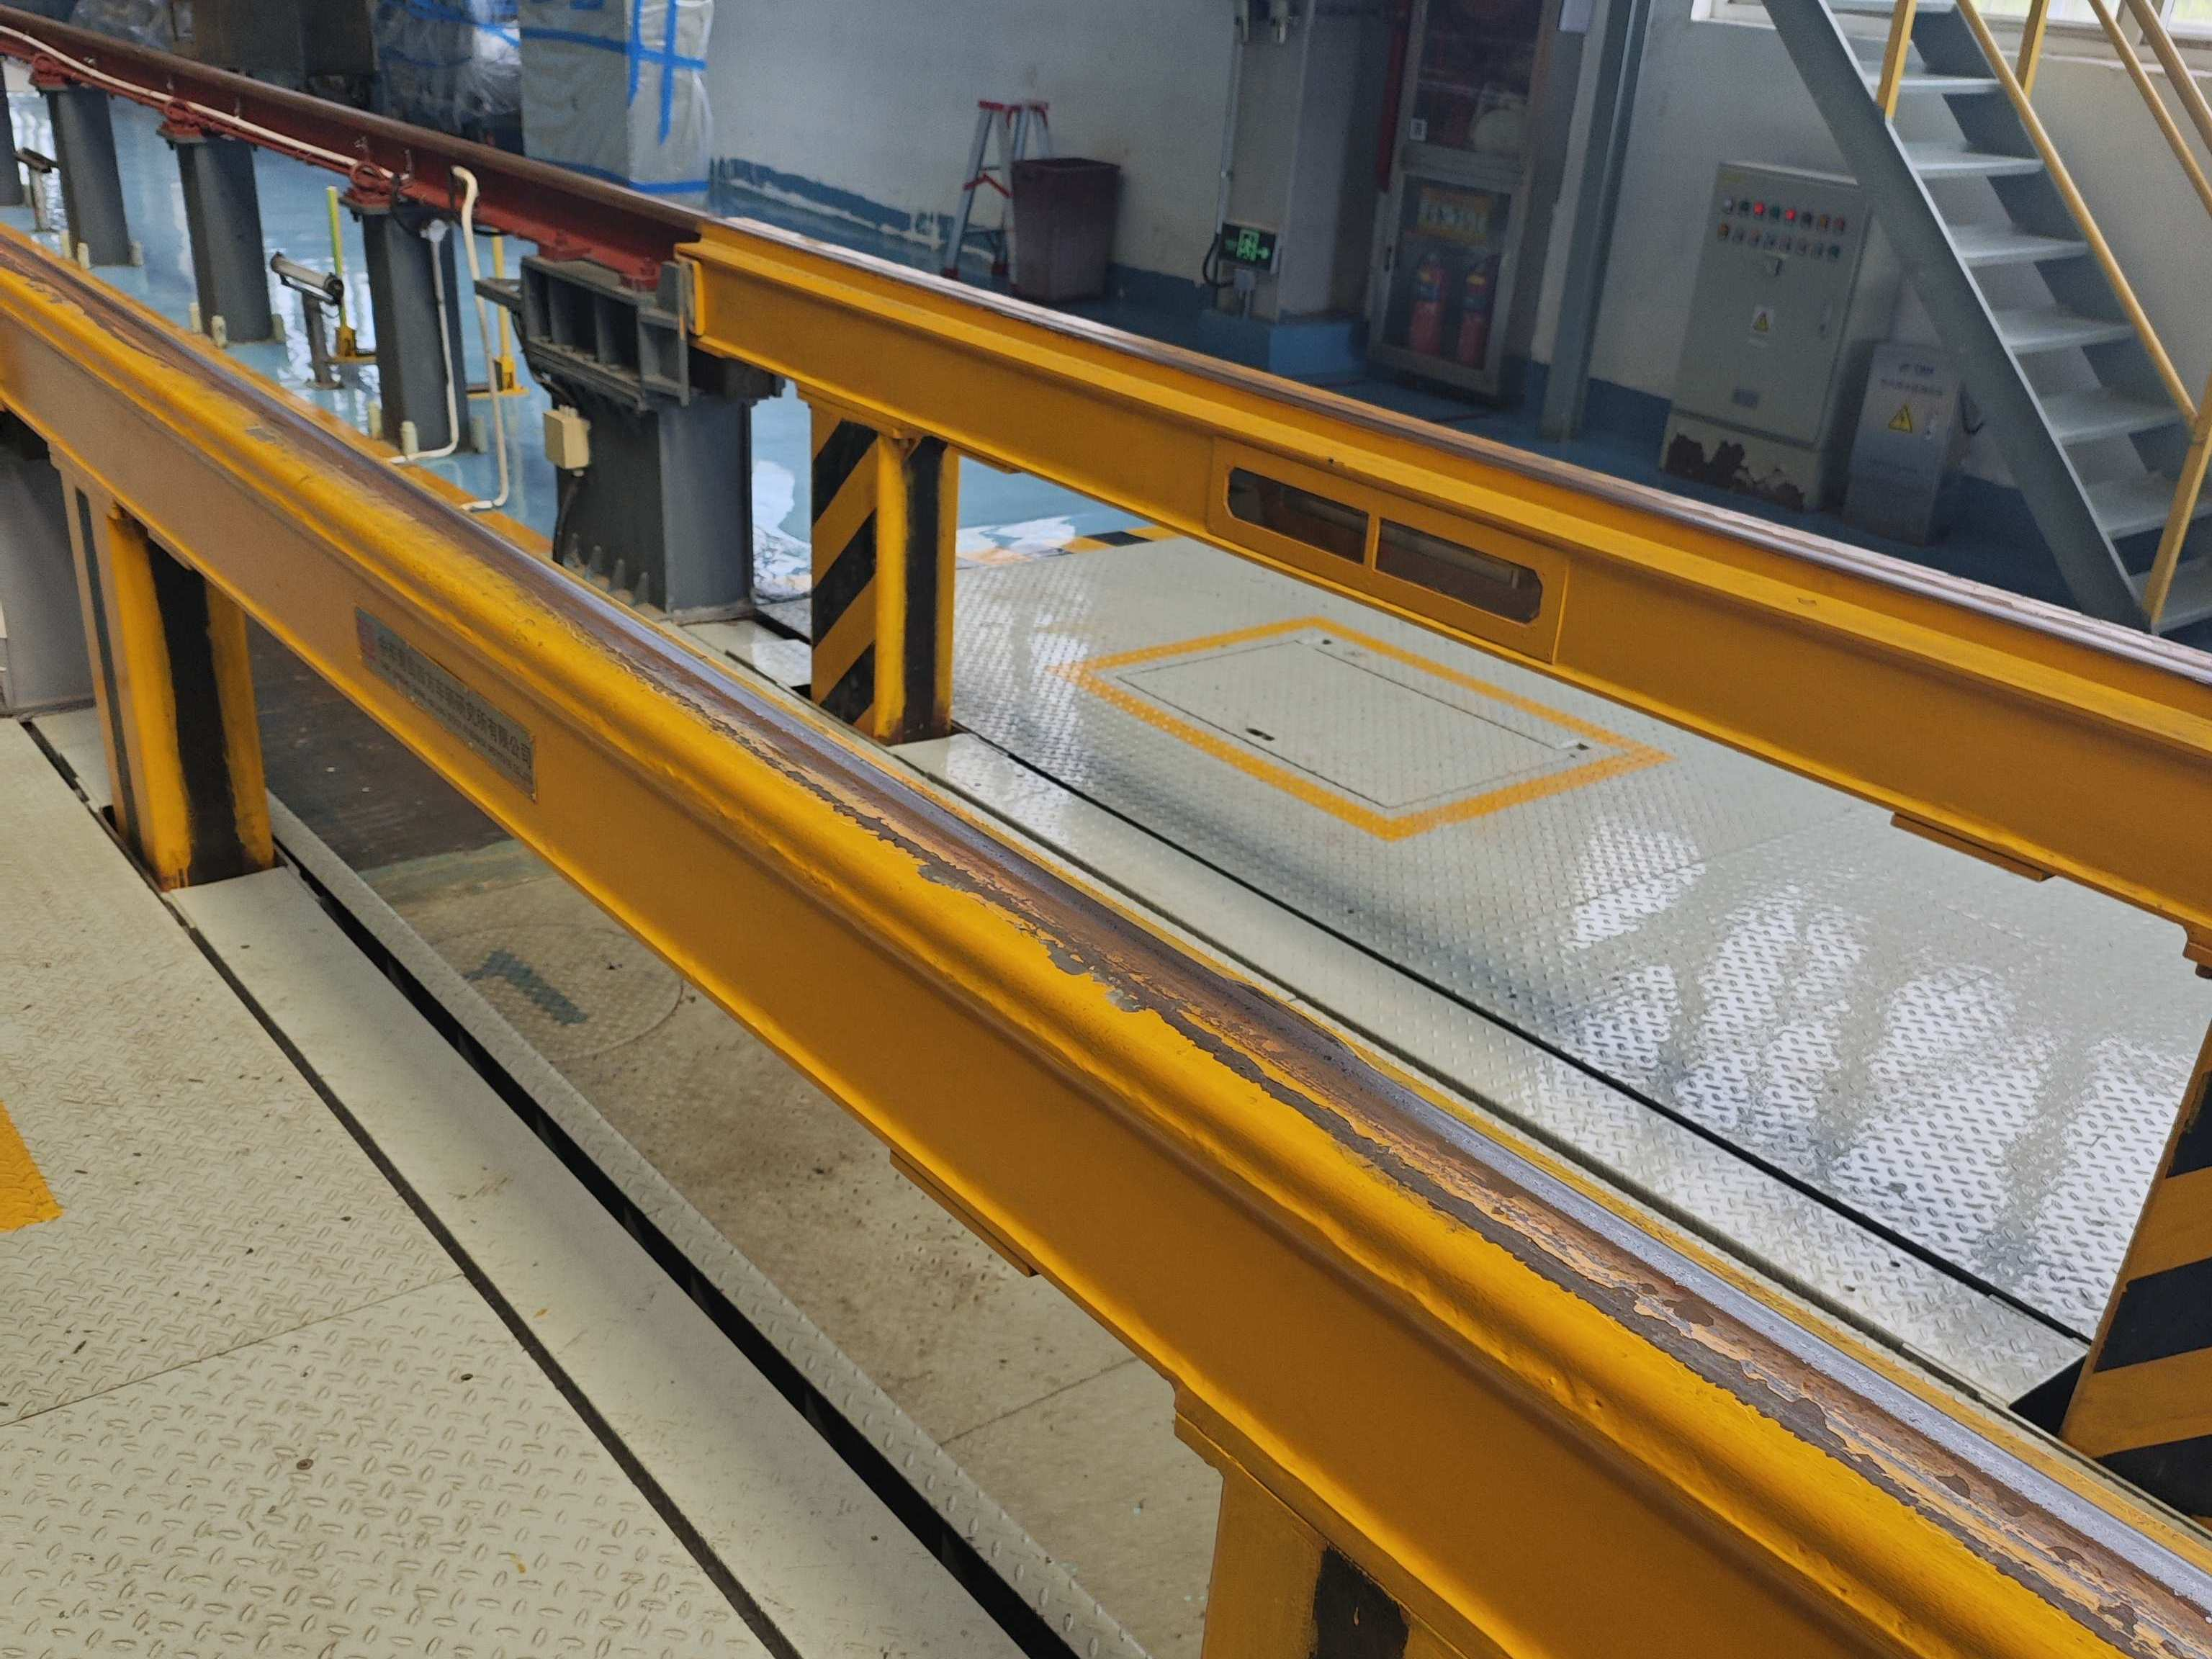
\includegraphics[width=0.32\textwidth]{assets/20260718_215429.jpg}
  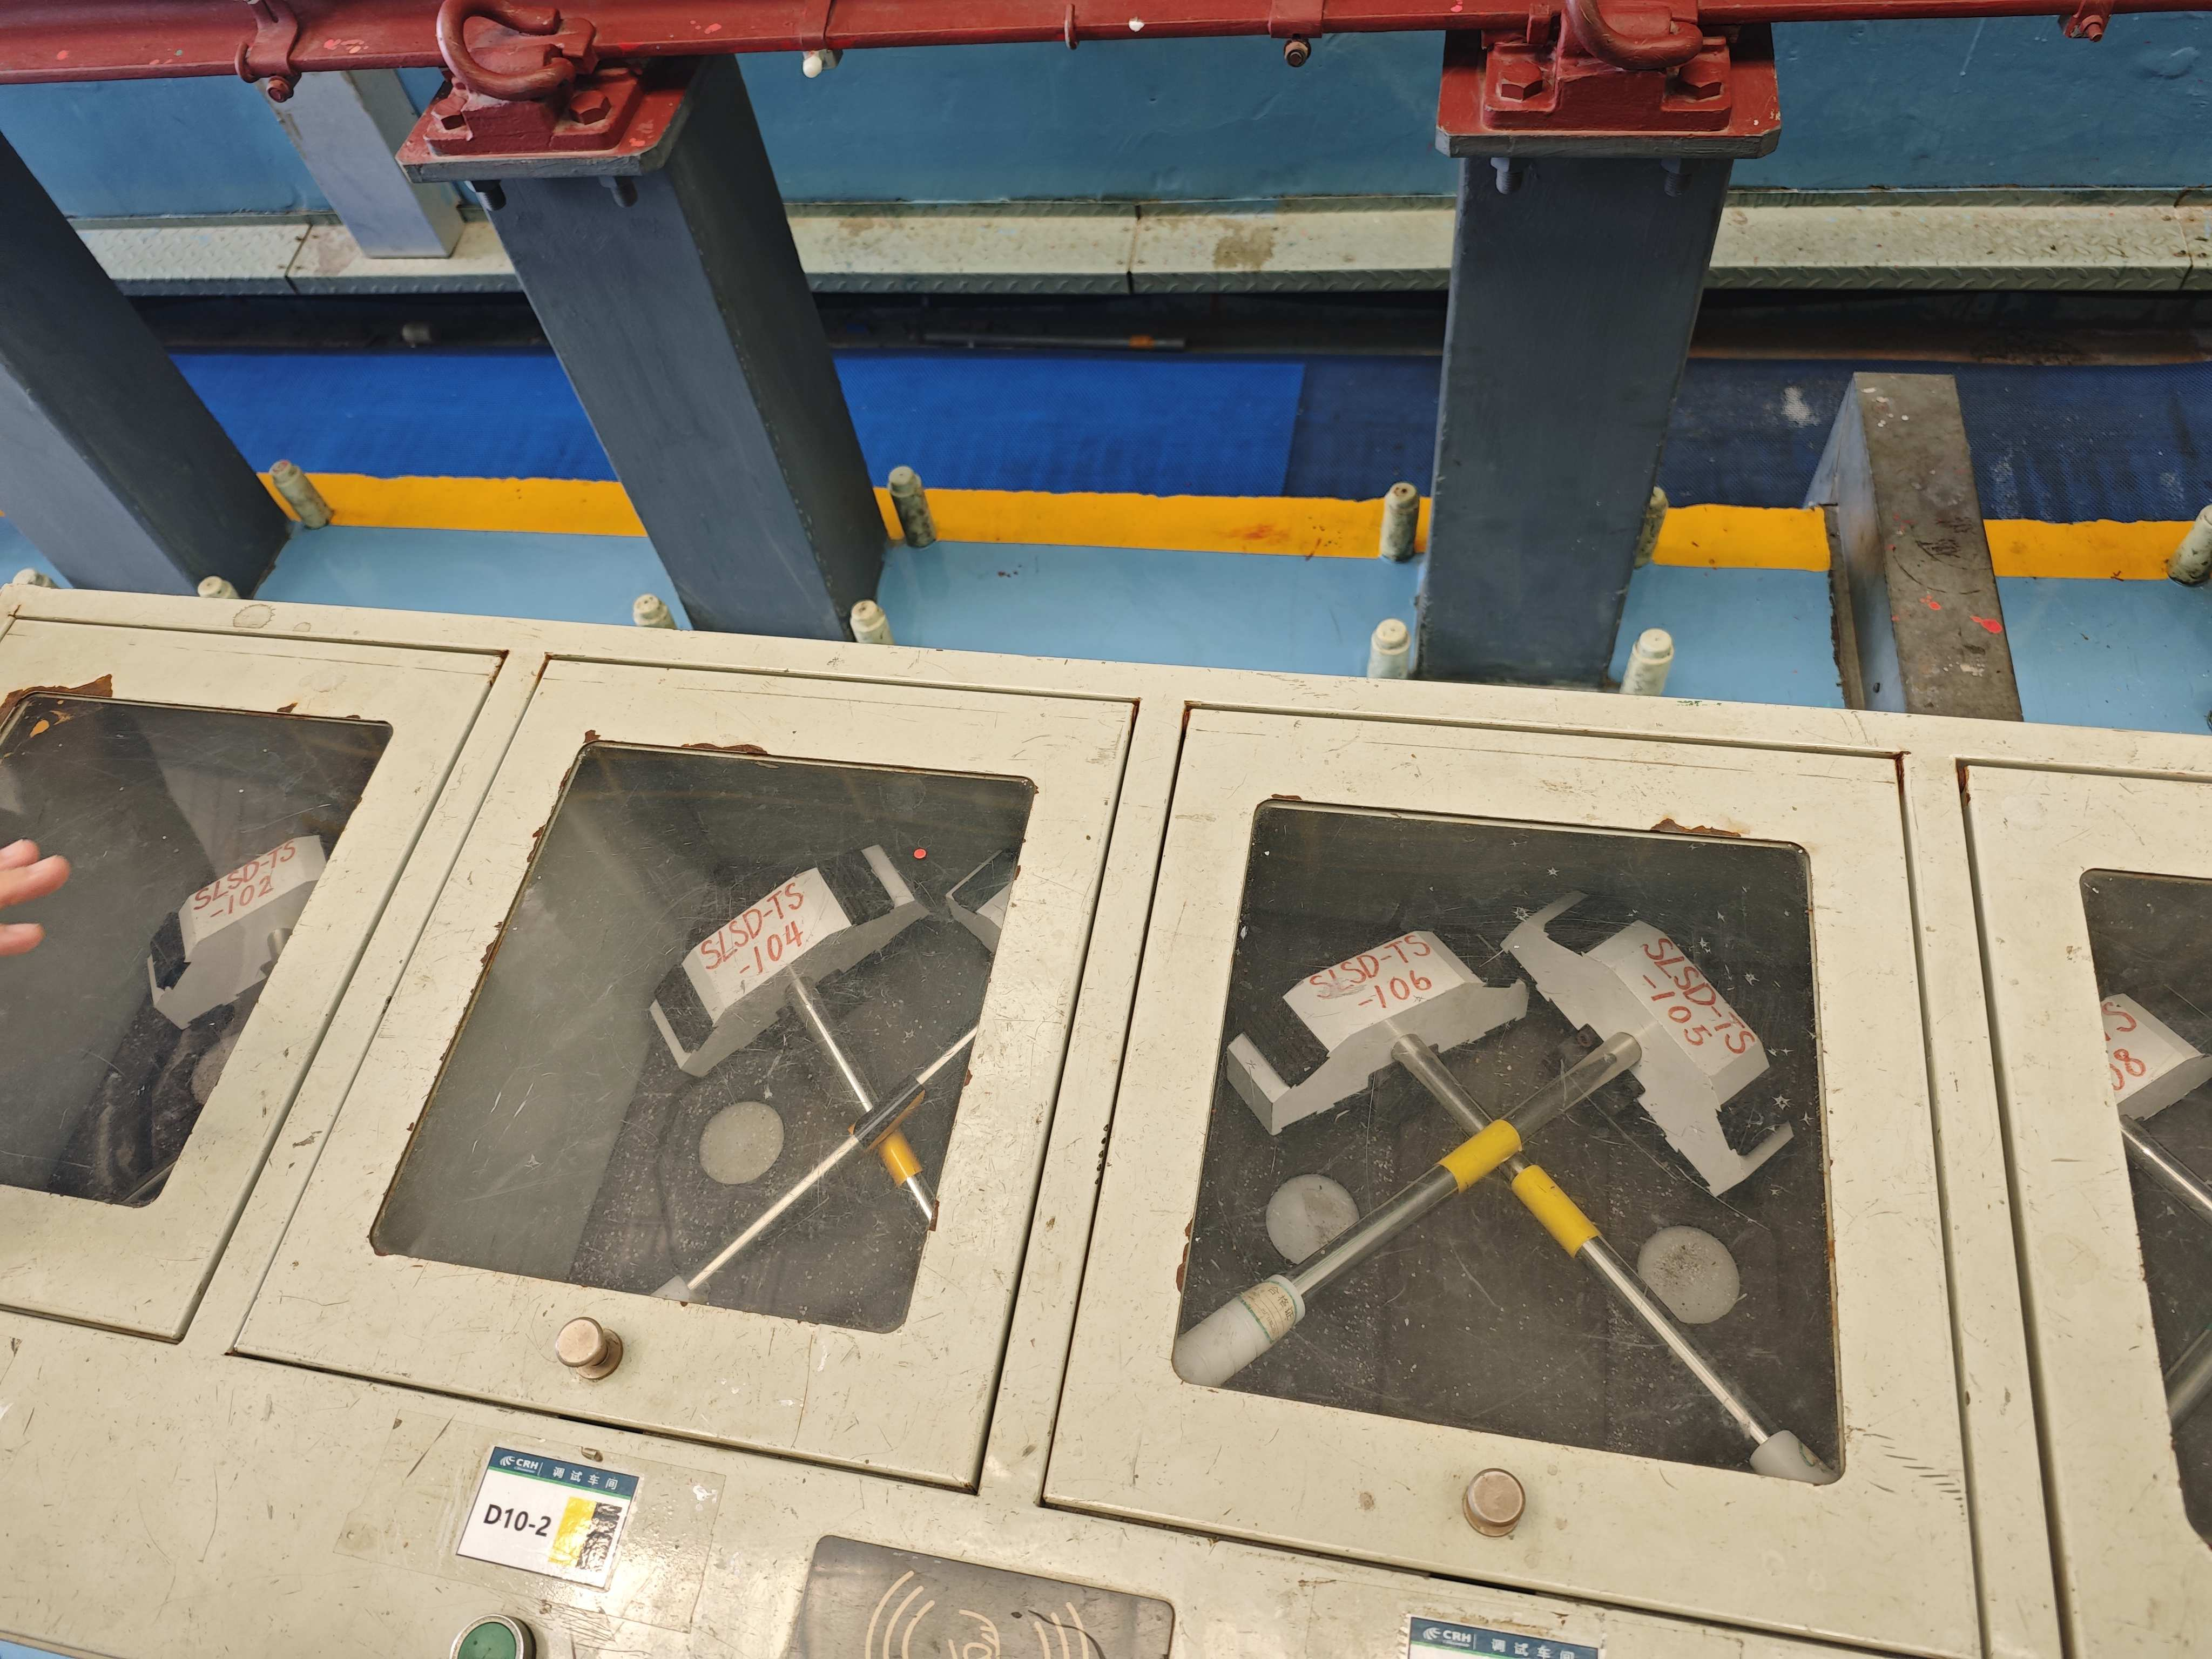
\includegraphics[width=0.32\textwidth]{assets/20260718_215456.jpg}
  \vspace{-2.5mm}
  \caption*{\small{}图22\quad{}部分检修用设备}
  \vspace{-5mm}
\end{figure}
此外，由于天气较热，工人们都是两人一组，一是有些操作一个人做不了，二是可以相互照应，防止发生中暑后无法及时发现。\par{}
\vspace{-5mm}\subsection*{二、 MCC - 高级修检修控制中心}\vspace{-2mm}
接下来我们来到了MCC，指挥中心的工作人员主要展示的是控制中心专用的数字化控制平台，上面集成了生产指挥、指标管控、数字档案、车间监控等，大量运用数字孪生技术，可以通过摄像头实时监视厂房内部的情况；工作人员展示了当前正在修理的列车的数字档案，刚刚我们参观的厂房中的CRH380BL-3545赫然在列，有详细的各项指标（前文的部分数据也是来源于此）。\par{}
令我印象最深的就是2026一季度短编（应指8节编组）三级修全路修时排\par{}

\newpage
\journalpage\par\noindent
名。修时就是指从车辆进入厂房到修竣出厂的全过程时长，其中第一名是广州局的12.4天，第二名是上海局的12.7天，第三名是成都局的13.4天……之前参观一号库的时候带队的工人师傅就说现在全路都在卷修时，从之前的近一个月变成现在的两周之内，发展非常的迅速。\par{}
\vspace{-5mm}\subsection*{三、 三号库 - 部件检修库}\vspace{-2mm}
最后我们来到了三号库，首先映入眼帘的是一个小展览区，其中有五个车上设备拆下来做的艺术品，分别体现了部件检修部门的工作理念——PARTS，即精准/Precision-能力/Ability-变革/Revolution-持续/Timeless-安全/Security。图23的小机器人的主体就是逆变器散热器（总之某种散热器）的风机电机。\par{}
\begin{figure}[H]
  \centering
  \vspace{-2.5mm}
  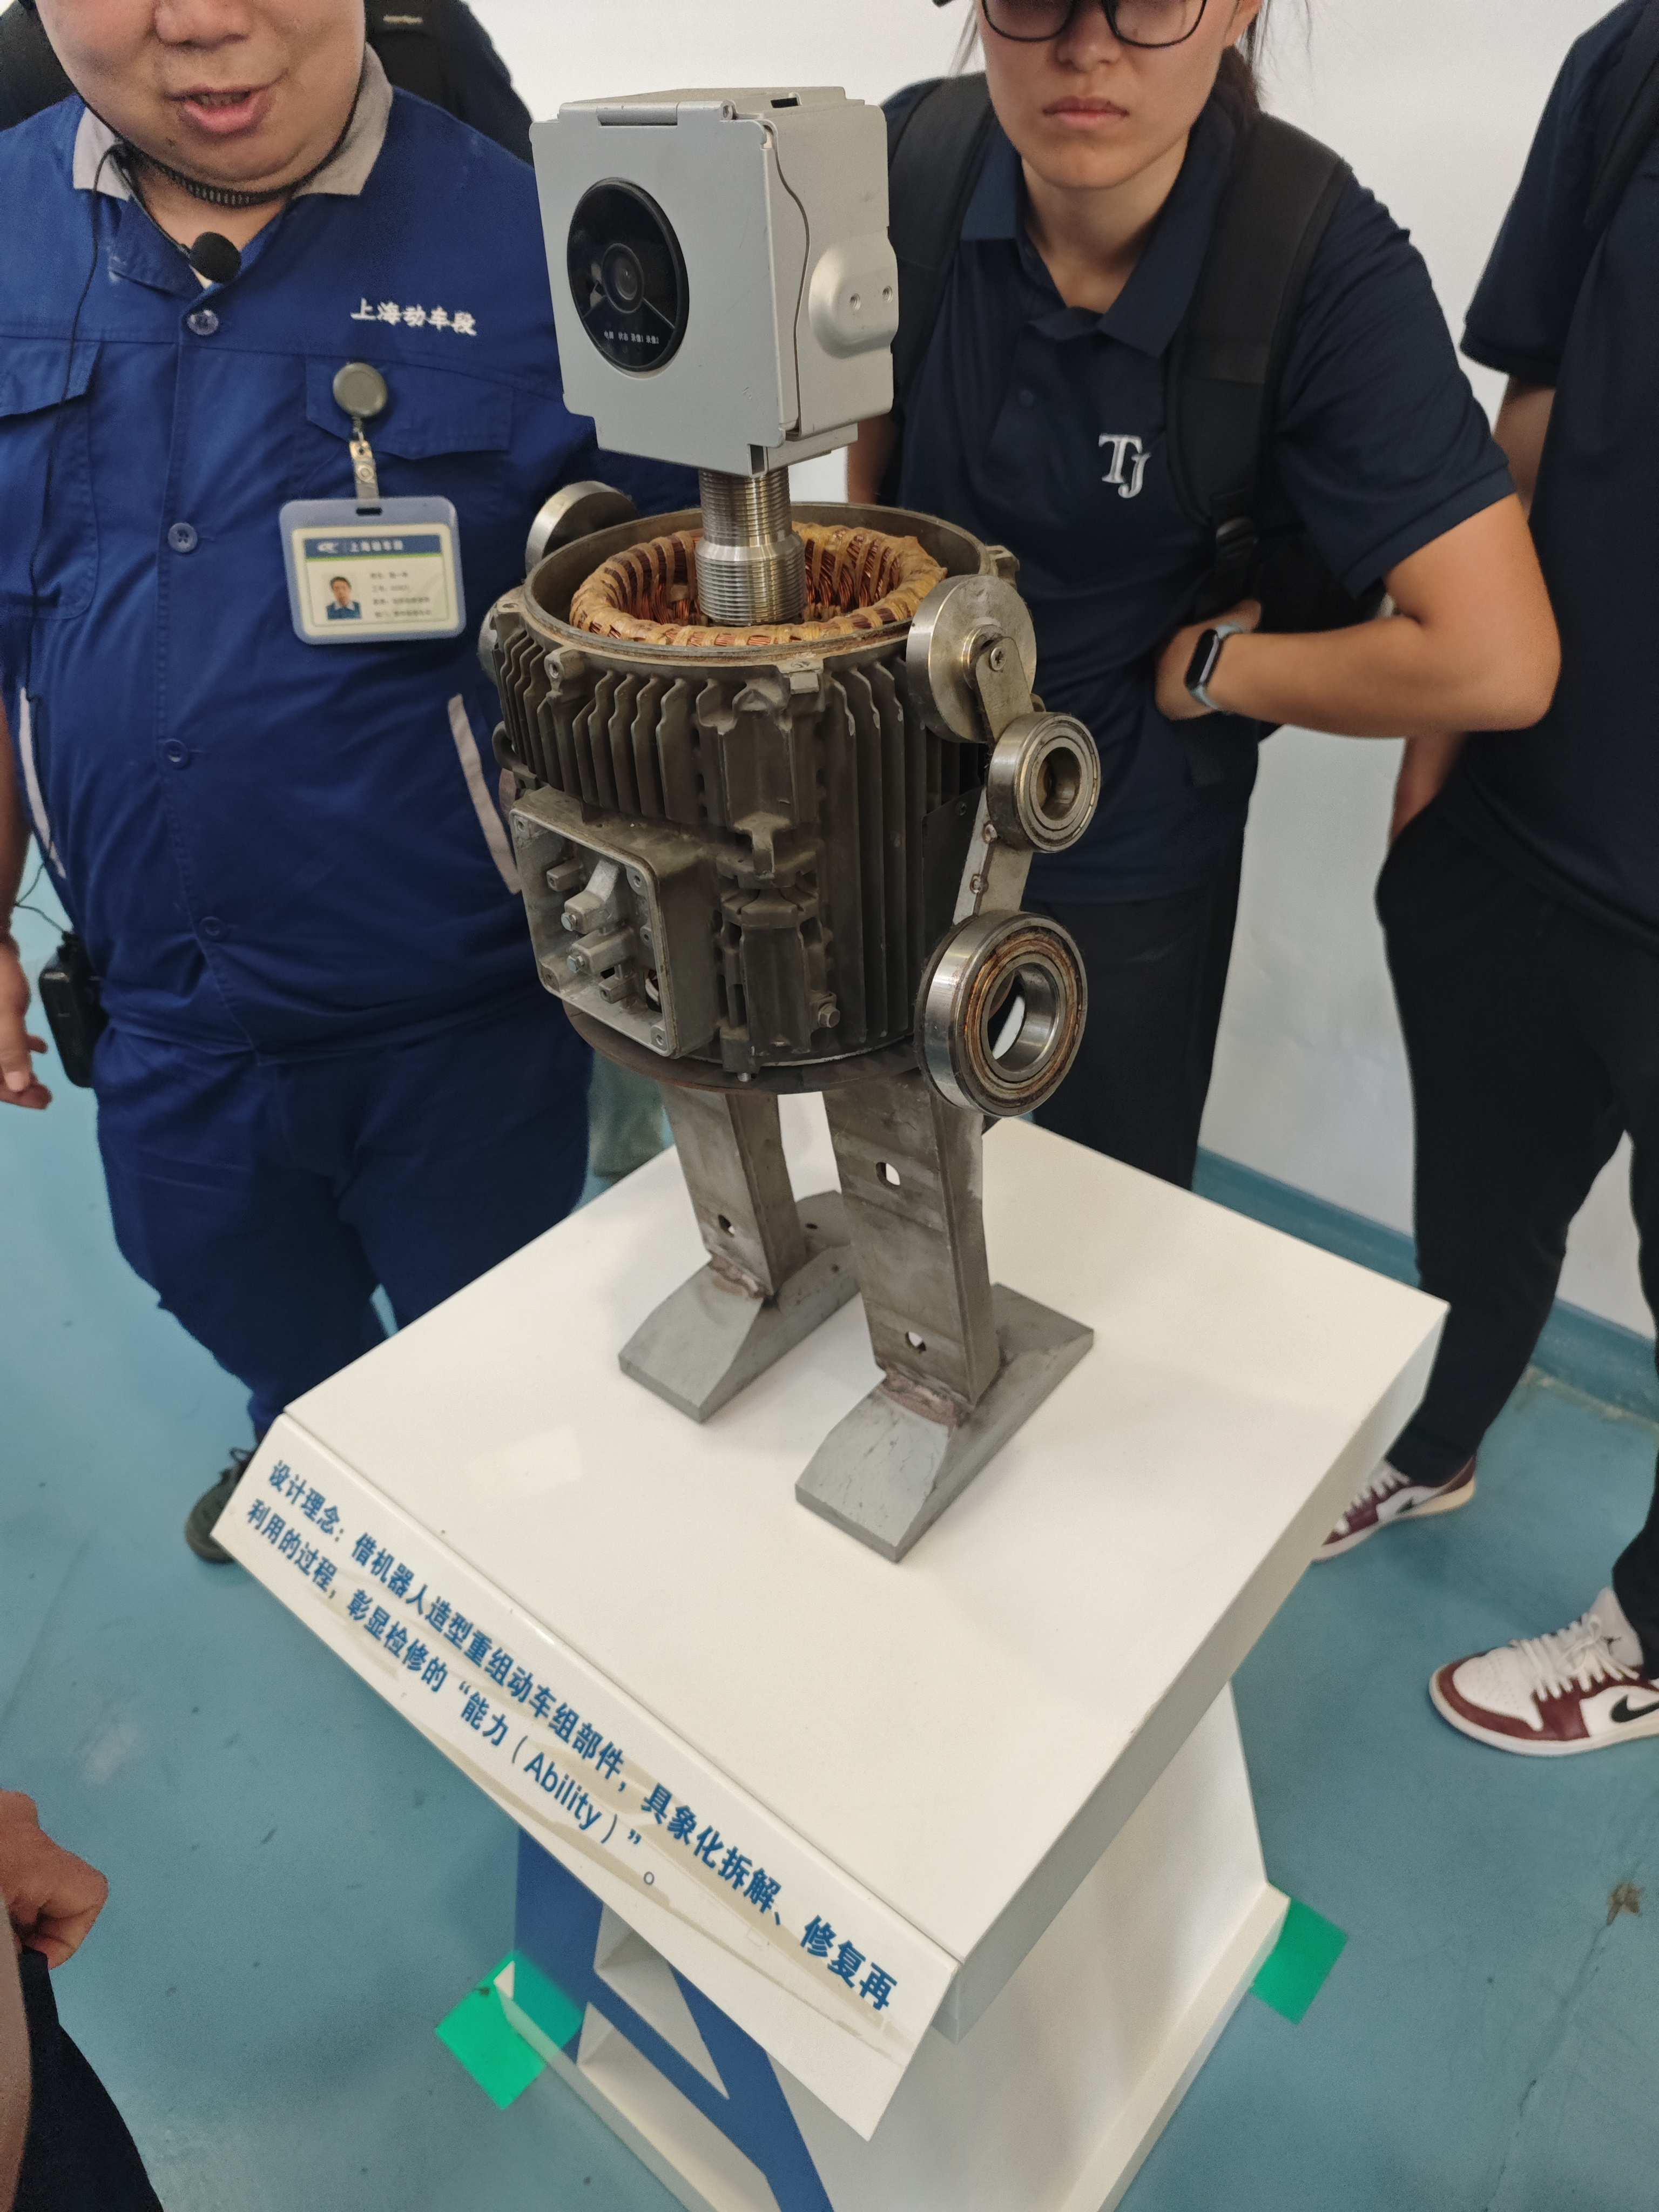
\includegraphics[width=0.6\textwidth]{assets/20260718_233942.jpg}
  \vspace{-2.5mm}
  \caption*{\small{}图23\quad{}机器人艺术品}
  \vspace{-5mm}
\end{figure}
我们参观的厂房中主要有两条产线，分别是空调检测和车钩检测产线。拆解下来的空调要经过检修、组装、试验（气密试验、淋雨试验、运转试验、焓差试验等）、交检交验、合格品存放等步骤，而车钩（主要是动车组端部的重联用车钩）则要经过零部件检查、部件探伤、预装、总装、试验、交检交验、合格品存放等步骤。\par{}
下图则展现了部分工序的工位情况，从左往右依次为：空调检修、空调组装、车钩连挂试验。\par{}

\newpage
\journalpage\par\noindent
\begin{figure}[H]
  \centering
  \vspace{-2.5mm}
  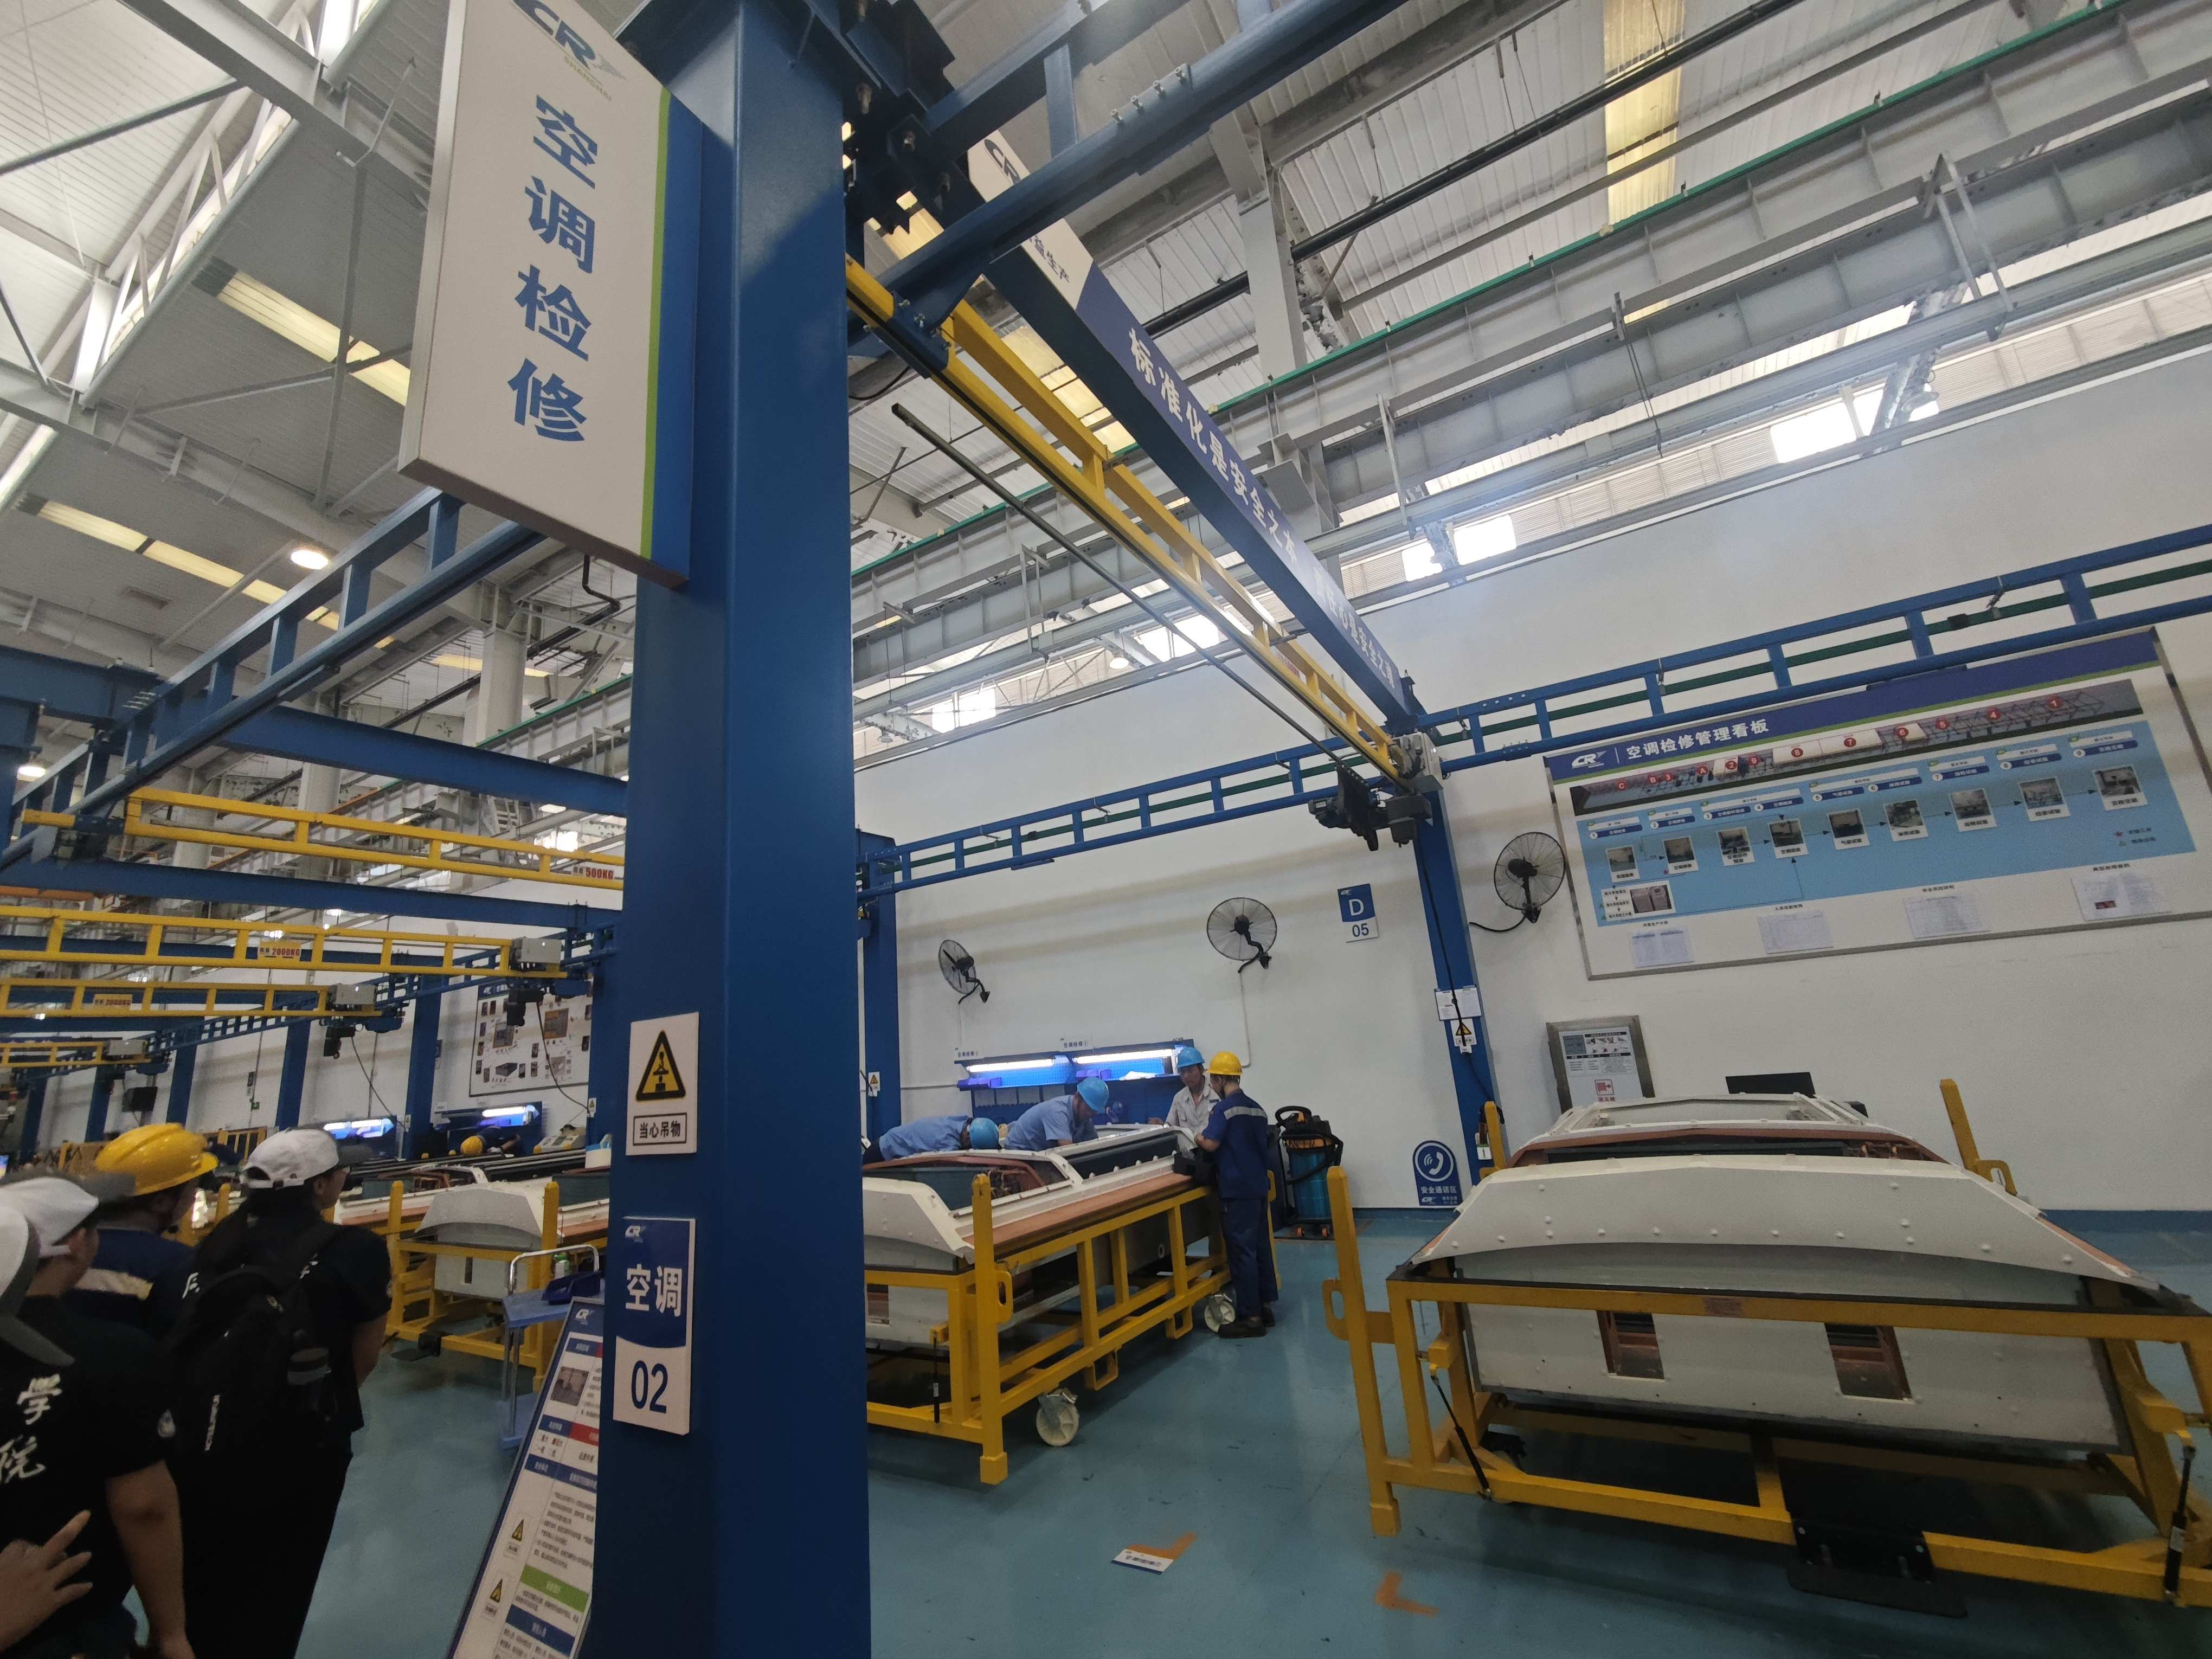
\includegraphics[width=0.32\textwidth]{assets/20260718_234723.jpg}
  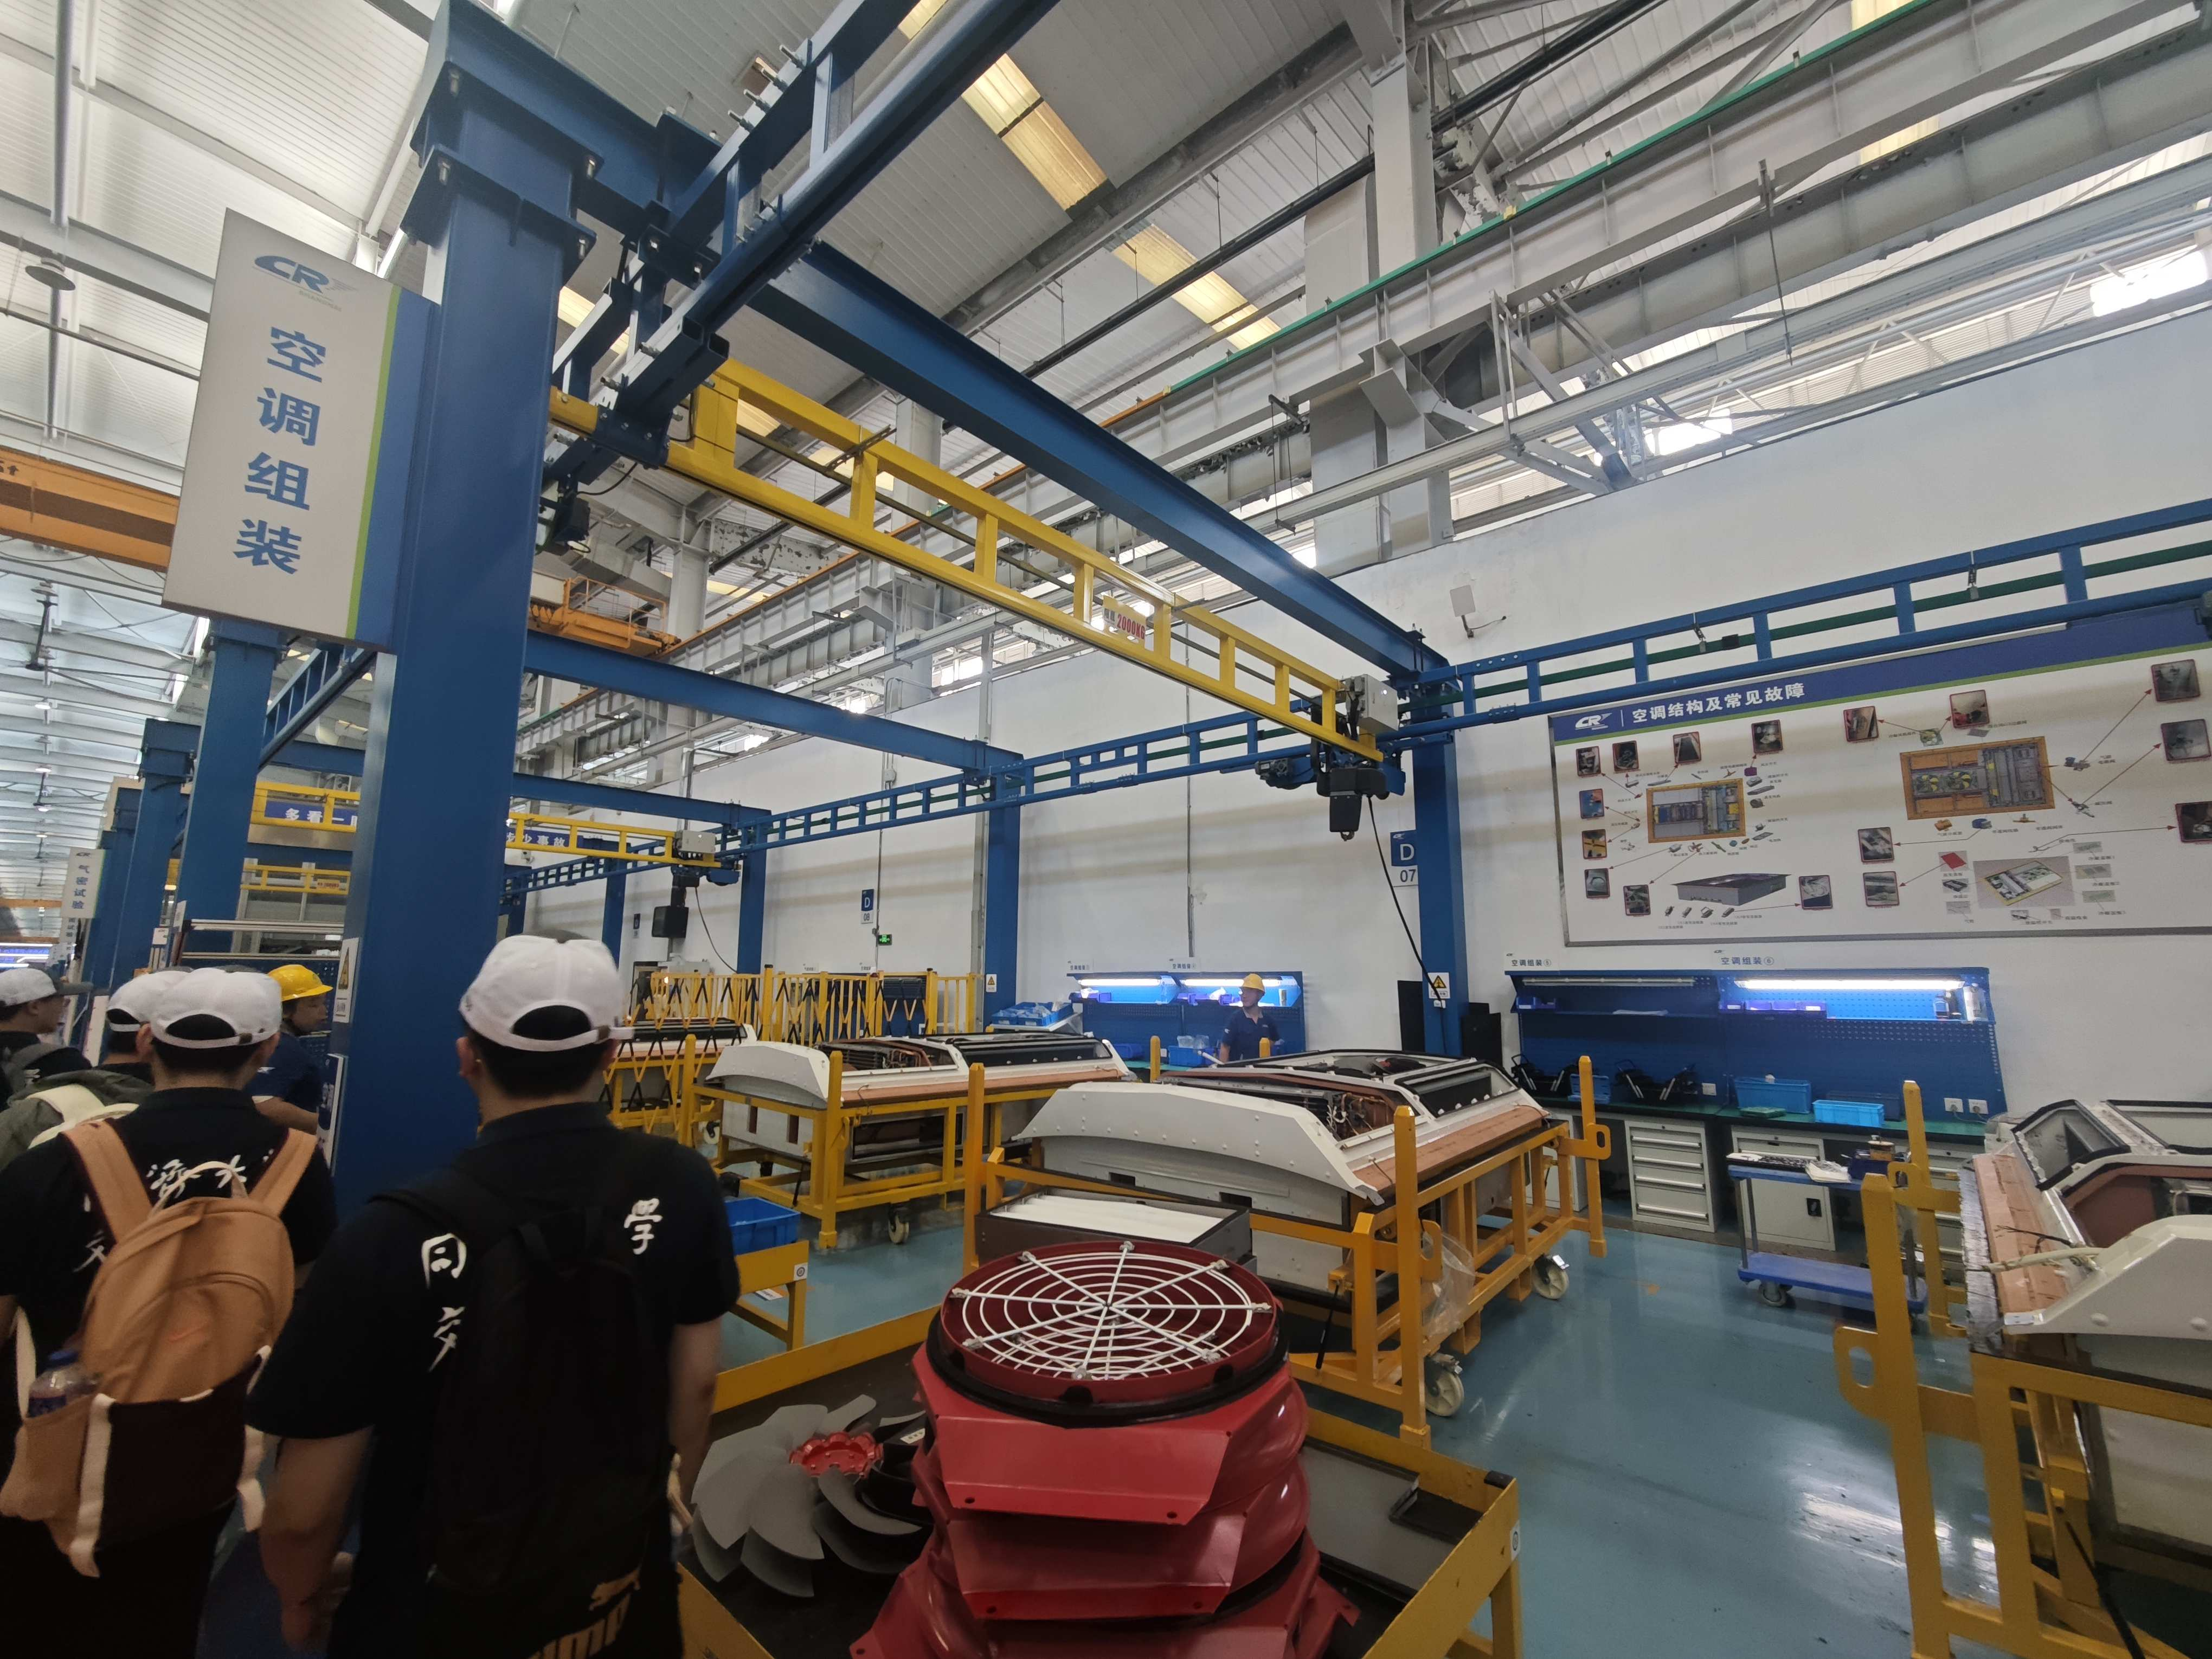
\includegraphics[width=0.32\textwidth]{assets/20260718_234735.jpg}
  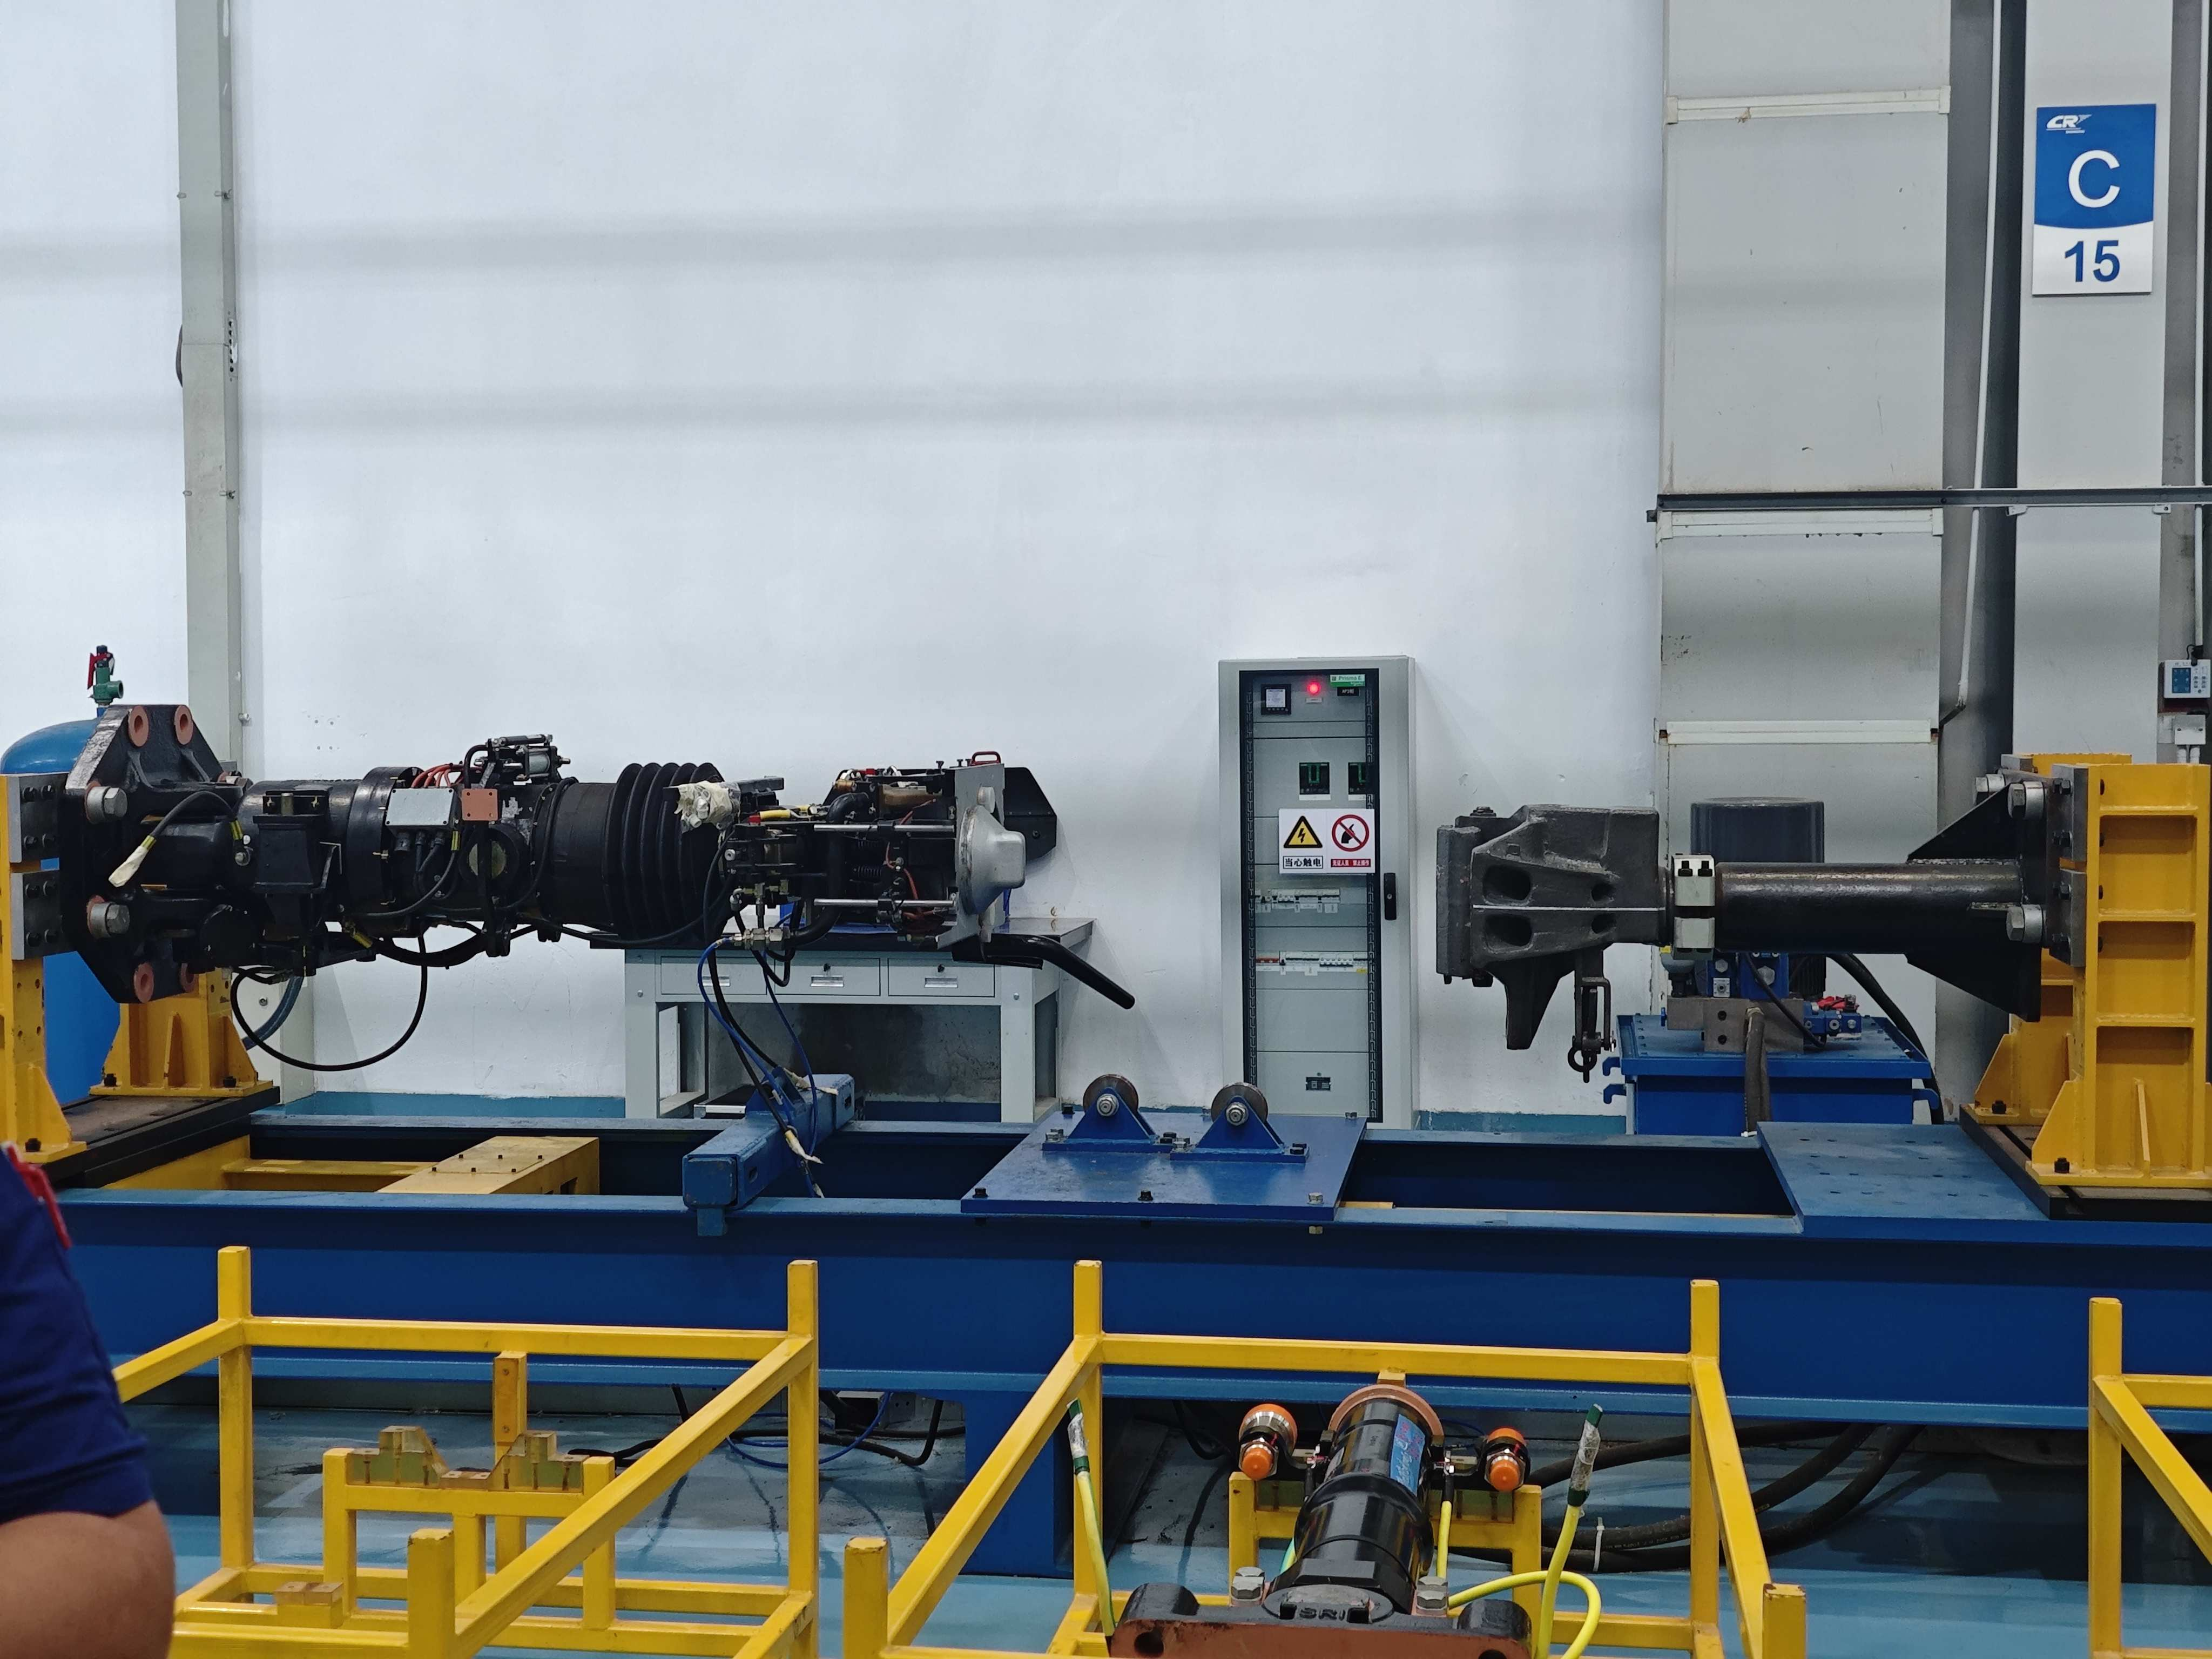
\includegraphics[width=0.32\textwidth]{assets/20260718_234802.jpg}
  \vspace{-2.5mm}
  \caption*{\small{}图24\quad{}部分工位现状}
  \vspace{-5mm}
\end{figure}
参观完这个厂房后，我们就驱车回到了学校。\par{}
总的来说，这9天的学习让我收获颇丰，学到了很多车辆制造、检修的知识，也复习了课堂知识，让这些知识不再浮空、真正落到实处；同时我们还了解了很多轨道车辆相关企业的人才培养、薪资制度等，也为后续就业打下了一定基础。希望明年的学弟学妹们也能收获满满。\par{}
\hypertarget{references}{}
\begin{flushleft}
  \begin{small}
    \ctexset{section = {format = {\raggedright\diaryHei\bfseries\Large}}}
    \begin{thebibliography}{99}
      \vspace{-3mm}
      \bibitem{ref1} 中车南京浦镇车辆有限公司. 点亮未来 圆梦智造｜带你走近科技感爆棚的焊接智能化产线 [EB/OL]. 2023-03-06 [2026-07-10].
      \href{https://crrcgc.cc/pz/2023-03/06/article\_A0C04F7DB9A24A3B8AC0887602A92DC1.html}{\color{blue} https://crrcgc.cc/pz/2023-03/06/article\_A0C04F7DB9A24A3B8AC0887602A92DC1.html}.
      \vspace{-3mm}
      \bibitem{ref2} 贵道蕉通. 【配线图】上海轨道交通全网配线V2025.26.1发布 [EB/OL]. 2026-02-23 [2026-07-13].
      \href{https://mp.weixin.qq.com/s/sL8Ps5r06D0HnVSF5U9x5w}{\color{blue} https://mp.weixin.qq.com/s/sL8Ps5r06D0HnVSF5U9x5w}.
      \vspace{-3mm}
      \bibitem{ref3} 中国铁路总公司. 和谐3C/380B{(L)}/380BG/380CL型动车组三级检修规程: TG/CL151-2017 [S/OL]. 北京: 中国铁路总公司, 2017[2026-07-18].
      \href{https://www.nra.gov.cn/jglz/fgzd/gfwj/201803/P020220801567210163768.pdf}{\color{blue} https://www.nra.gov.cn/jglz/fgzd/gfwj/201803/P020220801567210163768.pdf}.
    \end{thebibliography}
    \ctexset{section = {format = {\centering\diaryHei\bfseries\Large}}}
  \end{small}
\end{flushleft}

\end{document}
